\documentclass{WitsPhysicsReport}
%------------------------------------------------------------
% Using WitsPhysicsReportUtil style
\usepackage{WitsPhysicsReportUtil}
%------------------------------------------------------------
% Set Details
% \Title{Solving Partial Differential Equations Using Reservoir Computing: An Application To Iterative Image Segmentation}
\Title{Learning Level Set Method by Echo State Network for Image Segmentation}

\begin{document}

\maketitle

\section{Introduction}
\label{sec:Introduction}

\subsection{Problem statement and motivation}
\label{sec: Introduction_to_sequence_model}




Modeling of temporal (i.e time dependency) tasks form a vital part within many fields of research (e.g speech recognition, character recognition, dynamical system). The problem of modeling temporal tasks is referred as \textit{time series prediction} (i.e to estimate of future events of the time series based on previously observed events). Such estimates may be obtained from a mathematical model of the mechanisms which generate the time series. If there are known fundamental deterministic equations, they can be used to predict future observations based on the knowledge of initial conditions. 

In practice, it is very often the case that insufficient or no physical knowledge about the mechanisms generating the time series is available, rendering the deductive approach to modeling impossible. In this case the "rules" that these mechanisms must be inferred from regularities in past observations. These rules may be specified as an assumed functional relationship between the previous and future events of the time series.

Over the past decade, a successful implementation of these functional relationships which provide a mapping from previous observation onto estimates of future events, is \textit{artificial-neural-networks} (ANNs), particularly \text{feed-forward networks (FNNs)} as shown in Figure~\ref{fig:Recurrent_Neural_Network_(RNN).} (right). These networks have proven to be reliable tools in many problems. FNNs are stateless (i.e. having no memory) networks, although the were some successful application to time series problems, due to the lack of memory they struggle to infer current events based on previous events. This was later solved through the introduction of feedback connections (i.e. loops) from the output of the units back to their inputs in the connectivity of the FNNs, referred to as \textit{recurrent-neural network (RNNs)}. The advantage of RNNs compared to FNNs is their ability to model temporal events (i.e. time depend events) is due to the internal \text{memory} introduced by the feedback connections as shown in Figure~\ref{fig:Recurrent_Neural_Network_(RNN).} (left).



\begin{figure}[H]
\centering
\tikzstyle{pla}=[circle,draw,draw=black!50,fill=blue!10,inner sep=0pt,minimum size=2mm]
\tikzstyle{do}=[circle,draw=black!50,fill=black!30,inner sep=0.2pt]
\begin{tikzpicture}[node distance = 1.5cm, thick, nodes = {align = center},>=latex]
% Input nodes
\node[pla] (A) {};
\node[pla] (B) [below of=A]  {};
\node[pla] (C) [below of=B]  {};
\node[do] (D) [below of=C] {};
\node[pla] (E) [below of=D]  {};
%\node (inn)[above of=A] {\color{red} Input layer}; 
\node[rectangle, draw=black,draw=red!60, fit=(A) (B) (C) (D) (E) , inner sep=1mm] (all) {};
% Hidden nodes
\node[pla] (h1) [right of= A]  {};
\node[pla] (h2) [below of=h1]  {};
\node[pla] (h3) [below of=h2]  {};
\node[do] (h4) [below of=h3] {};
\node[pla] (h5) [below of=h4]  {};
\node[pla] (h6) [right of= h1]  {};
\node[pla] (h7) [below of=h6]  {};
\node[pla] (h8) [below of=h7]  {};
\node[do] (h9) [below of=h8] {};
\node[pla] (h10) [below of=h9]  {};
%\node (in)[right=1.0cm of inn] {\color{blue} Hidden Layer}; 
\node[rectangle, draw=black, fit=(h1) (h2) (h3) (h4) (h5) (h6) (h7) (h8) (h9) (h10), inner sep=1mm, draw=blue!60] (hidden) {};
%Output node
\node[pla] (o1)  [right of = h8] {};
%\node (inh) [right=0.0cm and 2.5cm of inn] {\color{green} Output Layer}; 
% \node (inr) [font=\fontsize{10}{0}\selectfont, below =1.5cm of h9] { \color{red} Recurrent connection}; 
\node[rectangle, draw=black,draw=green!60, fit=(o1) (o1), inner sep=1mm] (out) {};
% Input--Hidden arrows
\draw [black,thick,->] (A) to (h1);
\draw [black,thick,->] (A) to (h2);
\draw [black,thick,->] (A) to (h3);
\draw [black,dotted,->] (A) to (h5);
\draw [black,thick,->] (B) to (h1);
\draw [black,thick,->] (B) to (h2);
\draw [black,thick,->] (B) to (h3);
\draw [black,dotted,->] (B) to (h5);
\draw [black,thick,->] (C) to (h1);
\draw [black,thick,->] (C) to (h2);
\draw [black,thick,->] (C) to (h3);
\draw [black,dotted,->] (C) to (h5);
\draw [black,dotted,->] (E) to (h1);
\draw [black,dotted,->] (E) to (h2);
\draw [black,dotted,->] (E) to (h3);
\draw [black,dotted,->] (E) to (h5);
\draw [black,thick,->] (h1) to (h6);
\draw [black,thick,->] (h1) to (h7);
\draw [black,thick,->] (h1) to (h8);
\draw [black,dotted,->] (h1) to (h10);
\draw [black,thick,->] (h2) to (h6);
\draw [black,thick,->] (h2) to (h7);
\draw [black,thick,->] (h2) to (h8);
\draw [black,dotted,->] (h2) to (h10);
\draw [black,thick,->] (h3) to (h6);
\draw [black,thick,->] (h3) to (h7);
\draw [black,thick,->] (h3) to (h8);
\draw [black,dotted,->] (h3) to (h10);
\draw [black,dotted,->] (h5) to (h6);
\draw [black,dotted,->] (h5) to (h7);
\draw [black,dotted,->] (h5) to (h8);
\draw [black,dotted,->] (h5) to (h10);
% Hidden--output arrows
\draw [black,thick,->] (h6) to (o1);
\draw [black,thick,->] (h7) to (o1);
\draw [black,thick,->] (h8) to (o1);
\draw [black,dotted,->] (h10) to (o1);
\tikzset{square arrow/.style={%
    -{Stealth[length=1mm]},rounded corners,draw=red,thick,%
    to path={-- ++(0,-0.5) -| (\tikztotarget)}}
                              }
\draw[square arrow]  (h10) to (h5) ;
\end{tikzpicture}
% \caption{Schematic of a recurrent neural network. The recurrent connection in the hidden layer allows information to persist from one input to another.}
% \label{fig: Recurrent_Neural_Network_(RNN)}
\hspace{6mm}
\begin{tikzpicture}[node distance = 1.5cm, thick, nodes = {align = center},>=latex]
\centering
% Input nodes
\node[pla] (A) {};
\node[pla] (B) [below of=A]  {};
\node[pla] (C) [below of=B]  {};
\node[do] (D) [below of=C] {};
\node[pla] (E) [below of=D]  {};
%\node (inn)[below of=E] {\color{red} Input layer}; 
\node[rectangle, draw=black,draw=red!60, fit=(A) (B) (C) (D) (E) , inner sep=1mm] (all) {};
% Hidden nodes
\node[pla] (h1) [right= of A]  {};
\node[pla] (h2) [below of=h1]  {};
\node[pla] (h3) [below of=h2]  {};
\node[do] (h4) [below of=h3] {};
\node[pla] (h5) [below of=h4]  {};
%\node (in)[below of=h5] {\color{blue} Hidden Layer}; 
\node[rectangle, draw=black, fit=(h1) (h2) (h3) (h4) (h5), inner sep=1mm, draw=blue!60] (hidden) {};
%Output node
\node[pla] (o1)  [right= of h3] {};
%\node (inh) [right=0.0cm and 0.5cm of in] {\color{green} Output Layer}; 
\node[rectangle, draw=black,draw=green!60, fit=(o1) (o1), inner sep=1mm] (out) {};
% Input--Hidden arrows
\draw [black,thick,->] (A) to (h1);
\draw [black,thick,->] (A) to (h2);
\draw [black,thick,->] (A) to (h3);
\draw [black,dotted,->] (A) to (h5);
\draw [black,thick,->] (B) to (h1);
\draw [black,thick,->] (B) to (h2);
\draw [black,thick,->] (B) to (h3);
\draw [black,dotted,->] (B) to (h5);
\draw [black,thick,->] (C) to (h1);
\draw [black,thick,->] (C) to (h2);
\draw [black,thick,->] (C) to (h3);
\draw [black,dotted,->] (C) to (h5);
\draw [black,dotted,->] (E) to (h1);
\draw [black,dotted,->] (E) to (h2);
\draw [black,dotted,->] (E) to (h3);
\draw [black,dotted,->] (E) to (h5);
% Hidden--output arrows
\draw [black,thick,->] (h1) to (o1);
\draw [black,thick,->] (h2) to (o1);
\draw [black,thick,->] (h3) to (o1);
\draw [black,dotted,->] (h5) to (o1);
\end{tikzpicture}
\caption{Schematic of a neural network. (left) Recurrent Neural Network (RNN). (right) Feed-forward neural network (FNN)}
\label{fig:Recurrent_Neural_Network_(RNN).}
%\label{fig: Feed-forward_Neural_Network_(FNN)}
\end{figure}



RNNs were proposed in the  80's for solving time series problems~\cite{elman1990finding,rumelhart1986learning, werbos1988generalization}. The structure of RNNs are akin to that of a multi-layer perception or feed-forward network, the fundamental difference is that the latter posses cycles (loops) in the hidden  units~\cite{lukovsevivcius2009reservoir}, as shown in Figure~\ref{fig:Recurrent_Neural_Network_(RNN).}. These cyclic connections can retain information about the past, allowing RNNs to capture temporal relationships between events that are separated from one another~\cite{DBLP:journals/corr/abs-1211-5063}. These cyclic connections are important due to the following:


\begin{itemize}
\item RNNs may develop self-sustaining temporal activation along its recurrent connections, even in the absence of input~\cite{lukovsevivcius2009reservoir}. These recurrent connections make RNNs dynamic systems~\footnote{A dynamical system is formally defined as a state space $X$, a set of times $T$, and a rule $R$ that specifies how the state evolves with time. The rule $R$ is a function whose domain is $X \times T$ and whose codomain is $X$, i.e., $R:X \times T \rightarrow X$. The rule function $R$ means that the $R$ takes two inputs, $R=R(x,t)$, where $x \in X$ is the initial state (at time $t=0$, for example) and $t \in T$ is a future time. In other words, $R(x,t)$ gives the state at time t given that the initial state was $x.$}\textit{(i.e dynamical system is a system in which a function describes the time dependence of  a  point  in  a  geometrical  space)}, while feed-forward networks are non-dynamic system as shown in Figure~\ref{fig:Recurrent_Neural_Network_(RNN).}. Non dynamical system are static systems which means the output depends on the current input, while in dynamical systems, the output depends on both current input and the history/previous inputs.

\item RNNs are able to preserve in their hidden state a nonlinear transformation of their input history, which gives them a dynamic \textit{memory}~\cite{lukovsevivcius2009reservoir}, and are able to process time-dependent information.
\label{item:importance_of_loops}
\end{itemize}


RNNs are an important tool for dealing with nonlinear time series applications, the reason are twofold. Firstly RNNs have been shown to be universal approximators~\footnote{Universal approximations theorem states that a feedforward network with a single layer containing a finite number of neurons can approximate continuous functions on a compact set of recurrent neural network is neural network ${\rm I\!R^{n}}$, under mild assumptions on the activations function. } of dynamical systems and secondly the neural structure of the brain almost universally exhibit recurrent connections~\cite{funahashi1993approximation}. Both observations demonstrate that RNNs could potentially be powerful tools for practical engineering applications~\cite{lukovsevivcius2009reservoir}. Classical approach to supervised learning in RNNs, is through gradient descent by recursively updating the input, internal and output weights, in accordance to their estimated gradients such that the output error is minimized. Some classical examples of such methods include:

%The classical approach to supervised learning of RNNs, is through gradient descent by iteratively updating the input, internal and output weights, according to their estimated gradients in order to minimize the output error. Some classical examples of such methods include:


\begin{itemize}
\item Real-time recurrent learning (RTRL): The gradients with respect to the weights at any time $t$ are computed with respect to those at of the previous step $t-1$~\cite{atiya2000new}. Once these are evaluated, the error gradients can be obtained in a straightforward way. This method is suitable for applications which require an online learning. This methods of $O(N^{4})$ computational complexity, which means computations are performed per data points \textit{where N denotes the number of nodes in the network}~\cite{Williams:1989:LAC:1351124.1351135}.

%Its drawback is the large computational complexity. $O(N^{4})$ computations are performed for each data point, \textit{where N denotes the number of nodes in the network}~\cite{Williams:1989:LAC:1351124.1351135}.

\item  Backpropagation through time (BPTT): The fundamental ideas is to transform the RNN into an

The fundamental idea is to transform the RNN to an equivalent feed-forward network by unfolding time iteration into layers, each layer layer have the same weights~\cite{werbos1990backpropagation}. The equivalent feed-forward network is trained using the backpropagation algorithm. For the offline applications, the method requires $O(N^{2})$ computations for each data point. On the flip side, for online applications, the method is computationally expensive, since for each data point the error gradients have to be propagated all the
way to time $t=1$~\cite{Rumelhart:1986:LIR:104279.104293}.

\item Fast forward propagation (FFP): The gradients are computed recursively, and is thus an online technique~\cite{toomarian1991adjoint,toomarian1992learning}. The fundamental idea of the FFP approach is that the boundary conditions of the backpropagated gradients at time $t=1$ are obtained recursively. This allows solving the gradient recursion forward in time, rather than backwards. The computational complexity of this method is $O(N^{3})$.

\item Green\'s function (GF): In this approach, the computational complexity of the FFP approach is improved, by considering the recursive equations for the output gradients~\cite{sun1992green}. A Green\'s function solution is computed, from which the sought error gradient is obtained by a simple dot product. This method is an online approach, and the complexity is $O(N^{3})$.

\item The block update approach (BU): This is an online approach that updates the weights every $O(N)$ data points using some aspects of the  FFP  and  BPTT methods.  Each update has the complexity of $O(N^{4})$~\cite{schmidhuber1992fixed,williams1995gradient}. Since the update is performed every $O(N)$ data points,  the complexity per data point is $O(N^{3})$~\cite{williams1989complexity}.

\item A new approach was developed to unify the above-mentioned approaches, referred as Atiya-Parlos recurrent learning (APRL) with a $O(N^{2})$ complexity~\cite{atiya2000new}. The basic idea is to estimate the gradients with respect to the neurons activations and incrementally adjust the weights to converge toward the desired activation~\cite{lukovsevivcius2009reservoir}. This method converges faster than former, and as such may even bridge the gap between the classical gradient descent based and the reservoir computing approaches.
\label{item: RNN_learning_rules}
\end{itemize}



There are other methods of training RNNs differently than the one presented above. This includes using Extended Kalman filters or Expectation-Maximization algorithms~\cite{ma1998fast,puskorius1994neurocontrol}. Some of these algorithms presented above are able to compute the gradient efficiently through gradient descent, however in practice, it is difficult to train RNNs with gradient descent based methods~\cite{lukovsevivcius2009reservoir} due to the following shortcoming:


\begin{itemize}
\item An infinitesimal change of the parameters of the network during learning drives the net-work dynamics through bifurcations~\footnote{Bifurcations result in a change in the topological structure of a network.}.  At such a point, the gradient information degenerates and becomes discontinuous in the weight space.  As a consequence, gradient descent algorithms may not converge ~\cite{doya1992bifurcations}.

\item Due  to  the  recurrent  connections,  a  single  parameter  update  can  be  computationally expensive, and many update cycles may be necessary.  This limits the size of the RNN, as larger RNNs result in longer training time~\cite{lukovsevivcius2009reservoir}.

\item It becomes hard to learn long-term dependencies due to the exponential lost of gradient information over time~\cite{lukovsevivcius2009reservoir}.


\item Advance training algorithms are computationally expensive and require a large number of parameters to be optimized~\cite{lukovsevivcius2009reservoir}.
\label{item:shorcomings}
\end{itemize}





The RNNs remain promising and interesting in their ability to approximate any dynamic systems and more biologically plausible networks due to possessions of cycles.  It is in this context of slow progress in the development of an effective way to train RNNs, that a new approach was discovered independently, at the beginning of the 2000s, by  Jaeger et al. (2000) in the field of machine learning under the name of \textit{Echo State Network}, and  Maass et al. (2001) in the field of Computational Neuroscience under the name \textit{Liquid State Machine}~\cite{jaeger2001echo,maass2002real}. These techniques gave birth to what is known today as \textit{reservoir computing} (RC).

A comparative analysis and evaluation of these models are the principal concern of this thesis, and I will discuss the benefits of using them in studies of image segmentation and partial differential equations (PDEs) which will be covered in more detail in Section~\ref{sec:image_segmentation}, %\ref{sec:dynamical_systems}. %It will be shown that, when applied to the image segmentation, reservoir computing methods provide a computationally cheaper alternative in training RNNs. }

\newpage
\subsection{Thesis Outline}
\label{sec: outline_of_thesis}
The material in this thesis is structured as follows:
\begin{itemize}

  \item In Chapter~\ref{sec:Recurrent_Neural_Networks}, I provide a theoretical framework for a complete understating of RNNs, by formalizing of the current state of the art Long-Short Term Memory (LSTMs) and Gated Recurrent Unit (GRUs). And I alsi state the their advantages and disadvantages for modeling sequential problems.
    
    \item In Chapter~\ref{sec:Reservoir_Computing}, I develop the theoretical framework for a complete understating of RC. The fundamental aspect of pertaining to various RC techniques are developed and discussed in detail in this chapter.  In each the following sections:
    \begin{itemize}
    \item  Section~\ref{sec:Dynamics_and_reservoir_characteristic}, I provide a comprehensive discussion on the dynamic properties of the reservoir, and the best practice for selecting their parameters.
    
    \item Section~\ref{sec:Learning} consist of a detailed theoretical framework for learning the reservoir. I discuss the various forms of offline and online learning approaches, along with their advantages and disadvantages. In the online approach, I show how to derive the gradient descent approach used in this research, while clearly stating the assumptions considered. 
    
    \item Section~\ref{sec:Global_parameters_of_the_reservoir}, I discuss the importance of the hyper-parameters on how they relate to performance and memory of the reservoir.

    \end{itemize}

    % \item In Chapter~\ref{sec:dynamical_systems} , I consider the shortcomings of the partial differential equations when applied to specific problems.
    
    \item In Chapter~\ref{sec:image_segmentation},  I provide both a special and generic theoretical framework for active contours applied to image segmentation.
    
    \item Chapter~\ref{sec:Methodology}, In this section I provide a detailed research design, by stating the aims, objectives, hypothesis and the questions I plan to answer in this research.  

    \item Chapter~\ref{sec:Experiments} I perform various experiments on different dataset and compare different models.
    
    \item Finally, in Chapter~\ref{sec:Discussion_and_Conclusion}, I conclude with a discussion of the implications of the analyses presented in this thesis, and discuss how the work detailed in it can be developed in future work.
    \label{item:outline_of_thesis}
\end{itemize}
\newpage

\newpage 
\section{Recurrent Neural Networks (RNNs)}
\label{sec:Recurrent_Neural_Networks}
\subsection{Introduction}
\label{sec:introduction_rnn}
RNNs are neural networks, which are used for learning sequential data (e.g., speech, videos  or text). Their self-hidden state (internal memory) stores the temporal (i.e. time varying) state of an input sequence which enables to predict the corresponding future observations $\mathbf{y}_{target}(n)$ based on the previous states (i.e. history) of the sequence.

\subsection{Formalism}
\label{sec:formalism_rnn}
Consider a RNN as shown in Figure~\ref{fig:RNN_cell} with an discrete time input signal $\mathbf{u}(n)$, the current hidden state $\mathbf{x}(n)$ is given by:

\begin{equation}
\mathbf{x}(n) = f(\mathbf{\Theta}^{in} \mathbf{u}(n) + \mathbf{\Theta}  \mathbf{x}(n-1) + b )
\label{equ:rnn}
\end{equation}

% \begin{figure}[H]
% \centering
%   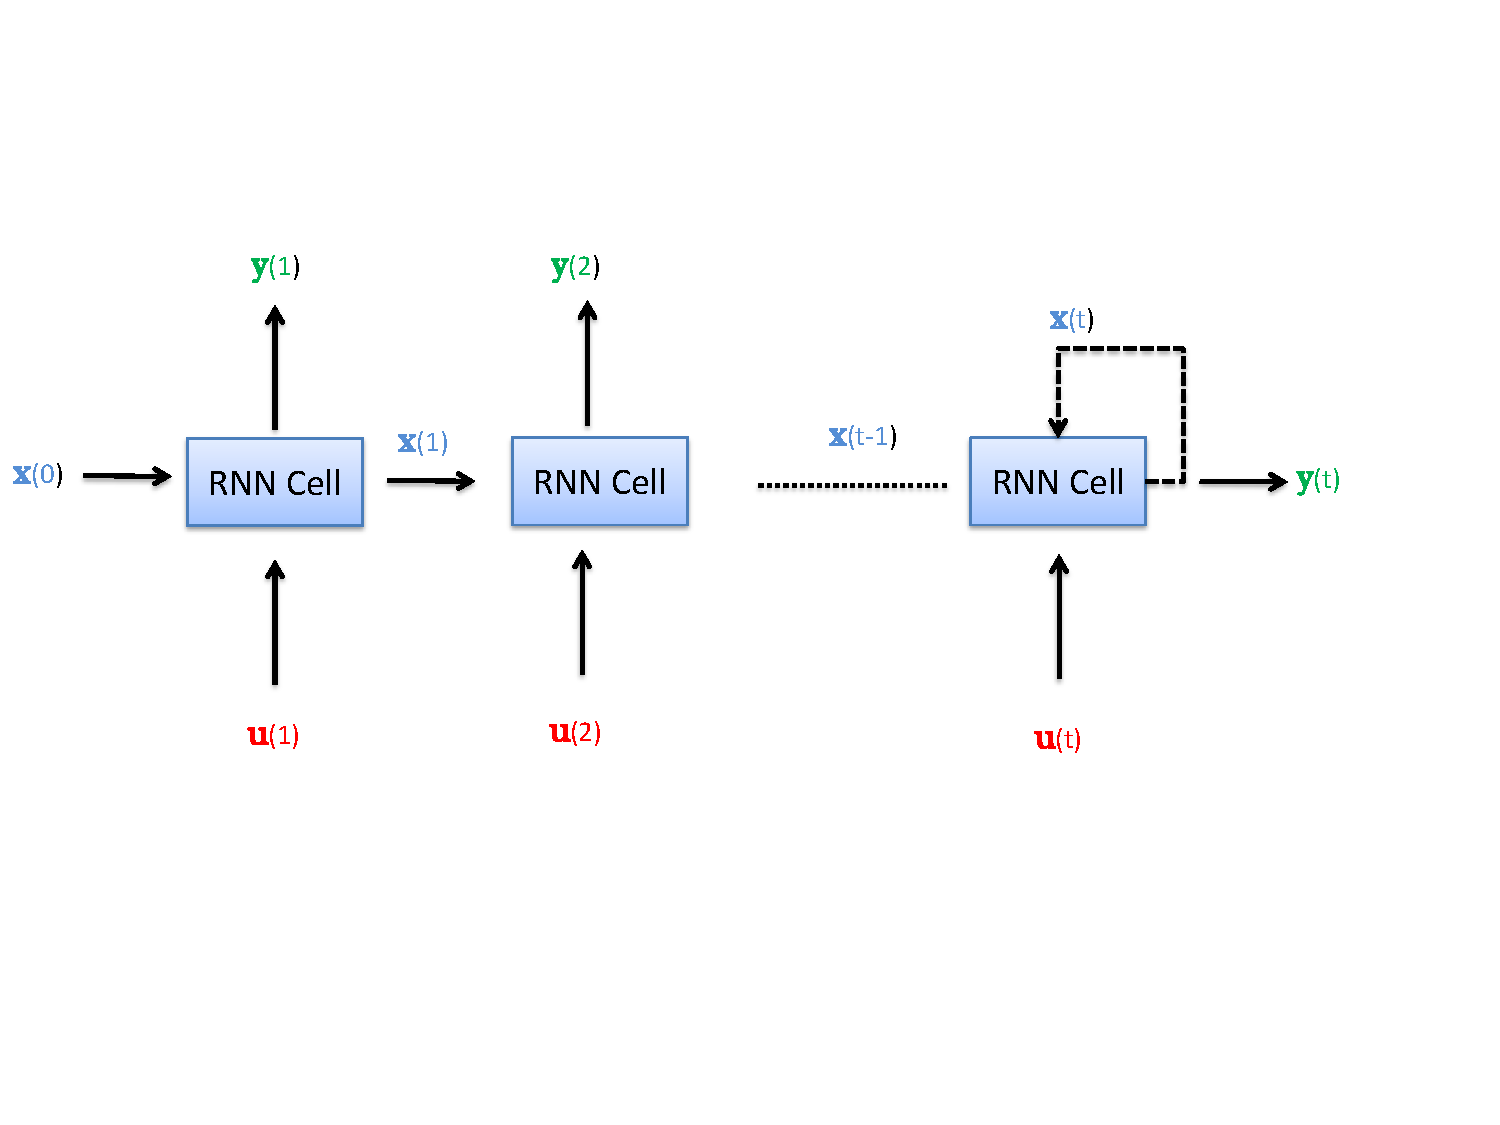
\includegraphics[width=\linewidth]{./Figure/RNN.pdf}
%  \caption{Schematic of a RNN. The recurrent connections in the hidden layer allow information to persist from one input to another. The arrow shows the information flow.}
%  \label{fig:RNN_cell}
% \end{figure}

\begin{figure}[H]
\centering
\begin{tikzpicture}[item/.style={circle,draw,thick,align=center},
itemc/.style={item,on chain,join}]
 \begin{scope}[start chain=going right,nodes=itemc,every
 join/.style={-latex,very thick},local bounding box=chain]
 \path node (A0) {\small RNN Cell} node (A1) {\small RNN Cell} node (A2) {\small RNN Cell} node[xshift=2em] (At)
 {\small RNN Cell};
 \end{scope}
 \node[left=1em of chain,scale=2] (eq) {$=$};
 \node[left=2em of eq,item] (AL) {RNN Cell};
 \path (AL.west) ++ (-1em,2em) coordinate (aux);
 \draw[very thick,-latex,rounded corners] (AL.east) -| ++ (1em,2em) -- (aux) 
 |- (AL.west);
 \foreach \X in {0,1,2,t} 
 {\draw[very thick,-latex] (A\X.north) -- ++ (0,2em)
 node[above,item,fill=gray!10] (h\X) {$y(\X)$};
 \draw[very thick,latex-] (A\X.south) -- ++ (0,-2em)
 node[below,item,fill=gray!10] (x\X) {$u(\X)$};}
 \draw[white,line width=0.8ex] (AL.north) -- ++ (0,1.9em);
 \draw[very thick,-latex] (AL.north) -- ++ (0,2em)
 node[above,item,fill=gray!10] {$y(t)$};
 \draw[very thick,latex-] (AL.south) -- ++ (0,-2em)
 node[below,item,fill=gray!10] {$u(t)$};
 \path (x2) -- (xt) node[midway,scale=2,font=\bfseries] {\dots};
\end{tikzpicture}
 \caption{Schematic of a RNN. The recurrent connections in the hidden layer allow information to persist from one input to another. The arrow indicate the information flow.}
 \label{fig:RNN_cell}
\end{figure}

where $x(n-1)$ is the recurrent hidden state, which represents the a state in the past. $\mathbf{\Theta}^{in}$, $\mathbf{\Theta}$ and $b$ are the input-hidden and hidden-hidden weight matrices and a bias vector. $f$ is a non-linear activation function, usually a sigmoid or hyperbolic tangent. The initial hidden state $x(0)$ is determined by the experimenter, usually initialized  to zero or random~\cite{pascanu2013difficulty}. The output at any time $n$ is computed as follows:

\begin{equation}
\mathbf{y}(n) = f(\mathbf{\Theta}^{out} x(n))
\label{equ:rnn_out}
\end{equation}

where $\mathbf{\Theta}^{out}$ is the hidden-output weight matrices.


One approach of training RNNs (i.e. learning optimal weights for a given task) is through back-propagation through time (BPTT)~\cite{Rumelhart:1986:LIR:104279.104293,rumelhart1986learning}, where the RNN is unfolded through time and represented as a feed-forward network (with an unbounded number of layers) and back-propagation is applied on the unrolled RNN as shown in Figure~\ref{fig:RNN_cell}.

However as discussed in Section~\ref{sec: Introduction_to_sequence_model}, RNNs are enable to capture long-term time dependencies (i.e. remembering state of longer sequences), this is due to the gradient information either decays or  explodes exponentially during training. These phenomenons are called the vanishing and exploding gradients and are well studied in RNNs problem~\cite{pascanu2013difficulty}. The exploding gradient problem refers to the large increase in the norm (i.e magnitude) of the gradient during training, such that long-term time dependencies grow exponentially more than short-term ones from one RNN cell state to another. In contrast to the vanishing gradient problem, where long-term time dependencies decrease exponentially to magnitude close to zero, making it diffult to training RNNs to learn correlation between temporal distant events.


Therefore, this concludes that RNNs are not be suitable for problems that require long-term memory (i.e. speech processing, text and video summarization..etc), making the suffer from short-term memory.

% \subsection{Exploding and vanishing gradients}
% \label{sec:Exploding_and_vanishing_gradients}

\subsection{Long short-term memory (LSTM)}
\label{sec:Long_Short_Term_Memory}
In order to address RNNs inability to deal with problems that require long-term memory, Long Short-Term Memory (LSTM) was proposed in 1997 by Sepp Hochreiter and Jurgen Schmidhuber~\cite{schmidhuber1992fixed}. Fundamentally the difference between RNNs and LSTMs is in their ability to capture long-term memory, and this is due to the gating mechanism in LSTMs, and this is what sets then apart from RNNs. These gating mechanisms solves the short-term memory problem of RNNs. 


Consider the LSTM cell in Figure~\ref{fig:lstm}, at each time step $n$, three inputs are given to the LSTM cell, the current input signal $\mathbf{u}(n)$, the short-term memory from the previous LSTM cell the \textit{hidden state}  $\mathbf{x}(n-1)$ and the long-term memory $\mathbf{c}(n-1)$ the \textit{cell state}.

Before passing on the long-term and short-term memory from one LSTM cell to another, the gates in control the flow of information that is important to keep and redundant to discard at each time step $n$ 

% The LSTM cell uses gates to control the flow of information that needs to be kept or discarded at each time step $n$ before passing on the long-term and short-term information to the next LSTM cell. Intuitively if we follow the analogue that these gate represent water filters. Then the role of these gates is supposed to selectively remove any irrelevant information, similar to how water filter prevents impurities from passing through. At the same time, only water and beneficial nutrients can pass through these filters, just like how gates only hold on to useful information.

The most common architecture described is used in this thesis~\cite{graves2012supervised}. Consider a LSTM cell as shown in Figure~\ref{fig:lstm} with three gates: an input gate $i$,  forget gate $f$, and an output gate $o$, which updates the  memory $c$ at any time $n$.

\begin{figure}[H]
\centering
\begin{tikzpicture}[
    % GLOBAL CFG
    font=\sf \scriptsize,
    >=LaTeX,
    % Styles
    cell/.style={% For the main box
        rectangle, 
        rounded corners=5mm, 
        draw,
        very thick,
        },
    operator/.style={%For operators like +  and  x
        circle,
        draw,
        inner sep=-0.5pt,
        minimum height =.2cm,
        },
    function/.style={%For functions
        ellipse,
        draw,
        inner sep=1pt
        },
    ct/.style={% For external inputs and outputs
        circle,
        draw,
        line width = .75pt,
        minimum width=1cm,
        inner sep=1pt,
        },
    gt/.style={% For internal inputs
        rectangle,
        draw,
        minimum width=4mm,
        minimum height=3mm,
        inner sep=1pt
        },
    mylabel/.style={% something new that I have learned
        font=\scriptsize\sffamily
        },
    ArrowC1/.style={% Arrows with rounded corners
        rounded corners=.25cm,
        thick,
        },
    ArrowC2/.style={% Arrows with big rounded corners
        rounded corners=.5cm,
        thick,
        },
    ]

%Start drawing the thing...    
    % Draw the cell: 
    \node [cell, minimum height =4cm, minimum width=6cm] at (0,0){} ;

    % Draw inputs named ibox#
    \node [gt] (ibox1) at (-2,-0.75) {$f$};
    \node [gt] (ibox2) at (-1.5,-0.75) {$f$};
    \node [gt, minimum width=1cm] (ibox3) at (-0.5,-0.75) {Tanh};
    \node [gt] (ibox4) at (0.5,-0.75) {$f$};

  % Draw opérators   named mux# , add# and func#
    \node [operator] (mux1) at (-2,1.5) {$\times$};
    \node [operator] (add1) at (-0.5,1.5) {+};
    \node [operator] (mux2) at (-0.5,0) {$\times$};
    \node [operator] (mux3) at (1.5,0) {$\times$};
    \node [function] (func1) at (1.5,0.75) {Tanh};

    % Draw External inputs? named as basis c,h,x
    \node[ct, label={[mylabel]Cell State (long-term memory)}] (c) at (-6,1.5) {$\mathbf{c}(n-1)$};
    \node[ct, label={[mylabel] Hidden State (short-term memory)}] (h) at (-6,-1.5) {$\mathbf{x}(n-1)$};
    \node[ct, label={[mylabel]left:Input}] (x) at (-2.5,-3) {$\mathbf{u}(n)$};

    % Draw External outputs? named as basis c2,h2,x2
    \node[ct, label={[mylabel]new cell state}] (c2) at (5,1.5) {$\mathbf{c}(n)$};
    \node[ct, label={[mylabel]new hidden state}] (h2) at (5,-1.5) {$\mathbf{x}(t)$};
    \node[ct, label={[mylabel]left:Output}] (x2) at (2.5,3) {$\mathbf{y}(n)$};

% Start connecting all.
    %Intersections and displacements are used. 
    % Drawing arrows    
    \draw [ArrowC1] (c) -- (mux1) -- (add1) -- (c2);

    % Inputs
    \draw [ArrowC2] (h) -| (ibox4);
    \draw [ArrowC1] (h -| ibox1)++(-0.5,0) -| (ibox1); 
    \draw [ArrowC1] (h -| ibox2)++(-0.5,0) -| (ibox2);
    \draw [ArrowC1] (h -| ibox3)++(-0.5,0) -| (ibox3);
    \draw [ArrowC1] (x) -- (x |- h)-| (ibox3);

    % Internal
    \draw [->, ArrowC2] (ibox1) -- (mux1);
    \draw [->, ArrowC2] (ibox2) |- (mux2);
    \draw [->, ArrowC2] (ibox3) -- (mux2);
    \draw [->, ArrowC2] (ibox4) |- (mux3);
    \draw [->, ArrowC2] (mux2) -- (add1);
    \draw [->, ArrowC1] (add1 -| func1)++(-0.5,0) -| (func1);
    \draw [->, ArrowC2] (func1) -- (mux3);

    %Outputs
    \draw [-, ArrowC2] (mux3) |- (h2);
    \draw (c2 -| x2) ++(0,-0.1) coordinate (i1);
    \draw [-, ArrowC2] (h2 -| x2)++(-0.5,0) -| (i1);
    \draw [-, ArrowC2] (i1)++(0,0.2) -- (x2);
\end{tikzpicture}
\caption{Schematic of an Long Short-Term Memory Cell. }
\label{fig:lstm}
\end{figure}

The input gate determines which new state to be stored in the long-term memory $\mathbf{c}$. given the current input signal $\mathbf{u}(n)$  and the previous hidden state $\mathbf{x}(n-1)$, a sigmoid function $f$ is applied to give values in the range \[0,1\], where values close to 0 indicate discarded states and 1 states that will be kept for the next step. Back-propagation is applied in this layer in order to learn  which states to kept or remove. The state are computed as follows,

% The input gate decides what new information will be stored in the long-term memory $\mathbf{c}$. Given the the current input signal $\mathbf{u}(n)$ and the previous hidden state $\mathbf{x}(n-1)$, this gate consist of 2 layers. To create this layer, we pass the hidden state $\mathbf{x}(n-1)$ and the current input signal $\mathbf{u}(n)$ into a sigmoid function $f$. The sigmoid function transforms the values in the range of 0 and 1, with 0 indicating that part of the information is unimportant, whereas 1 indicates that the information will be kept. This helps to decide the values to be kept and used, and also the values to be discarded. As the layer is being trained through back-propagation, the weights in the sigmoid function will be updated such that it learns to only let the useful pass through while discarding the less critical features. And are computed as follows, 

\begin{equation}
i_{1} = f(\mathbf{\Theta}^{in}_{i_{1}} (\mathbf{x}(n-1),\mathbf{u}(n) ) + b_{i_{1}} )
\end{equation}

In the second layer a $tanh$ function is applied to $\mathbf{x}(n-1)$ and $\mathbf{u}(n)$.
\begin{equation}
i_{2} = tanh(\mathbf{\Theta}^{in}_{i_{2}} (\mathbf{x}(n-1),\mathbf{u}(n) ) + b_{i_{2}} )
\end{equation}

Multiply the output from the previous 2 layers determines which states are to be kept in the long-term memory, and is computed as follows,
% The outputs from these 2 layers are then multiplied, and the final outcome represents the information to be kept in the long-term memory and used as the output, and is computed as follows, 
\begin{equation}
i_{input} = i_{1} \times i_{2}
\end{equation}

The forget gate decides which information from the long-term memory should be kept or discarded, and it computed as follow,

\begin{equation}
i_{forget} = f(\mathbf{\Theta}^{in}_{i_{forget}} (\mathbf{x}(n-1),\mathbf{u}(n) ) + b_{i_{forget}} )
\end{equation}

 This new long-term memory is computed as follows,

\begin{equation}
\mathbf{c}(n) = \mathbf{c}(n-1) \times i_{forget} + i_{input}
\end{equation}

The output gate will take the current input, the previous short-term memory, and the newly computed long-term memory to produce the new short-term memory/hidden state which will be passed on to the cell in the next time step $n$. Computed as follows,

\begin{equation}
y_{1} = f(\mathbf{\Theta}^{in}_{o_{1}} (\mathbf{x}(n-1),\mathbf{u}(n) ) + b_{o_{1}} )
\end{equation}

\begin{equation}
y_{2} = tanh(\mathbf{\Theta}^{in}_{o_{2}} \mathbf{c}(n) + b_{o_{2}} )
\end{equation}

\begin{equation}
y(n) = y_{1} \times y_{2}
\end{equation}

The short-term and long-term memory produced by these gates will then be carried over to the next LSTM cell. The output of each time step can be obtained from the short-term memory, also known as the hidden state. However, these gating mechanisms in LSTM increase the number of parameters to be learned and therefore require a lot of computational memory to train and also take longer to train.

\subsection{Gated Recurrent Unit (GRU)}
\label{sec:gated_recurrent_unit}
Gated Recurrent Units (GRUs) is another variate RNN, introduced in 2014 by Kyunghyun et al~\cite{bahdanau2014neural} to solve the vashining and exploding gradients during back-propagation thought time. Similar to LSTMs, GRUs also use gating mechanism to control the flow of information between cell~\footnote{cell are object with a single scalar output}, while LSTMs have two different states passed across cells, the cell and hidden state, GRUs only have one the hidden state, this makes them have less parameters to learn, which means they train faster and require less computational memory that LSTMs. The architecture in the gates in GRUs enable the hidden state to capture both long-term and short-term memory.


Consider the GRU cell in Figure~\ref{fig:gru}, at each time step $n$, the cell takes two different inputs, the current input signal $\mathbf{u}(n)$ and the previous hidden state $\mathbf{x}(n-1)$. The GRUs consist of two fundamental gates, the update $z$ gate and the reset gate $r$. The updated gate acts similar to the forget and input gate in LSTMs, it decide what  information to discard and what new information to keep. The update is computed as follows,

\begin{equation}
\mathbf{z}(n) = \sigma (\mathbf{\Theta}^{in}_{z} \mathbf{u}(n) + \mathbf{\Theta}_{z} \mathbf{x}(n-1))
\label{equ:update_gate}
\end{equation}


where $\mathbf{\Theta}^{in}_{z} , \mathbf{\Theta}_{z}$ are the input and internal weights respectively in the updated gate. The reset gate decides how much past information to forget and it is updated as follows,

\begin{equation}
\mathbf{r}(n) = \sigma (\mathbf{\Theta}^{in}_{r} \mathbf{u}(n) + \mathbf{\Theta}_{r} \mathbf{x}(n-1))
\label{equ:reset_gate}
\end{equation}


where $\mathbf{\Theta}^{in}_{r} , \mathbf{\Theta}_{r}$ are the input and internal weights respectively in the reset gate.  And lastly, $tanh$ is applied to results in Equation~\ref{equ:reset_gate} such that,


\begin{equation}
\mathbf{\Tilde{r}}(n) = tanh (\mathbf{\Theta}^{in} \mathbf{u}(n) + \mathbf{\Theta} ( \mathbf{r}(n-1) \mathbf{x}(n-1)   )
\label{equ:reset_gate2}
\end{equation}

The linear combination between the previous activation $\mathbf{x}(n-1)$  and $\mathbf{\Tilde{r}}(n)$ is the new hidden state, and it is computed as follows, 

\begin{equation}
\mathbf{x}(n) = (1-\mathbf{z}(n)\mathbf{x}(n-1)) + \mathbf{z}(n)\mathbf{\Tilde{r}}(n) 
\label{equ:gru_final_activation}
\end{equation}



\begin{figure}[H]
\centering
\begin{tikzpicture}[
    % GLOBAL CFG
    font=\sf \scriptsize,
    >=LaTeX,
    % Styles
    cell/.style={% For the main box
        rectangle, 
        rounded corners=5mm, 
        draw,
        very thick,
        },
    operator/.style={%For operators like +  and  x
        circle,
        draw,
        inner sep=-0.5pt,
        minimum height =.2cm,
        },
    function/.style={%For functions
        ellipse,
        draw,
        inner sep=1pt
        },
    ct/.style={% For external inputs and outputs
        circle,
        draw,
        line width = .75pt,
        minimum width=1cm,
        inner sep=1pt,
        },
    gt/.style={% For internal inputs
        rectangle,
        draw,
        minimum width=4mm,
        minimum height=3mm,
        inner sep=1pt
        },
    mylabel/.style={% something new that I have learned
        font=\scriptsize\sffamily
        },
    ArrowC1/.style={% Arrows with rounded corners
        rounded corners=.25cm,
        thick,
        },
    ArrowC2/.style={% Arrows with big rounded corners
        rounded corners=.5cm,
        thick,
        },
    ]

%Start drawing the thing...    
    % Draw the cell: 
    \node [cell, minimum height =4cm, minimum width=6cm] at (0,0){} ;

    % Draw inputs named ibox#
    \node [gt] (ibox1) at (-2,-0.75) {$f$};
    \node [gt] (ibox2) at (-1.5,-0.75) {$f$};
    \node [gt, minimum width=1cm] (ibox3) at (-0.5,-0.75) {Tanh};
    \node [gt] (ibox4) at (0.5,-0.75) {$f$};

  % Draw opérators   named mux# , add# and func#
    \node [operator] (mux1) at (-2,1.5) {$\times$};
    \node [operator] (add1) at (-0.5,1.5) {+};
    \node [operator] (mux2) at (-0.5,0) {$\times$};
    \node [operator] (mux3) at (1.5,0) {$\times$};
    \node [function] (func1) at (1.5,0.75) {Tanh};

    % Draw External inputs? named as basis c,h,x
    \node[ct, label={[mylabel]Cell State (long-term memory)}] (c) at (-6,1.5) {$\mathbf{c}(n-1)$};
    
    % \node[ct, label={[mylabel] Hidden State (short-term memory)}] (h) at (-6,-1.5) {\mathbf{x}(n-1)};
    
    \node[ct, label={[mylabel]left:Input}] (x) at (-2.5,-3) {$\mathbf{u}(n)$};

    % Draw External outputs? named as basis c2,h2,x2
    \node[ct, label={[mylabel]new cell state}] (c2) at (5,1.5) {$\mathbf{c}(n)$};
    
    % \node[ct, label={[mylabel]new hidden state}] (h2) at (5,-1.5) {\mathbf{x}(t)};
    
    % \node[ct, label={[mylabel]left:Output}] (x2) at (2.5,3) {\mathbf{y}(n)};

% Start connecting all.
    %Intersections and displacements are used. 
    % Drawing arrows    
    \draw [ArrowC1] (c) -- (mux1) -- (add1) -- (c2);

    % Inputs
    \draw [ArrowC2] (h) -| (ibox4);
    \draw [ArrowC1] (h -| ibox1)++(-0.5,0) -| (ibox1); 
    \draw [ArrowC1] (h -| ibox2)++(-0.5,0) -| (ibox2);
    \draw [ArrowC1] (h -| ibox3)++(-0.5,0) -| (ibox3);
    \draw [ArrowC1] (x) -- (x |- h)-| (ibox3);

    % Internal
    \draw [->, ArrowC2] (ibox1) -- (mux1);
    \draw [->, ArrowC2] (ibox2) |- (mux2);
    \draw [->, ArrowC2] (ibox3) -- (mux2);
    \draw [->, ArrowC2] (ibox4) |- (mux3);
    \draw [->, ArrowC2] (mux2) -- (add1);
    \draw [->, ArrowC1] (add1 -| func1)++(-0.5,0) -| (func1);
    \draw [->, ArrowC2] (func1) -- (mux3);

    %Outputs
    \draw [-, ArrowC2] (mux3) |- (h2);
    \draw (c2 -| x2) ++(0,-0.1) coordinate (i1);
    \draw [-, ArrowC2] (h2 -| x2)++(-0.5,0) -| (i1);
    \draw [-, ArrowC2] (i1)++(0,0.2) -- (x2);
\end{tikzpicture}
\caption{Schematic of an Gated Recurrent Memory Cell. }
\label{fig:gru}
\end{figure}


GRUs are faster and require less computational memory to train than LSTMs. However, LSTMs in terms of cases where performance crucial over the computational cost, LSTMs remain state  of the art in long-term memory problems. 

\subsection{Conclusion}
\label{sec:RNNs_conclusion}

The fundamental distinction between regular RNNs and LSTMs/GRUs is that the latter support gating of the hidden state, this gates determine when and how the hidden state is updated. 

Standard RNNs and LSTMs/GRUs still remain powerful tools for modeling sequential data, however training these models is computationally expensive and unstable during the optimization of  larger hidden weights through back-propagation~\cite{jaeger2003adaptive}. Therefore an cheaper and efficient alternative is required for training RNNs. 

\newpage
% \subsection{Various types of RNNs}
% \label{sec:Various_types_of_RNNs}
% \newpage
\section{Reservoir Computing (RC)}
\label{sec:Reservoir_Computing}
\subsection{Introduction}
Reservoir computing (RC) is a neural network-based computing paradigm that allows efficient processing of time-varying inputs~\cite{du2017reservoir}. RC introduces a dynamic \textit{reservoir} having a short-term memory~\footnote{short-term memory is when the current outputs $y(n)$ depends on earlier values of the input $u(n-k)$ and/or earlier values from the outputs it self $y(n-k)$.} to project features from the temporal inputs into a high-dimensional feature space. A \textit{readout} function layer is used to learn the projected features for any problems, such as classification and regression. RC systems can efficiently capture auto-correlated events within the data, and training such systems is computationally cheap, since only the \textit{readout} layer is trained using a linear method. Both the online (e.g., gradient descent) and offline methods (closed form linear regression) \textit{readout} layer can be used to train the read layer~\cite{DBLP:journals/corr/GoudarziMBFTS16}..


% since only the \textit{readout} layer needs to be trained in a linear fashion. The linear readout layer can either be trained by a online (e.g., gradient descent) or offline  methods (e.g., closed-form linear regression or determined analytically in certain cases)~\cite{DBLP:journals/corr/GoudarziMBFTS16}.

\subsection{Formalism}
\label{sec:Formalism}


Consider a temporal task~\footnote{A temporal task is where $\mathbf{u}(n)$ and $\mathbf{y}_{target}(n)$ are signals in a discrete time domain $n = 1,...N$, and $N$ , and the goal is to learn a function $\mathbf{y} = y(...,\mathbf{u}(n-1),\mathbf{u}(n))$ such that  $E(\mathbf{y}, \mathbf{y}_{target})$ is minimized} of learning a functional relation $f$ between a discrete time input signal $\mathbf{u}(n)$ and a discrete time target output $\mathbf{y}_{target}(n)$ such that the error $E (\mathbf{y}, \mathbf{y}_{target})$ is minimized. Then the learned output $\mathbf{y}$ will be given by,

\begin{equation}
\mathbf{y}(n) = f( ...,\mathbf{u}(n-1), \mathbf{u}(n))
\label{equ:Temporal_task_problem}
\end{equation}


where $n = 1,...N$, and $N$ is the number of examples in the training dataset $\{(\mathbf{u}(n),\mathbf{y}_{target}(n))\}$.

Most problems are non-linear, and cannot be easily solved using a simple linear relationship between the input $\mathbf{u}(n)$ and output $\mathbf{y}(n)$ signal, in the form,

\begin{equation}
\mathbf{y}(n) = \mathbf{{\Theta}^{out}} \hspace{0.2em} \mathbf{x}(n)
\label{equ:Linear_model}
\end{equation}

where $\mathbf{{\Theta}^{out}}$ and $\mathbf{x}(n)$ are the output (i.e learned) weights and the reservoirs activation's, respectively. This is because the error $E(\mathbf{y}, \mathbf{y}_{target})$ is big regardless of $\mathbf{{\Theta}^{out}}$.

Using the reservoir $\mathbf{x}(n)$ to spatially transforms the input signals history $\mathbf{u}(n)$, one can resort in the expansion of the input signal $u(n)$ into a high-dimensional feature vector $\mathbf{u}(n) \in R^{N_{u}} $, and this feature vector serves a transformed (i.e new) input that is used by a linear method. This approach is referred to as a \textit{kernel} method with a called kernel function $K$, then $\mathbf{x}(n)$ is in the form,


\begin{equation}
\mathbf{x}(n) =  K(\mathbf{u}(n))
\label{equ:kernel_expansion}
\end{equation}


The function to be learned in any temporal task depends on the history of the input signal,

\begin{equation}
\mathbf{x}(n) = K(...,\mathbf{u}(n-1),\mathbf{u}(n))
\label{equ: Kernel_memory_expansion}
\end{equation}


and returns the high dimensional current input signal and its potentially infinite history~\cite{lukovsevivcius2009reservoir}. $K$  has the potential of having an infinite number of parameters, practical implementations normally require the function to be defined recursively as,

\begin{equation}
\mathbf{x}(n) = K(\mathbf{x}(n-1),\mathbf{u}(n))
\label{equ: Kernel_recursive_expansion}
\end{equation}

We can then use $\mathbf{x}(n)$ and a linear method in Equation~\ref{equ:Linear_model} to approximate $\mathbf{y}(n)$, as follows,

\begin{equation}
\begin{aligned}
\mathbf{y}(n) &= \mathbf{{\Theta}^{out}} \hspace{0.2em} \mathbf{x}(n)\\
&=\mathbf{{\Theta}^{out}}\hspace{0.2em} K(\mathbf{x}(n-1),\mathbf{u}(n))
\label{equ:Kernel_expansion_readout}
\end{aligned}
\end{equation}


The purpose of learning  $\mathbf{y}(n)$  is then to find the output weights $\mathbf{{\Theta}^{out}}$ that minimize the error $E (\mathbf{y}, \mathbf{y}_{target})$. It is important to state that the $K$ function of Equations~\ref{equ: Kernel_memory_expansion} and~\ref{equ: Kernel_recursive_expansion} represents a dynamic system driven by the input signal $\mathbf{u}(n)$.

This method, along with several main streams of RC are described in more details below.


\subsection{Echo state networks (ESNs)}
\label{sec:Echo_State_Networks}


In 2001, a fundamentally new approach to RNN design and training was proposed by Jaeger et al. (2001) under the name of \textit{Echo State Networks}~\cite{jaeger2001echo}. The echo state approach is based on the observation that if the RNN is randomly initialized, then the training of the linear readouts is adequate to achieve excellent performance in practical applications with a simple model~\cite{lukovsevivcius2009reservoir}. The untrained part of the RNN is referred as a \textit{reservoir} \footnote{The reservoir is similiar to the hidden layer in RNNs.} and the resulting activated reservoir states $\mathbf{x}(t)$ are referred to as the \textit{echoes} of the input history as shown in Figure~\ref{fig:reservoir_computing}.

\begin{definition}
\emph{(Echo State Network )}
Echo State Network is a recurrent and random sigmoidal neural network which is driven by an input signal in the discrete time \footnote{discrete time refers to the discrete nature of sequences (i.e. they are made of data indexed by integers)}, and the activations of the neurons are treated with a linear method. The reservoir acts as a complex non-linear dynamic filter that transforms input signals using a highly dimensional temporal map~\cite{jaeger2001echo}.
\label{def:Echo_State_Network}
\end{definition}



\begin{figure}[H]
\begin{center}
\begin{tikzpicture}[node distance = 1.5cm, thick, nodes = {align = center},>=latex]
% Input nodes
\node[place] (A) {$u_{0}$};
\node[place] (B) [below of=A]  {$u_{1}$};
\node[place] (C) [below of=B]  {$u_{2}$};
\node[dot] (D) [below of=C] {};
\node[place] (E) [below of=D]  {$u_{N_{u}}$};
\node (inn)[above of=A] {\color{red} $N_{u}$ input units}; 
\node[rectangle, draw=black,draw=red!60, fit=(A) (B) (C) (D) (E) , inner sep=1mm] (all) {};

% Reservoir nodes
\node[place] (r1) [below right=0.cm and 5cm of A] {$x_{0}$};
\node[place] (r2) [below right=0.6cm and 0.5cm of r1] {$x_{1}$};
\node[place] (r3) [below right=0.6cm and 5cm of D] {$x_{2}$};
\node[place] (r4) [above left=0.3cm and 1cm of r3] {$x_{N_{x}}$};
\node (rr) [ right=1cm of inn] { \color{blue} $N_{x}$ internal reservoir units  }; 
\draw [black,thick,->] (r1) to node[right] {$ {\theta}_{0,1} $}  (r2) ;
\draw [black,dotted,->] (r2) -- node[right] {$ {\theta}_{1,N_{x}} $} (r4);
\draw [black,dotted,->] (r2) -- node[right] {${\theta}$} (r4);
\draw [black,thick,->] (r3) to [out=90,in=180] node[right] {$ {\theta}_{2,0} $} (r1);
\draw [black,dotted,->] (r4) to [out=180,in=180] node[right] {$ {\theta}_{N_{x},0} $}(r1);
\draw[black,thick,->] (r3.-90)  arc (180:180+264:4mm) ;
\node[circle, draw=black,draw=blue!60, fit=(r1) (r2) (r3) (r4), inner sep=0.5mm] (reser) {};
%Output node
%\node[place] (o1)  [right=2cm of reser] {}; % Input nodes
\node[place] (o1)  [right=9cm of A] {$y_{0}$}; % Input nodes
\node[place] (o2)  [below of=o1] {$y_{1}$};
\node[place] (o3)  [below of=o2] {$y_{1}$};
\node[dot] (o4)  [below of=o3] {};
\node[place] (o5)  [below of=o4]  {$y_{N_{y}}$};
\node  [right =7cm  of inn] { \color{green} $N_{y}$ output units}; 
\node[rectangle, draw=black,draw=green!60, fit=(o1) (o2) (o3) (o4) (o5), inner sep=1mm] (all3) {};

\draw [black,thick,->] (A) to node[above]{$ {\theta^{in}}_{n,n} $} (reser);
\draw [black,thick,->] (B) to node[above] {$ {\theta^{in}}_{n,1} $} (reser);
\draw [black,thick,->] (C) to node[above] {$ {\theta^{in}}_{n,2} $} (reser);
\draw [black,dotted,->] (E) to node[above] {$ {\theta^{in}}_{N_{x},N_{u}} $} (reser);

\draw [black,thick,->] (reser) to node[above] {$ {\theta^{out}}_{0,n} $} (o1);
\draw [black,thick,->] (reser) to node[above] {$ {\theta^{out}}_{1,n} $} (o2);
\draw [black,thick,->] (reser) to node[above] {$ {\theta^{out}}_{2,n} $} (o3);
\draw [black,dotted,->] (reser) to node[above] {$ {\theta^{out}}_{N_{y},N_{y}} $} (o5);
\end{tikzpicture}
\end{center}
\caption{Schematic of an Echo State Network. }
\label{fig:reservoir_computing}
\end{figure}


This new approach aims to overcome the shortcomings of RNN training mentioned in Section~\ref{sec:Introduction}, by setting up RNNs in the as follows:
\begin{itemize}
%\item A RNN is randomly created and remains unchanged during training, this RNN is called the \textit{reservoir}.
\item The RNN is created with random dynamic parameters and connections.
\item The reservoir acts as a complex, high-dimensional, non-linear dynamical system.
\item The reservoir is excited by the input and maintains in its state a non-linear transformation of the entire input history.
\item The reservoir has to be exponentially stable (i.e. fading memory over time).
% \item The target output signal is generated as a linear combination of the neuron's signal from the input-driven reservoir.
\item A linear combination of the input-reservoir signals are used to compute the target output signal.
\item Optimal output weights can be learned using linear methods (e.g., regression ) as as shown in Figure~\ref{fig:reservoir_computing}
% \item Output weights can be learned using a regression as shown in Figure~\ref{fig:reservoir_computing}
\label{item:New_RRN_approach}
\end{itemize}



Consider the ESN shown in Figure~\ref{fig:reservoir_computing}, which is derived directly from Equation~\ref{equ: Kernel_recursive_expansion}. The reservoir of the ESN is exited by input signal $\textbf{u}(n)$ with $N_{u}$ input neurons, and the corresponding activations of $N_{x}$ neurons in the reservoir at any time $n$ are given by,

\begin{equation}
\textbf{x}(n) = (x_{1}(n),...,x_{N_{x}}(n))^{T}
\label{equ:state_vector}
\end{equation}

similarly, the output activations or readouts $\textbf{y}(n)$ of $N_{y}$ neurons in the output layer at any time $n$ are given as,

\begin{equation}
\textbf{y}(n) = (y_{1}(n),...,y_{N_{y}}(n))^{T} 
\label{equ:output_vector}
\end{equation}

where $\mathbf{\Theta}^{in}$ are the input-reservoir connections, $\mathbf{\Theta}$ recurrent connections in the reservoir and $\mathbf{\Theta}^{out}$ are the reservoir-output connections , respectively  defined as follows,

\begin{eqnarray}
{\mathbf{\Theta}}^{in} &= ({\theta}^{in}_{1},...,{\theta}^{in}_{N_{u}})^{T} \\
{\mathbf{\Theta}} =& ({\theta}_{1},...,{\theta}_{N_{x}})^{T}\\
{\mathbf{\Theta}}^{out} &= ({\theta}^{out}_{1},...,{\theta}^{out}_{N_{y}})^{T}
\label{equ:weight_vectors}
\end{eqnarray}


When the feedback from the output to reservoir is not considered. The temporal neural state in the reservoir is described as follows,
 
 \begin{equation}
\mathbf{x}(n) =
f({(1-\tau)\mathbf{x}(n-1)  + \tau(\mathbf{\Theta}}^{in} \mathbf{u}(n) + \alpha{\mathbf{\Theta}} \mathbf{x}(n-1) +  \mathbf{\lambda}(n)) )
\label{equ:reservoir_activations}
\end{equation}
 
where $n$ denote the discrete time, $\tau$ is the  leaking rate, $\alpha$ is the spectral radius and ${\lambda}(n)$ is a regularization parameter (noise term) and  $f$ is a nonlinear activation function, usually the symmetric $tanh$, or the positive sigmoid~\cite{lukovsevivcius2009reservoir}. Equation~\ref{equ:reservoir_activations} represents  a dependent dynamical system (i.e time-dependent dynamical systems) driven by the external input signal $\mathbf{u}(n)$.
 
Then the reservoir acts as a non-linear time expansion function with an output having no memory, this enables the reservoir to learn the output states $\mathbf{y}(n)$~\cite{Schaetti2015}. This implies that RC methods are able to understand, 
 
 \begin{itemize}
 \item  $\mathbf{x}(n)$ : as a vector expanding the history of the input signal $(...,\mathbf{u}(n-1),\mathbf{u}(n))$.
 \item $\mathbf{y}_{target}(n)$ : as a linear combination of reservoir neural state activation $\mathbf{x}(n)$ and the approximated signal to be learned $\mathbf{y}(n)$.
 \label{item:ESN}
 \end{itemize}
 
 
The readouts from the reservoir are linear, where the reservoirs state $\mathbf{x}(n)$ is included as part of the input states $\mathbf{u}(t)$. The outputs are given as linear combination of the neural states of the reservoir, input signal and the output weights expressed as,
 
\begin{equation}
\mathbf{y}(n) = g({\mathbf{\Theta}}^{out}[\textbf{x}(n),\textbf{u}(n)])
\label{equ:output_state}
\end{equation}
 
 
where $g$ is the activation function, usually taken to be the unity and [  ] represents the vertical concatenation of vectors.
 
In supervised learning, the output weights $\mathbf{\Theta}^{out}$ are learned such that the error $E(\mathbf{y}, \mathbf{y}_{target})$ is minimized at a given time~\cite{lukovsevivcius2009reservoir}. The performance of the ESN depends on the configuration of the reservoir. The ability of the ESN to approximate any temporal input, the reservoir should satisfy the \textit{echo state property} stated in Definition~\ref{def: Echo_State_Property}, echo state property states; if the network has been running for very long time (from minus infinity in the definition) the current network state $\mathbf{x}(t)$ is uniquely determined by the history of $\mathbf{u}(n-1)$ and $\mathbf{y}(n-1)$ the input and output respectively~\cite{jaeger2001echo}, which means that the reservoir should not be driven by the initial conditions. It is experimentally observed that the echo state property is satisfied for any input signal if the spectral radius (i.e. the maximum eigenvalue of $\mathbf{\Theta}^{out}$) is adjusted to be smaller than 1.



Detailed discussions of these issue are covered in Sections~\ref{sec:Dynamics_and_reservoir_characteristic}


\subsection{Liquid state machines (LSMs)}
\label{sec:Liquid_State_Machines}

Wolfang Mass et al. (2002)  proposed a reservoir methods under the name of \textit{Liquid State Machines} (LSMs) independently of ESN~\cite{maass2002real}. LSMs originated from a computational neuroscience background, with the main focus of understanding computational properties of neural microcircuits~\cite{Maass:2002:MRC:2968618.2968647,maass2002real,maass2004computational,natschlager2003computer}. The LSM model is founded on the idea of  multiple cycles that form a large complex network making up more than 80\% of all synapses in a neocortical column and shows that multiple outputs can be trained to perform different tasks on the same sequence of states as shown in Figure~\ref{fig: Liquid_state_machine}~\cite{Schaetti2015}.


\begin{figure}[H]
\centering
  \includegraphics[width=\linewidth]{./Figure/LSM.pdf}
\caption{Liquid State Machine. }
\label{fig: Liquid_state_machine}
\end{figure}



\begin{definition}
\emph{(Liquid State Machine)}
A Liquid State Machine is a locally connected network, structured in a
three-dimensional, impulse neuron that is randomly created using biologically-based parameters inspired and excited by sequences of external inputs. The responses of all neurons are projected to the next cortical layer where learning occurs~\cite{maass2002real}.
\label{def:Liquid_State_Machine}
\end{definition}



% \begin{figure}
% \centering
%   \includegraphics[width=\linewidth]{LSM.jpg}
%  \caption{Liquid State Machine~\cite{hazan2013temporal}. }
%  \label{fig: Liquid_state_machine}
% \end{figure}


% \par{=========REPLACE FIGURE MY OWN LATEX VERSION=========:Done}

In the LSMs, the reservoir is referred to as a \textit{Liquid}, following an intuitive analogy of excited states as ripples on the surface of a pool of water~\cite{lukovsevivcius2009reservoir}. Formally, an LSM is defined by the state of the liquid ${\mathbf{u}^{M}}(t)$  at continuous time $t$, where $M$ denotes relation to the liquid state machine. The Liquid activation are in the form,

% \begin{eqnarray}
% I(t) - \frac{V_{l}(t)}{R_{l}} = C_{l} \frac{dV_{l}(t)}{dt} 
% \label{equ:Leaky Integrated Fire neuron}
% \end{eqnarray}

\begin{equation}
\mathbf{u}(t)^{M} = (\mathbf{L}^{M} \mathbf{x})(t) 
\label{equ:liquid_states}
\end{equation}



where $\mathbf{L}^{M}$ denotes a liquid (e.g.,,, dynamical system), $\mathbf{x}(s)$ is the input signal at time $s \leq t$. The output $ \mathbf{y}(t)$ of the network can then be calculated using an output function $f^{M}$ for the target function, given by,

\begin{equation}
\mathbf{y}(t) = f^{M} (\mathbf{u}(t) )
\label{equ:liquid_readouts}
\end{equation}


In literature the terms \textit{reservoir} in ESNs and \textit{liquid} in LSMs are used interchangeably in the context of reservoir computing. Although, several differences between ESNs and LSMs exist:

\begin{itemize}
\item The use of LSMs make a model based on spiking neurons, these neurons use a threshold that once exceeded by the
accumulation of inputs produces a pulse at the output of the neuron. The outputs of them are pulse sequences based on a Poisson process. The ESNs primarily use sigmoid neurons, but they can use other types of neurons.

\item LSMs use a broader set of output type functions. A linear combination is widely used by ESNs, LSMs generally admit outputs in the form of layer networks~\cite{Schaetti2015}.

\item   The internal structure of ESNs is mainly based on a random architecture, while that of LSMs is based on the observation of micro-neocortical columns and has the following structure of biological constraints~\cite{Schaetti2015}. The network nodes are placed on a 3D grid based on microcolumns located in the cortex as shown in Figure~\ref{fig: Liquid_state_machine}.
\label{item:differences}
\end{itemize}


As mentioned, in LSMs the reservoir uses a relatively simple spiking neuron model called the \textit{Leaky Integrate Fire} neuron model. The term 'leaky' is a threshold for which the liquid has a fading memory of the driving input. LSMs with spiking neurons are often difficult to implement and to accurately set up and tune and more expensive to emulates on digital computers than ESN, thus are less used in practice~\cite{lukovsevivcius2009reservoir}.



\subsection{Backpropagation-decorrelation learning rule (BPDC)}
\label{sec:Backpropagation-Decorrelation_Learning_Rule}




\begin{figure}
\centering
  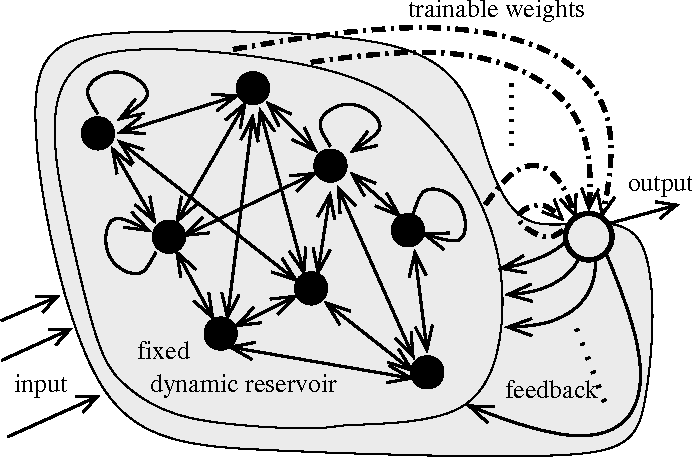
\includegraphics[width=0.8\linewidth]{./Figure/backpropagation_decorrelation.png}
 \caption{Generic Backpropagation-Decorrelation~\cite{steil2006online}. }
 \label{fig:BPDC}
\end{figure}

Two years after the approaches proposed by Jaeger et al. (2001) and Maass et al. (2002), another independent study on recurrent networks has been published under the name of \textit{Backpropagation
-decorrelation} (BPDC) learning rule~\cite{steil2006online}. The BPDC  uses three principles:

\begin{itemize}
    \item single-step back propagation of errors.
    \item the usage of the temporal memory in the network dynamics which is adapted based on decorrelation of the activations.
    \item fixed reservoir of inner neurons to reduce the complexity.
\end{itemize}

% The output weights then implement a linear readout function while at the same time the output neuron provides full feedback into the reservoir.

The readout function is also linear with feedback connection from the output into the reservoir.


In order to derived the BPDC learning rule. Consider a fully connected recurrent network as shown in Figure~\ref{fig:BPDC} excited by external input signal $\mathbf{u}(n)$, then reservoir states $\mathbf{x}(n)$ at any time $n$ are given as,

\begin{equation}
\mathbf{x}(n + \Delta t) = (1-\Delta t)\mathbf{x}(t) + \Delta t \mathbf{\Theta} f(\mathbf{x}(n) + \Delta t \mathbf{\Theta}^{in} \mathbf{u}(n))
\label{equ:backpropagation_decorrelation}
\end{equation}


where $x_{i}, i=1,...,N_{x}$ are the states at time $n<(n+\Delta t)$, $f$ is a activation function, $n$ is discrete time defined as $n= \hat n \Delta t$, $\hat n \in N_{+}$, where $\Delta t$ determines the discrete or continuous dynamics of the reservoir. In order to learn RC using BPDC, the internal neurons must behave as a dynamical reservoir driven by external input $ \mathbf{u}(n)$ which exhibit dynamic memory. Its has a maximal information capacity, that is the states are maximally decorrelated with respect to the given input. Then the output layers can linearly combine these states to readout the desired output.  The weights are updated as follows,



\begin{equation}
\Delta {w_{i,j}}^{BPDC} (n+1) = \frac{\eta}{\Delta t} \frac{f(x_{j}(n)}{\sum_{s} f(x_{s}(n)^{2} + \epsilon} \gamma_{i}(n+1),
\label{equ:backpropagation_decorrelation_weight_update}
\end{equation}

where,

\begin{equation}
\gamma_{i}(n+1)) = \sum_{s \in O} \Big( (1-\Delta t)\delta_{is} + \Delta t w_{is} f'(x_{s}(n)) \Big) e_{s}(n) - e_{i}(n+1),
\label{equ:backpropagation_decorrelation_weight_update_gamma}
\end{equation}



Here $O\subset \{1,...,N_{y}\}$ is a set of indices  $s$  of $N_{y}$ output neurons, $\eta$ is the learning rate, $\epsilon$ the regularization parameter and $e_{s}(n)$ are the non-zero error components for $s\in O$ at time $k$: $e_{s}(n)= x_{s}(n) - y_{s}(n)$ with respect to the desired output signal $y_{s}(n)$. Overtime the output vectors $f(x_{j}(n))$  in Equation~\ref{equ:backpropagation_decorrelation_weight_update} approximates the decorrelation of the neuron output vectors which is imposed by  $\frac{f(x_{j}(n)}{\sum_{s} f(x_{s}(n)^{2} + \epsilon}$~\cite{steil2005memory}. The $\gamma_{i}$ propagate a mixture of the current errors  $e_{s}(n+1)$ and the errors in the last time step  $e_{s}(n)$ weighted by a typical backpropagation term involving $f'$. 


The simplicity of BPDC is due to the fact that the learning rule regarding recurrent learning can be consider as a constraint optimization problem. And the minimization of such as problem the APRL algorithm mentioned in Section~\ref{item: RNN_learning_rules} is used, which revealed that the output weights are quickly adapted while the internal (reservoirs) weights change slowly in RNN training~\cite{lukovsevivcius2009reservoir,Schaetti2015}. BPDC increases the learning times, however, these networks are highly biased to the recent history of the input signal and quickly forget the recent data~\cite{Schaetti2015}.




\subsection{Evolution of recurrent systems with linear output (Evolino)}
\label{sec:Evolution_Of_Recurrent_Systems_With_Linear_Output_(Evolino)}

% Evolino fundamentally extends the idea of ESN from an RNN of a sigmoid unit to a Long Short-Term Memory (LSTM) type of RNNs constructed from units capable of preserving memory for long periods of time, basically, Evolino combines neuroevolution (i.e. the evolution of neural networks) and linear methods (e.g., linear regression) to solve time-dependent problems~\cite{melandriintroduction}. In Evolino the weights of the readouts are trained using evolutionary methods~\cite{lukovsevivcius2009reservoir}. 

Evolino fundamentally extends the idea of short-term memory ESN from a RNN to a LSTM. Evolino combines neuroevolution (i.e. the evolution of neural networks) and linear methods (e.g., linear regression) to solve time-dependent problems~~\cite{melandriintroduction}. The weights of the readouts in Evolino are learned using evolutionary methods~\cite{lukovsevivcius2009reservoir}. 
 

\subsection{Various types of reservoir}
\label{sec:other_types_of_reservoir}
%A variety of neuron models can be used for the reservoir
The reservoir can comprise of different neurons structures. Furthermore, different reservoirs exist due to the different topologies, activation functions used to construct the reservoir. 
Some of which include,  Quantized-ESNs are ESNs whose node states take discrete units, where the number of possible states of a single unit is controlled by a parameter called quantization
level~\cite{schrauwen2009computational}. SHESN (Scale-Free clustered ESN) are ESNs whose degree of connection follow a power law~\cite{Schaetti2015}. The NWESN, BAESN and MESN are respectively are those ESNs using the Newman-Watts' small-world model (small-world), BarabasiAlbert's scale-free model, and a mixed topology of these two models~\cite{cui2012architecture, Schaetti2015}. 


\subsection{Conclusion}
Reservoir computing methods offer a cheaper alternative for training of RNNs, firstly by only training the \textit{readout} layer which is computational inexpensive. Secondly, the reservoir does not use back-propagation to learn weights, therefore does not suffer from vanishing and exploding gradients. And also due to it's simplistic nature, it is easy to implement in hardware and prototyping.

\newpage 
\subsection{Dynamics And Reservoir Characteristic}
\label{sec:Dynamics_and_reservoir_characteristic}
\subsubsection{Introduction}
The generic approach to generate a reservoir in ESNs consist of:


\begin{enumerate}
  \item Generating a random reservoir ($\mathbf{{\Theta}}^{in},\mathbf{\Theta}$).
  \item Computing the state of reservoir with input signal $\mathbf{u}(n)$ and store the corresponding states and  $\mathbf{x}(n)$ in some reservoir state matrix $\mathbf{\Theta}$.
  \item Computing the output weights $\mathbf{{\Theta}}^{out}$ from the collected states in (step 2), using a linear model (e.g., offline or online approach), while minimizing the error $E(\mathbf{y},\mathbf{y}_{target})$.
\label{item: reservoir_generation}
\end{enumerate}


A significant amount of consideration is taken when developing the reservoir due to the optimization of many parameters that is required. Although, perhaps the most fundamentally establishment of a optimal reservoir in ESNs is the presence of the \textit{Echo state property}~\cite{jaeger2001echo}.


\subsubsection{Echo state property and spectral radius}
\label{sec:echo_state_property_and_spectral_radius}

The reservoir is naturally a dynamic system, due to the recurrent connections in the reservoir, however chaotic properties are inherently adopted by the reservoir, consequently, initial conditions tend to drive the reservoir instead of the input signal $\mathbf{x}(t) $, this is often not desired.

\begin{definition}
\emph{(Echo State Property)}
A network $F: X \times U \rightarrow X $ (with the compactness condition) has the echo state property with respect to $U$: if and only if for any left infinite input sequence $u^{-\infty} \in U^{-\infty}$ and any two state vector sequence $x^{-\infty},y^{-\infty} \in X^{-\infty}$ compatible with $U^{-\infty}$, it hold that is $x_{0} = y_{0}$~\cite{jaeger2001echo}
\label{def: Echo_State_Property}
\end{definition}

\par {Intuitively, the echo state say; if the ESN has been running for a very for some time (from minus infinity in the definition) the current reservoir state $\mathbf{x}(t)$ is uniquely determined by the history of the input $\mathbf{x}(n-1)$ and output $\mathbf{y}(n-1)$. The presence of the \textit{echo state property} is due to the fading effect of initial conditions on the network over time state in  (Theorem~\ref{thm: State contraction}).}

\begin{theorem}{(State Contraction)}
A network $F: X \times U \rightarrow X $ (with the compactness condition) satisfies the echo state property with respect to $U$ if and only if it has the uniform state contracting property,.i.e if there exist a null space $(\delta_{L})_{L} \geq 0 $ such that $\vee u^{-\infty} \in U^{-\infty}$, $ \vee x^{-\infty},y^{-\infty} \in X^{-\infty}$ compatible with $U^{-\infty}$, it holds~\cite{lukovsevivcius2009reservoir}. 
\label{thm: State contraction}
\end{theorem}




It important to establish conditions for this property in order to guarantee its presence in order to have a non-chaotic reservoir. This point must be the subject of special attention as having been the centre of much confusion in many publications, it has resulted in the suboptimal performance in the construction of reservoirs. The first measure introduced for a set of conditions is the spectral radius.



\begin{definition}
\emph{(Spectral Radius)}
The spectral radius of the weight vector $\mathbf{\Theta}$, note $\rho (\mathbf{\Theta})$, is its largest eigenvalue in absolute terms.
\label{def: spectra_radius}
\end{definition}

The \textit{echo state property} is satisfied if the reservoir weight matrix  $\mathbf{\Theta}$ is scaled such that its spectral radius $\rho (\mathbf{\Theta})$ satisfy $\rho (\mathbf{\Theta}) < 1$~\cite{jaeger2001echo}. The mathematical connection between the spectral radius and \textit{echo state property} is that reservoirs using the $tanh$  as neuron activation function and for zero input  $\mathbf{u}(t) =0$ the condition $\rho (\mathbf{\Theta}) < 1$  is violated. The optimal values of $\rho (\mathbf{\Theta})$ is usually set depending on the  amount of memory~\cite{lukovsevivcius2009reservoir,jaeger2001echo}. 

In practice, the spectral radius $\rho (\mathbf{\Theta})$ should be close to $1$ for problems which require long-term memory and accordingly for a problem where too long memory might, in fact, be harmful~\cite{lukovsevivcius2009reservoir}. In Buehner et el. (2009), the authors show that a spectral radius lower than $1$ can lead to a set of bifurcations where the transitions display an oscillatory mode and give examples of directed systems by a non-zero signal having a spectral radius greater than $1$ but having  where the \textit{echo state property} is still satisfied, this showed that the $\rho (\mathbf{\Theta}) < 1$ should not be treated as a necessary and sufficient condition \textit{echo state property}.


% \label{sec:edge_of_chaos}
% TO DO==========================
% \subsection{Memory capacity}
% \label{sec:memory_capacity}
% TO DO==========================

% \newpage


\subsection{Learning From The Reservoir}
\label{sec:Learning}

\subsubsection{Introduction}
Learning weights associated with reservoir readouts can be done in two ways, through an online and offline approach. The offline method, or batch mode, consists in collecting all the states $\mathbf{u}(t)$ of the reservoir during the learning phase in a matrix $\mathbf{U} \in R^{N \times T}$, and all the target $\mathbf{y}(t)$  results in a matrix $\mathbf{Y} \in R^{M \times T}$, to compute the output weights $\mathbf{\Theta}^{out}$.

The online mode consists of calculating the weights at each new state of the reservoir and to update the output weights $\mathbf{\Theta}^{out}$. This section presents a brief introduction to three offline methods: linear regression, Moore-Penrose pseudo-inverse, and regularization of Tikhonov, followed by a brief overview of online methods.


\subsubsection{Offline learning}
\label{sec:offline_learning}
\subsubsection{Linear regression}
\label{sec:linear_regression}
Learning the output weight $\mathbf{\Theta}^{out}$ can be coined as solving a system of linear equations such that the error $E(\mathbf{Y},\mathbf{\Theta}^{out} \mathbf{U})$ is minimized.

\begin{equation}
\mathbf{\Theta}^{out} \mathbf{U}=\mathbf{Y} 
\label{equ:linear_regression_0}
\end{equation}

representing the above equation as a normal equation, we obtain 

\begin{equation}
 \mathbf{\Theta}^{out} \mathbf{U} \mathbf{U}^{T} = \mathbf{Y} \mathbf{U}^{T}
\label{equ:linear_regression_1}
\end{equation}

A naive solution to compute $\mathbf{\Theta}^{out}$ would be

\begin{equation}
 \mathbf{\Theta}^{out}  = \mathbf{Y} \mathbf{U}^{T} (\mathbf{U} \mathbf{U}^{T})^{-1}
\label{equ:linear_regression_2}
\end{equation}

Since $\mathbf{Y} \mathbf{U}^{T} \in  R^{M \times N}$  and $\mathbf{U} \mathbf{U}^{T}\in R^{N \times N}$ do not depend on the number of training examples $T$ and can be computed incrementally while the training data are passed through the reservoir~\cite{lukovsevivcius2009reservoir}. And these imply that the solution complexity of Equation~\ref{equ:linear_regression_2} does not depend on the number of training examples $T$ in space and time.


\subsubsection{Moore-Penrose pseudo-inverse }
\label{sec:Pseudo-inverse_Moore-Penrose}

 An alternative approach of solving Equation~\ref{equ:linear_regression_0} is the use the  Moore-Penrose pseudo-inverse  $ \mathbf{U}^{+}$ of $\mathbf{U}$, and $\mathbf{\Theta}^{out}$ as
 
\begin{equation}
\mathbf{\Theta}^{out} = \mathbf{Y} \mathbf{U}^{+}
\label{equ:Pseudo-inverse_0}
\end{equation}

This approach offers numerical stability compared to the equation~\ref{equ:linear_regression_2} but are more expensive for large state collecting matrix $\mathbf{U} \in R^{N \times T}$, therefore the size of the reservoir $N$ or number of training examples $T$ is limits this approach.

\subsubsection{Tikhonov regularization}
\label{sec:tikhonov_regularization}

The numerical stability of Equation~\ref{equ: Kernel_recursive_expansion} can be improve by using Moore-Penrose pseudo-inverse $(\mathbf{U}^{T} \mathbf{U})^{+}$ instead of the real inverse $(\mathbf{U}^{T} \mathbf{U})^{-1}$. In addition, this approach uses ridge, or Tikhonov as regularization, defined as follows,

\begin{equation}
 \mathbf{\Theta}^{out}  = \mathbf{Y} \mathbf{U}^{T} (\mathbf{U} \mathbf{U}^{T} + {\alpha}^{2} \mathbf{I})^{-1}
\label{equ:tikhonov_regularization}
\end{equation}

where $\mathbf{I} \in R^{N \times N} $ is the identity matrix and $\alpha$ is a regularization parameter. The regularization reduces the overfitting during training.

\subsubsection{Online learning}
\label{sec:Online_learning}


\subsubsection{Gradient Descent}
\label{sec:gradient_descent}

Online learning aims to update $\mathbf{\Theta}^{out}$ over time rather than only once in the learning phase. The simplest way to compute 
$\mathbf{\Theta}^{out}$  is to use stochastic gradient descent, however, convergence may not be guaranteed~\cite{lukovsevivcius2009reservoir}. The advantage of gradient descent algorithm is the low computationally complexity~\cite{kountouriotis2005multi}. Consider the cost function (i.e. error function),

\begin{equation}
    E = \frac{1}{2} \mathbf{e}(n)^{T} \mathbf{e}(n)
    \label{equ:gradient_descent_error}
\end{equation}

where $\mathbf{e}(n) = \mathbf{y}_{target}(n) - \mathbf{y}(n)$ is the error. In the standard  gradient descent algorithm, the weights are learned as follows,

\begin{equation}
    \mathbf{\Theta}^{out}(n+1) = \mathbf{\Theta}^{out}(n) - \alpha \nabla_{\mathbf{\Theta}^{out} (n)} \mathbf{E}(n)
     \label{equ:gradient_descent}
\end{equation}

where $\alpha$ is a small positive constant, called the learning rate. We are required to derive the partial derivative of $\mathbf{E}(n)$ with the output weight matrix $\mathbf{\Theta}^{out}(n)$, that is


\begin{equation}
\begin{split}
\nabla_{\mathbf{\Theta}^{out} (n)} \mathbf{E}(n) =& \mathbf{e}(n) \frac{\partial \mathbf{e}(n)}{\partial \mathbf{\Theta}^{out}(n)} \\
=&\mathbf{e}(n) \frac{\partial (\mathbf{y}_{target}(n) - \mathbf{y}(n) )}{\partial \mathbf{\Theta}^{out}(n)}\\
=&-\mathbf{e}(n) \frac{\partial  \mathbf{y}(n)}{\partial \mathbf{\Theta}^{out}(n)} \\
=&-\mathbf{e}(n) \frac{\partial (\mathbf{\Theta}^{out}(n) \mathbf{U}(n))  }{\partial \mathbf{\Theta}^{out}(n)}\\
=& -\mathbf{e}(n) [\frac{\partial \mathbf{\Theta}^{out}(n)}{\partial \mathbf{\Theta}^{out}(n)} \mathbf{U}(n) +  \frac{\partial \mathbf{U}(n) }{\partial \mathbf{\Theta}^{out}(n)} \mathbf{\Theta}^{out}(n) ]
\end{split}
\label{equ:gradient_descent_derivation}
\end{equation}

Where 
\begin{equation}
\frac{\partial \mathbf{U} (n)}{\partial \mathbf{\Theta}^{out} (n)}  =
\begin{bmatrix}
\frac{\partial \mathbf{u}(n)}  {\partial \mathbf{\Theta}^{out}(n)} \\
\frac{\partial \mathbf{u}(n)} {\partial \mathbf{\Theta}^{out}(n)} \\
\frac{\partial \mathbf{y}(n-1)}{\partial \mathbf{\Theta}^{out}(n)} 
\end{bmatrix}
\end{equation}


Let $\delta$ denote the second term in Equation~\ref{equ:gradient_descent_derivation}. Since the networks weights are chosen from distribution in the range $[-1,1]$ and $\mathbf{\Theta}$ is a sparse matrix with many zero elements, it follows that $|\delta |<< |e(n)U(n)|$ and thus it can be neglected $\delta \approx 0$. Thus, the output weights can be learned as follows:


\begin{equation}
    \mathbf{\Theta}^{out}(n+1) = \mathbf{\Theta}^{out}(n) + \alpha  \mathbf{e}(n) \mathbf{U}(n)
     \label{equ:gradient_descent_final}
\end{equation}

\subsubsection{Conclusion}
Learning the output weights is computationally cheap both through the offline and online approach as compared to RNNs. However, the online approach has an advantage over the offline approach when working with larger reservoir sizes, since it is computational cheaper~\footnote{It should be noted that the computational expense in RNNs refers to the optimization of the weights during back-propagation while in reservoir computing refer to the size of the network}.

\newpage
\subsection{Global Parameters Of The Reservoir}
\label{sec:Global_parameters_of_the_reservoir}
\subsubsection{Introduction}

The construction of the reservoir depends on the parameters, and an optimal reservoir depends on the tunning of these parameters. The defining global parameters of the reservoir are the size of the reservoir (i.e $N$), spectral radius, the sparsity of the reservoir,  connectivity of the reservoir (i.e distribution of nonzero elements), input scaling (i.e $\mathbf{\Theta}^{out}$) and the leaking rate.



\subsubsection{Size of the reservoir}
\label{sec: size_of_the_reservoir}

The size of the reservoir in the number on hidden units in the reservoir. The larger the reservoir space $\mathbf{x}(n)$, the simple it becomes finding a linear combination of the predictions $\mathbf{y}(t)$. The computational expense associated in training ESNs compared RNNs techniques, reservoir sized of order $10^4$ are common. In literature, larger reservoirs are mostly employed for demanding problems.


Nonetheless, computational trade-offs are important. Starting with a large reservoir from the beginning in order to achieve better performance is cumbersome since the optimization of reservoir parameters vary only slightly with the size, it is advisable to optimize them in a small reservoir and then to create larger with the same parameters~\cite{schrauwen2009computational}. A lower bound for the reservoir size $N$ can roughly be estimated by considering the number of independent real values that the reservoir must remember from the input to successfully accomplish the task.  Finally, the maximal number of stored values, called \textit{memory capacity}, in ESN it cannot exceed number of neurons $N$~\cite{Schaetti2015,lukovsevivcius2012practical}.


\subsubsection{Sparsity of the reservoir}
\label{sec:sparsity_of_the_reservoir}

The sparsity of $\mathbf{\Theta}$ ensure loosely coupled reservoir activation signals and reduces the cost of using large reservoirs. The author in Jaeger et el. (2001) recommend in making the reservoir connection sparse (i.e making most of the elements in $\mathbf{\Theta}$ zero). The sparsity of $\mathbf{\Theta}$ results in fast reservoir updates, due to irrespective of the reservoir size the computational cost of the network state update increases linearly with the size of the network instead of quadratically~\cite{lukovsevivcius2012practical,lukovsevivcius2009reservoir}.

A uniform distribution centered around zero is used to generate a random reservoir weight $\mathbf{\Theta}$ and input $\mathbf{\Theta}^{in}$ matrices, the former being more dense~\cite{jaeger2001echo,lukovsevivcius2012practical}. Thus, with a representation of sparse matrices, a randomly connected reservoir result in faster reservoir updates states. 

\subsubsection{Spectral radius}
\label{sec:Spectral radius}

The spectral radius impacts the ESNs short-term memory, spectral radii close one increases the ESN's long-term memory~\cite{lukovsevivcius2012practical}.  A more detailed explanation is presented in Section~\ref{sec:echo_state_property_and_spectral_radius}.

\subsubsection{Leaking rate}
\label{sec:leaking_rate}

Leak rate determines the rate at which reservoir  dynamics are updated (i.e how slowly or how fast the reservoir neurons react to the incoming inputs signal $\mathbf{u}(t)$)~\cite{lukovsevivcius2012practical, jaeger2007optimization}. For difficult problems which require more memory, a lower leaking rate is suitable and high leaking rate is suitable for problems that require less memory~\cite{Schaetti2015}. 

\subsubsection{Input scaling}
\label{sec:input_scaling}

Input scaling controls the amount of non-linearity of the reservoir~\cite{lukovsevivcius2012practical}. A lower input scaling result in reservoir centered around  the zero point of the hyperbolic tangent $tanh$ activation function. This  means that the reservoir units  would have  been operating in the  linear part of the  $tanh$ curve. Therefore it become important that the data is normalized, otherwise this can results in memory loss.

\subsubsection{Conclusion}
The setting of the hyperparamter of the reservoir is very a important much task depend and finding a set of optimal parameters mostly require domain expertise in order to achieve state of the art results. 

% \newpage 
% \section{Partial Differential Equation}
% \label{sec:dynamical_systems}
% \subsection{Introduction}
% A partial differential equation (PDE) is an equation for some quantity $u$ (dependent variable) which depends on the independent variables $x_{1}, x_{2}, . . . , x_{n}, n \geq 2$, and involves derivatives (i.e. rate of change)
% of $u$ with respect to at least some of the independent variables.


% \begin{equation}
% F(x_{1},...x_{n}, {\partial}_{x_{1}} u,...,{\partial}_{x_{n}} u,  {\partial}^{2}_{x_{1} x_{2}} u,....{\partial}^{n}_{x_{1}...x_{n}} u)  = 0,
% \label{equ:PDE}
% \end{equation}

% where ${\partial}_{x_{1}} u = \frac{\partial u}{\partial x_{1}}$,  in applications $x_{i}$ are often space variables (e.g., x, y, z) and a solution may be required in some region $\omega$ of the search space. In this case, there will be some conditions to be satisfied on the boundary $\partial \omega$; these are called boundary conditions (BCs). And also in applications, one of the independent variables can be time $t$, then there will be some initial conditions (ICs) to be satisfied (i.e.,$ u$ is given at $t = 0$ everywhere in $\omega$.)


% \subsection{Existence and uniqueness}
% \label{sec:Existence and Uniqueness}

% Before attempting to solve a problem involving a PDE we would like to know if a solution exists, and, if it exists, if the solution is unique. Also, in problem involving time, whether a solution exists for all $t > 0$  only up to a given value of  $t$ (i.e. only for $0 < t < t_{0}$ finite time blow-up, shock formation). And what are the boundary and initial conditions. We would also like to know whether the solution of the problem depends continuously on the prescribed data (i.e. small changes in boundary or initial conditions produce only small changes in the solution). Two methods are used to solve PDEs, analytical methods which aim at understanding the mechanisms and physical effects through the models problem and numerical methods which are used to solve the complex problem of PDEs and highly non-linear PDEs. The latter methods are more preferred in practice.


% \subsection{Methods for solving PDEs and their limitations}
% \label{sec:Methods for Solving PDEs}

% Several numerical methods have been developed such as Finite methods (FDM)~\cite{mohanty2005unconditionally}, Finite Element methods (FEM), Splines~\cite{abushama2008modified,kumar2010methods}, and methods based on feed-forward neural network~\cite{beidokhti2009solving,lagaris1998artificial,tsoulos2009solving,mcfall2009artificial,ramuhalli2005finite} and genetic programming approaches~\cite{nikolaev2003learning,tsoulos2006solving,sobester2008genetic}.  Some other related works for the numerical solution of PDEs are for instance Spectral-based methods~\cite{taleei2014time}, Boundary Integral Equation methods (BIE)~\cite{dehghan2017application,dehghan2010application} and Boundary Element methods~\cite{banerjee1981boundary}.  A combined finite volume method and spectral element technique for solving an unsteady magnetohydrodynamic equation are also introduced by~\cite{shakeri2011finite}.  A method based on Radial Basis Functions for solving PDEs on arbitrary surfaces is discussed by~\cite{piret2012orthogonal}. The finite difference methods provide the solution at specific preassigned mesh points only (discrete solution) and they need an additional interpolation procedure to yield the solution for the whole domain. Furthermore, conditional stability, as well as the lower accuracy on irregular domains, limit the applicability of these methods.

%  The finite-element method (FEM) is the most popular discretization method in engineering applications.  An important feature of the FEM is that it requires a discretization of the domain via meshing, and therefore belongs to the class of mesh-based methods. For problems involving complex geometries or higher dimensional problems,  generating a mesh might be challenging and is indeed the most time-consuming part of the solution process.  Therefore in case of three or higher dimensional problems, FEM requires high memory. In addition, this approach approximates the functions locally, therefore it provides the solution at mesh points only an additional interpolation is required in order to find the solution at an arbitrary point in the domain. In contrast with mesh-based approaches such as finite difference and finite element methods, the solution obtained from neural network approaches (see~\cite{shirvany2009multilayer,choi2009comparison,meade1994numerical}) are in closed form (continuous and differentiable) and it does not require a mesh topology. In addition, it can achieve the desired accuracy even if the domain of interest is presented by scattered discrete points (therefore it can be referred to as mesh-less approach).  It has been shown in Lagaris et al. (1998)~\cite{lagaris1998artificial} that neural approach requires less number of parameter to achieve the same accuracy as with FEM on the grid points.  Moreover, for FEM approach, it has been observed that the accuracy at arbitrary points on the domain in order of magnitude lower than that of training points.

% \subsection{Conclusion}
% Numerical computation of PDE is by no doubt pivotal in science and technology. However, computations with classical numerical methods are computationally expensive, this due to the curse of dimensionality~\cite{bellman1966dynamic}, which means in practice PDEs with more than 4 space variable are nearly impossible if not impossible to solve numerically, due to the computational complexity. Neural networks (i.e. deep learning) has revolutionized many fields such as computer vision and others, but when it comes to numerical PDE advances are not as apparent as in other fields. Neural networks are shown to be universal approximators of any continuous function~\cite{hornik1989multilayer, leshno1993multilayer} and they can used to model PDEs since they require less parameter to achieve the same accuracy as standard PDEs techniques~\cite{sirignano2018dgm,tompson2017accelerating}. In our work we propose an alternative approach to solutions of PDEs using reservoir computing particularly echo state networks and investigate it's applicability in solving linear PDEs applied in image segmentation.


% \newpage 

\section{Image Segmentation }
\label{sec:image_segmentation}
\subsection{Introduction}

% Image segmentation refers to the process of dividing an image into multiple regions which represent meaningful areas as shown in Figure~\ref{fig:binary_image_segmenatation}. Image segmentation is an essential step for most image analysis tasks such as object recognition and tracking, pattern recognition, content-based image retrieval, etc. In recent years, a large number of image segmentation algorithms have been developed, but achieving accurate segmentation still remains a challenging task. 

Partitioning a image into a set of pixels that represents meaningful regions that are simpler to analyze is referred as \textit{image segmentation}, as shown in Figure~e~\ref{fig:binary_image_segmenatation}. Image segmentation is an essential processing step in computer vision problems such as object tracking and recognition, etc. Over the years, there has been significant advances in developing image segmentation algorithms, however achieving accurate segmentation is still a challenge

\begin{figure}[H]
\centering
  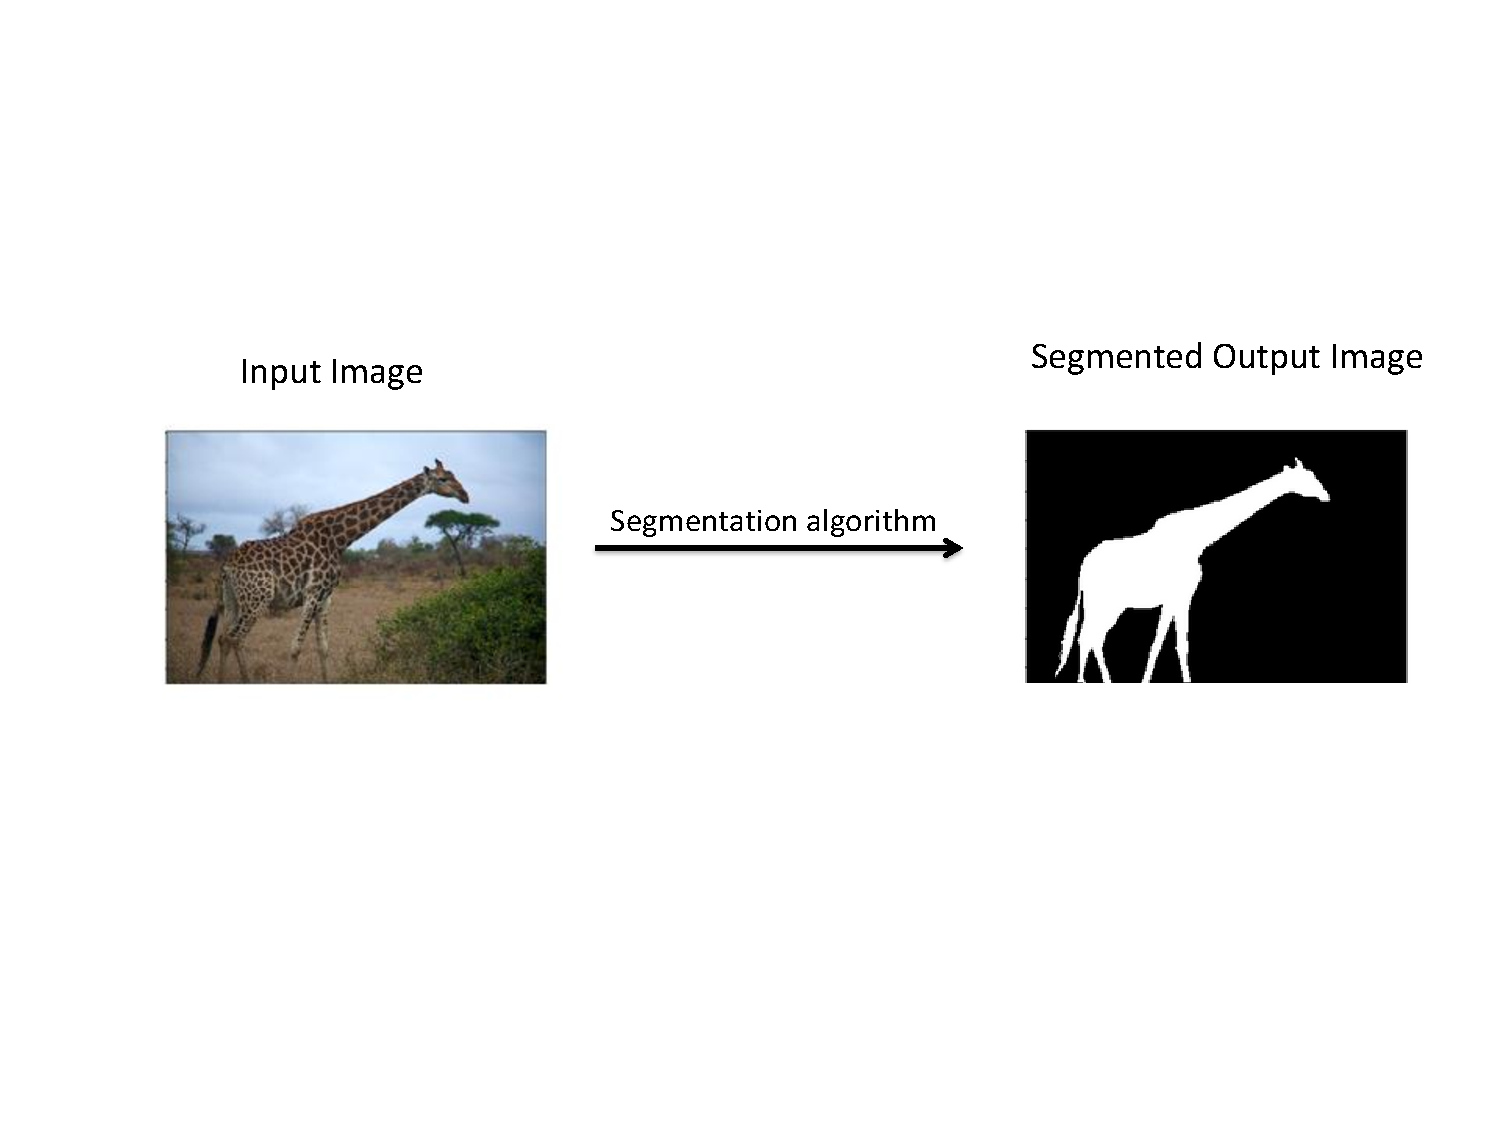
\includegraphics[width=\linewidth]{./Figure/segmentation.pdf}
\caption{Binary Image Segmentation. The task is to group the pixels into foreground (i.e object of interest Giraffe) and the background.}
\label{fig:binary_image_segmenatation}
\end{figure}

There are five major categories of image segmentation: thresholding, edge, clustering, region pixel classification and partial differential equation based segmentation methods.

Thresholding segmentation changes an image into a binary image using a threshold value~\cite{bali2015review,khan2014survey}. Thresholding is sensitive to noise and is unable to detect edges. Region-based segmentation the groups pixels into homogeneous regions , this methods is both computationally and compute (i.e. slow) expensive. Clustering based segmentation groups a similar pixels into clusters, finding the optimal number of cluster is difficult and also it is computationally expensive. Edge-based segmentation, groups pixels based on discontinuities such as texture or intensity in the image, this methods is computationally expensive and finding robust edges is non-trivial~\cite{upadhyay2017survey}. PDE based segmentation methods are considered in this study, due to their sequential nature in performing image segmentation and therefore can be framed into a sequential problem, such that a RNNs based methods may be used to learn the PDE process for performing image segmentation. PDE based segmentation are also computationally expensive.



% Image segmentation techniques can be grouped into five categories: region-based segmentation, clustering based segmentation, pixel classification based segmentation, edge-based segmentation and thresholding based segmentation and partial differential equation based methods. Thresholding segmentation converts an image into a binary image using a threshold~\cite{bali2015review,khan2014survey} . Region-based segmentation the image is divided into subset where the neighbouring pixels with one subset are similar according to a defined criterion. Clustering based segmentation groups a set of pixels in such a way that pixels in the same cluster are more similar to each other than those in another cluster. Edge-based segmentation, the edges refer to the pixels at which there is an abrupt change in intensity or texture and an image is segmented by detecting those discontinuities. The shortcomings of edge segmentation methods are true edges are often fragmented by noise in the image and in most cases leads to misidentification of edges. In this research, we will focus on partial differential equation based segmentation methods. 


Let $I_{0}$ denote an observed image on a 2D open and bounded domain $\Omega$. Segmentation means finding a  visually meaningful edge set $\Gamma$ that leads to a complete partition of $\Omega$. Each Connected Component $\Omega_{i}$ of $\Omega \setminus \Gamma $ should correspond to at most a real physical object. This lead to two consideration to the segmentation problem, firstly is how to formulate a model that appropriately combines the effect  of both edges set $\Gamma$  and it's segmented regions (i.e  $\{ \Omega_{i}, i =1,2...\}$) and secondly finding the representation of the geometry of both the edge set and the regions and also the representation of the segmentation model. In the Variational PDE approach, the two problems are resolved in literature. the Mumford and Salah model was proposed a solution to the first problem and secondly work of Osher and Sethian  on the level set representation is the solution to the second problem~\cite{mumford1989optimal,osher1988fronts}.



\subsection{PDEs image segementation}
\label{sec:partial_differential_equation_segmentation_based_methods}



Over the past two decades, a large number of partial differential equation (PDE)-based approaches have been developed for image segmentation. Among them, Geometric Active Contour Model (GACM) is a famous image segmentation approach~\cite{chen2013fast,zhang2010active,truc2011homogeneity,ali2018segmentation,chan2001active,chen2011noisy}. The existing GACMs are mainly categorized into two types, namely edge-based models and region-based models~\cite{caselles1993geometric,caselles1997geodesic,paragios2001gradient} . 

These two models firstly establish an energy function of the image and then obtain an active contour using variational principle and gradient descent flow technique. The iterative formula is finally derived via difference method. Employing gradient information in level set representation or not is an important difference between the models. Edge-based models utilize the gradient information to control the curve evolution. These models contain an edge-based boundary detector mostly, which is always a positive and decreasing function called Edge-Stopping Function (ESF). When the ESF equals to zero, the evolution curve will stop on the desired boundary of the object.

In reality, these images are mostly digital images, whose discrete gradients are bounded and ESF may never be zero on edges. Hence, the boundary detector fails to find the true contour of the object. The obtained active contour sometimes crosses the true contour edges. Contrasted to edge-based models, region-based GACMs have many advantages. Region based GACMs introduce statistic information inside and outside the contour into a total energy function. Since region-based GACMs exploits  statistical information, they are less sensitive to noise and have better performances for images with weak edges or without edges. On the other hand, unlike edge-based GACMs, region-based GACMs are less sensitive to the location of initial contour. Although region-based GACMs are able to segment many images effectively, they still cannot provide satisfying results for images with intensity in-homogeneity (i.e smooth intensity change inside originally homogeneous regions).  





\subsection{Variational level set}
Variational level set is an implicit implementation of active contour (AC). The main ideas of applying AC for image segmentation is to start with an initial random (guess) contour $\mathbf{C}$ which is represented in a form of closed curves. The curve is then iteratively modified by shrinking or expanding under an image-driven forces until it reach to the boundaries of the desired objects. The entire process is called \textit{contour evolution} or \textit{curve evolution}, denoted as $\frac{\partial \mathbf{C} }{\partial t}$.

There are two main approaches in active contours: snakes and level sets. Snakes explicitly move predefined snake points based on an energy minimization scheme, while level set approaches move contours implicitly as a particular level of a function. Level set (LS)-based or implicit active contour models have provided more flexibility and convenience for the implementation of active contours, thus, they have been used in a variety of image processing and computer vision tasks~\cite{le2019recurrent}.


The basic idea of the implicit active contour is to represent the initial curve $\mathbf{C}$ implicitly within a higher dimensional function, called the
level set function $\phi(x,y):\mathbf{\Omega} \rightarrow \mathbb{R}$, such as $\mathbf{C}=(x,y):\phi(x,y)=0,\forall(x,y)\in \mathbf{\Omega} $, where $\mathbf{\Omega}$ denotes the entire image plane. 


A zero level set function is used to formulate the contour, i.e., the contour evolution is equivalent to the evolution of the level set function, i.e.,  $\frac{\partial \mathbf{C} }{\partial t}  =  \frac{\partial \mathbf{\phi(x,y)} }{\partial t}$. The reason of using the zero level set is that a contour can be defined as the border between a positive area and a negative area. Thus, everything on the zero area belongs to the contour and it is identified by signed distance function as follows:



\[ \phi(x) =  \begin{cases} 
      d(x,\mathbf{C})  \quad  & if\hspace{0.2em}x\hspace{0.2em} is \hspace{0.2em} inside \hspace{0.2em} \mathbf{C}  \\
        0 \quad  & if\hspace{0.2em} x\hspace{0.2em} is\hspace{0.2em} on \hspace{0.2em} \mathbf{C}  \\
      -d(x,\mathbf{C})  \quad   &if\hspace{0.2em} x \hspace{0.2em} is\hspace{0.2em} outside \hspace{0.2em} \mathbf{C} 
  \end{cases}
\]

where $d(x,C)$ denotes the distance from an arbitrary position to the curve. One of the most popular region based active contour models is proposed by Chan-Vese~\cite{chan2001active}.

\subsubsection{Chan-Vese image segmentation}

The Chan-Vese algorithm is a region-based segmentation algorithm which is based on the ideas of contour evolution, the Mumford-Shan functional, and the level set of Osterand Sethian ~\cite{chan2001active,tai2006image,caselles1997geodesic}. This algorithm has several advantages. Since the gradient-based information is replaced  by  a criterion which is related to region homogeneity:
\begin{itemize}
    \item it  can  detect  the  region  contours  with  and  without strong gradient information
    \item it is able to detect interior contours
    \item  the  initial  curve  does  not  necessarily  have  to  start around  the  objects  to  be  detected  and  can  be  placed anywhere in the image instead
    \item it partitions the image into two regions, the detected objects as the foreground and the rest as the background
    \item it does not need to have noise removal preprocessing in advance
\end{itemize}

\begin{figure}[H]
\centering
  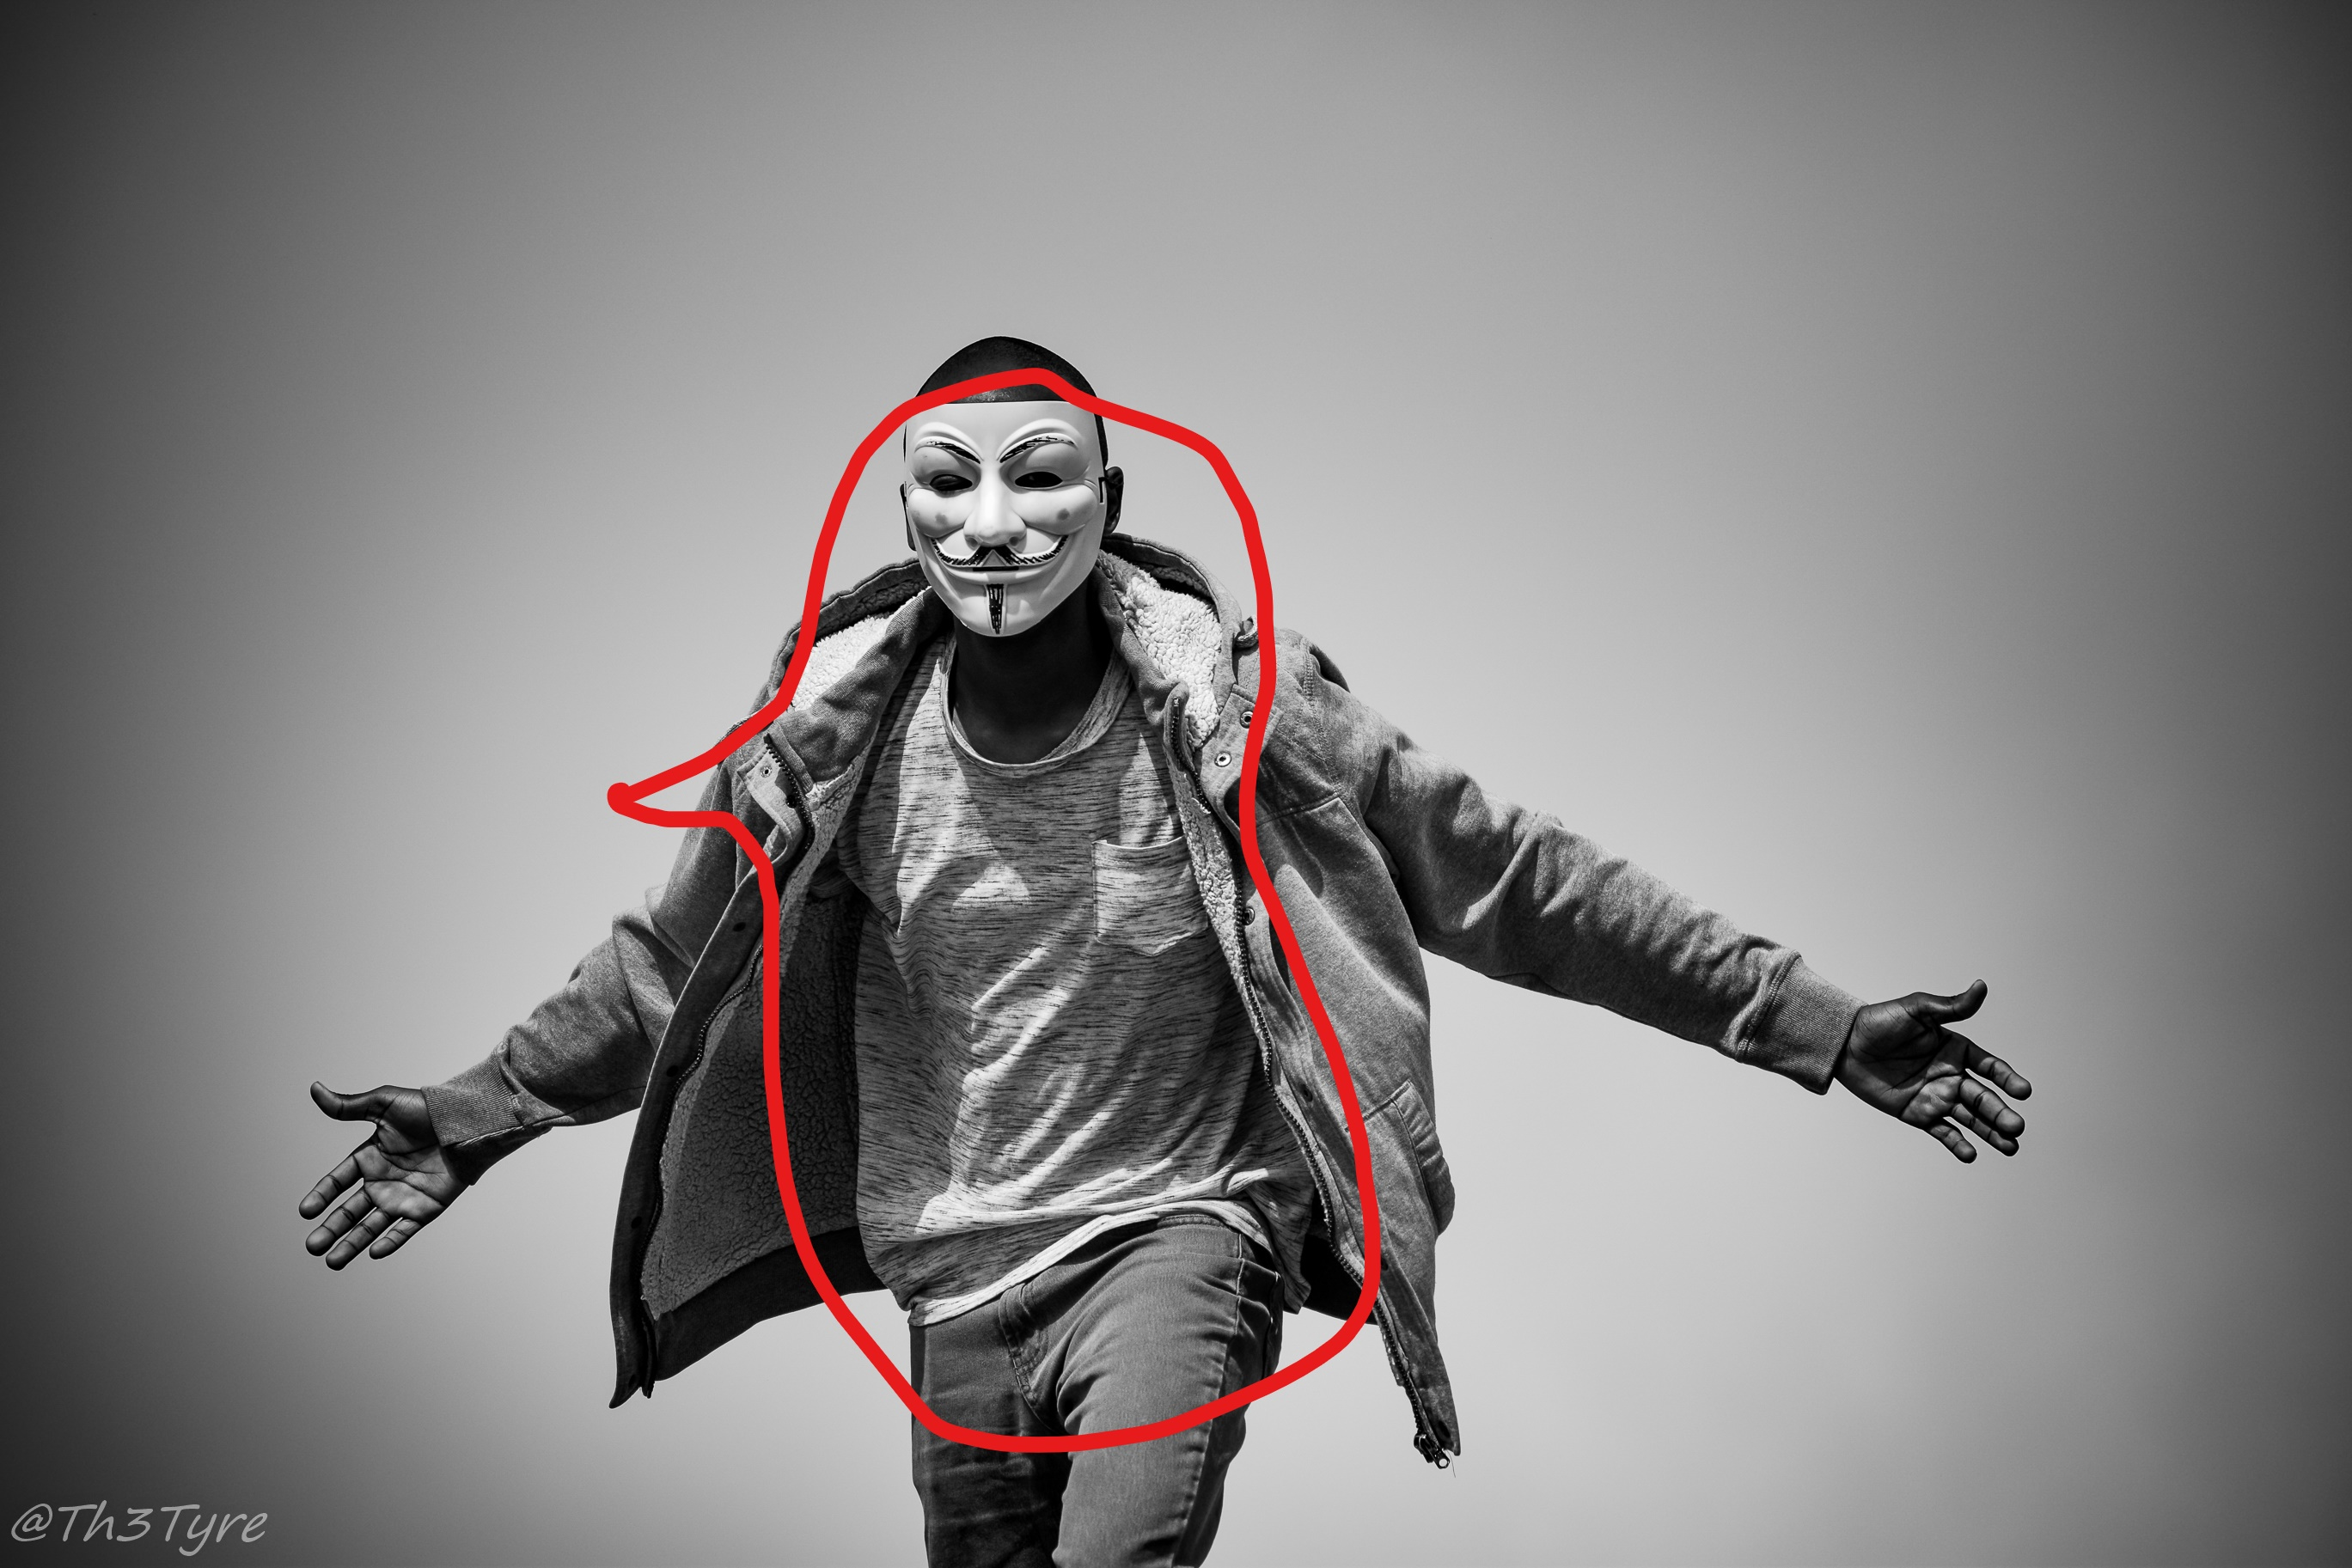
\includegraphics[width=0.5\linewidth]{Figure/me.jpg}
 \caption{The image is defined on $\mathbf{\Omega}$ (the big rectangle), the (arbitrary) red curve is $\mathbf{C}$.}
 \label{fig: cv_image}
\end{figure}





Let $\mathbf{\Omega} \in \mathbb{R}^{2}$ be a bounded open subset and $\mathbf{I}: \mathbf{\Omega} \rightarrow \mathbb{R}$ be a difference image which consist of two homogeneous regions $\mathbf{\Omega}_{1}$ and $\mathbf{\Omega}_{2}$ ($\mathbf{\Omega} = \mathbf{\Omega}_{1} \bigcup \mathbf{\Omega}_{2}$). The Chan-Vese algorithm finds a contour that partitions the difference image into two sub-regions $\mathbf{\Omega}_{1}$ and$\mathbf{\Omega}_{2}$, that describe an optimal piece-wise~\footnote{A piecewise-defined function (also called a piecewise function or a hybrid function) is a function defined by multiple sub-functions, each sub-function applying to a certain interval of the main function's domain, a sub-domain.} constant approximation of the image. The contour $\mathbf{C}$ is determined by minimizing the segmentation energy, ~\cite{chan2001active}

\begin{equation}
    E(\mathbf{C},c_{1},c_{2}) = \lambda_{1} \int_{\mathbf{\Omega}_{1}} (\mathbf{I}(x,y)-c_{1})^{2}dxdy +
    \lambda_{2} \int_{\mathbf{\Omega}_{2}} (\mathbf{I}(x,y)-c_{2})^{2}dxdy + \mu Length(\mathbf{C})
\label{equ:Chan_Vese_equation}
\end{equation}

where $c_{1}$ and $c_{2}$ denote the average intensities in the regions inside $\mathbf{\Omega}_{1}$ and outside $\mathbf{\Omega}_{2}$ $\mathbf{C}$ respectively, and $\lambda_{1}$, $\lambda_{2}$ and $\mu$ are the weighting parameters for the fitting terms and regularization, respectively. If $\mu$ is large, only larger objects are detected, while for small $\mu$,objects of smaller size are also detected.

The Chan-Vese algorithm uses the level sets of Osher and Sethian not arbitrary point to control the contour $\mathbf{C}$~\cite{caselles1997geodesic}.  The contour $\mathbf{C}$ can be represented as a zero level set function  $\phi$ over the domain of  $\mathbf{\Omega}$, which satisfy the following conditions:

\[ \forall (x,y) \in \Omega \begin{cases} 
      \{(x,y):\phi(x,y)  < 0 \} \quad in & \mathbf{\Omega}_{1}  \\
      \{(x,y):\phi(x,y)  = 0\} \quad on & \mathbf{C} \\
      \{(x,y):\phi(x,y)  > 0\} \quad in  & \mathbf{\Omega}_{2}
  \end{cases}
\]



Using the Heaviside function $H$, which is defined by

\[ H(z) = \begin{cases} 
      0 \quad if & z \leq 0  \\
      1 \quad if & z >   0
  \end{cases}
\]

and it distributive derivative $\sigma = \partial H/ \partial z $, Equation~\ref{equ:Chan_Vese_equation} can be written as follows

\begin{equation}
    E(\phi,c_{1},c_{2}) =  \int_{\mathbf{\Omega}} \Big ( \lambda_{1}\mathbf{I}(x,y)-c_{1})^{2}(1 - H(\phi (x,y)) +
    \lambda_{2} (\mathbf{I}(x,y)-c_{2})^{2}  H(\phi (x,y))  \big )dxdy
\label{equ:Levelset_Chan_Vese_equation}
\end{equation}

The energy functional $E(\phi,c_{1},c_{2})$ can be minimized with respect to the constants $c_{1}$ and $c_{2}$ for a fixed $\phi$, according to Osher and Sethian~\cite{caselles1997geodesic}.


\[ \begin{cases} 
      c_{1} = \Gamma(\mathbf{I}) \quad if & \phi \geq 0  \\
      c_{2} = \Gamma(\mathbf{I})   \quad if & \phi <   0
  \end{cases}
\]


where $\Gamma(\mathbf{I})$ computes the average of the pixels intensity values of $\mathbf{I}$ for a given region of interest, Using the gradient descent methods, the Euler-Lagrange equation for $\phi$ can established by minimizing the energy functional $E(\phi,c_{1},c_{2})$ with respect to $\phi$, for fixed $c_{1}$ and $c_{2}$ governed by the mean curvature and error terms~\cite{caselles1993geometric,celik2010multitemporal} defined as,

\begin{equation}
\frac{\partial \phi (x,y)}{\partial t} =  \delta \phi (x,y) [k \phi (x,y)  - \mu - \lambda_{1}(\mathbf{I}(x,y) -c_{1})^{2} + \lambda_{2}(\mathbf{I}(x,y) -c_{2})^{2} ]
\label{equ:levelset_derivative}
\end{equation}

where $\delta$, $k$ is a Dirac delta function and curvature respectively. The curvature $k$ is given by,


\begin{equation}
k(\phi (x,y)) = - div(\frac{\Delta \phi}{|\Delta \phi|}) = - \frac{\phi_{xx} {\phi_{y}}^{2} - 2\phi_{x} \phi_{y} \phi_{xy} + \phi_{yy} {\phi_{x}}^{2} } { ({\phi_{x}}^{2} + {\phi_{y}}^{2})^{1.5}}
\label{equ:curvature}
\end{equation}

where $\partial_{x} \phi_{t}$ and $\partial{xx} \phi_{t}, \partial{yy} \phi_{t}$ are the first and second derivatives of $\phi_{t}$ with respect to x and y directions. Intuitively the curvature $k$ tells us by how much the tanget is changing along the curve. We use $\phi_{t}$ to denote $\phi$ at the $t^{th}$ iteration. Now, intuitively the curve evolution can be represented as time series process, where we redefine the curve updating in a time series form for the LS function $\phi_{t}$ as,


\begin{equation}
\phi_{t+1} = \phi_{t} + \alpha \frac{\partial \phi_{t}}{\partial t}
\label{equ:curve_evolution}
\end{equation}



The LS at time $t+1$ depends on the previous LS at time $t$ and the curve evolution $\frac{\partial \phi_{t}}{\partial t}$ with a learning rate $\alpha$.
% The computation is performed on the same dimension as the image plane $\mathbf{\Omega}$ , therefore, the computational cost of level set methods is high and the convergence speed is quite slow. 


\subsection{Conclusion}
The levelset methods are computationally expensive and also the convergence rate is quite slow, this is due to the computation being performed on the same dimension as the image plane $\mathbf{\Omega}$. Levelset methods are also highly dependent on the initialization of the velocities for propagating the levelset function, if the velocity flow is not constant the levelset function becomes strongly distorted, which mean that its gradient may become very large or very small around the edges~\cite{ovsyannikov2013further}. In our work we demonstrate that the using recurrent models such as the  ESN, LSTM, GRU and RNN we can learn the process of iteratively segmenting an image similar to a levelset function. 



\newpage
\section{Methodology}
\label{sec:Methodology}


\subsection{Introduction}
% \label{sec: Introduction_method}
% \par{This section is divided into two folds, classification which is used as a benchmark for the ESN and segmentation which forms the basis of the this study. The classification problem  considered is the MNIST digit recognition.}
The body of this work is two-fold, \textit{the data generation} and \textit{the image segmentation}. Figure~\ref{fig:research_design}, shows an overview of the research design, the data generations step using a variational levelset (PDE)~\ref{equ:Levelset_Chan_Vese_equation} to generate a sequence of images ${\mathbf{X}}_t$, and the image segmentation step to learn the variational levelset. Learning the variational levelset is formulated as spatio-temporal problem, such that we use convolutional recurrent neural networks (CESN, CRNN, CLSTM and CGRU) and 3D-convolutional neural network and the we  propose a comparative study of these models.

% This research is divided into two main parts: \textit{the data generation step} and \textit{the image segmentation step}. Figure~\ref{fig:research_design} shows an overview of the experimental setup. The data generation step involves using the variational levelset defined in Equation~\ref{equ:Levelset_Chan_Vese_equation} to generate a sequence of segmented images.

% The second phase of this research is called the \textit{the image segmentation step}. In this step we will use the ESN to learn to segment the PDE generated images. Lastly, a comparison study between the ESN and RNN (LSTM) is done so that the optimal segmentation technique will be declared along with the selected optimization parameters.

% \subsection{Image Segmentation}
% \label{sec:image_segemenation}
% \subsection{Benchmark approach}
% \label{sec:benchmark_approach}


% \par{The MNIST database is commonly used to evaluate performance of many machine learning methods in theri ability to recognize handwritten digits. The dataset consist of $60000$, $1000$ images in the training and testing set respectively, with the corresponding labels ranging from $0$ to $9$.  Most classification machine learning models are evaluated on their error rate (i.e.  minimization of the loss function) and the best score on MNIST, an error rate of $\mathbf{0.21\%}$, currently held by a committee of 5 neural networks~\cite{wan2013regularization}. Eaach network consist of two convulational layers with $32-64$ feature maps in each respectivley, followed by a fully connected layer of $150$ rectifier linear unit sparsely connected thanks to DropConnect, and a final softmax classification layer.
% }


% \par{In this section, we first present the method used to classify images with an ESN, and then we describe the transformations applied  to  images  to  improve  the  performances. }


% \subsubsection{Transformation from spatial domain to temporal signal}
% \label{sec:from_image_to_temporal_signal}


% \par{The MNIST handwritten digit classification task consist of 28$\times$28 images black and white images, each containing a digit $0$  to $9$ (10 labels). In order to represent the images as time series, each image is considered as a matrix  $I_{n} \in \mathbb{R}^{d_{i} \times d_{i}}$, where $n$ denotes image index and $d_{i}=28$ is the image dimension, with scaled pixel values to $[0,1]$. The corresponding label $y_{n}$ is a integer between $0$ and $9$ according to the digit represented by $I_{n}$.}

% \par{The problem is then to classify each matrix $I_{n}$ in the class $y_{n}$ corresponding to the digit that represent it. Then this becomes a classification problem where the classifier  $c:I_{n}\rightarrow y_{n}$, where $y_{n}\in \{0...9\}$, as to establish to which class the matrix $I_{n}$ belongs to. The evaluation of the classifiers performance, is expressed as the percentage of the matrix classified in the wrong class $E(y,\hat{y})\in [0,100]$, on the training and testing set.}

% \par{In order to feed in the matrix $I_{n}$ into the reservoir, the matrix is transformed into a temporal signal, by treating the matrix as a sequence of rows and columns. This is because the structure along the columns is different to the rows, thus we want to capture temporal sequences. This is achieved, by transforming the spatial dimensions to temporal sequence.}







% \par{ As we consider a processing column-wise (horizontal scanning), we have $N_{u}=N_{i}$ reservoir and inputs and for each input $(u_{i})_{t} = (I_{n})_{ij}$, where $t=n \times N_{i}  + j$. Hence, the i-th reservoir input takes, as time step $t$, the value of the (i,j) element of the $n-th$ matrix with both $n$ and $j$ defined according to $t$. Then, as a result we get $N_{i}$ time series composed of all images put side by side. For each time step $t$ which is a multiple of $N_{i}$ a new image is introduced, the idea behind this method is to put one dimension of the images in the memory of the reservoir so that it can create a set of features of the current image and use these feature to classify the image. Thus, the reservoir must have enough memory to store a full image.
% }

\subsection{Research Aims And Objectives}
\label{sec:research_aims_and_objectives}
This research aims to:
\begin{itemize}
    \item formulate variational levelset as spatio-temporal problem, and
    \item learn the variational levelset image segmentation process using deep learning methods, thereby 
    \item realizing a computational cheap image segmentation refinement method to variational levelset, and 
    \item understand the setting of the reservoirs essential parameters in achieving state of the art results for a given task. 
\end{itemize}

The above aims of this research will be achieved through the following objectives :
\begin{itemize}
    \item generating a sequence of image using the variational levelset method, this serves as a spatio-temporal dataset for solving the problem.
    \item compare the performance of the ESN to RNN, LSTM, GRU and CNN in learning the spatio-temporal variational levelset process.
    \item determine the relationship of the leaking rate, reservoir size to the performance. 
\end{itemize}


\subsection{Research Hypothesis}
\label{sec:research_hypothesis}
The hypothesis of this research is:
\begin{itemize}
    \item the ESN is able to learn the solve the iterative approach for segmenting an image, thereby learning the first order variational levelset for binary image segmentation.
    \item due to the optimization of the many parameters of CESN  as compared to other models, it will prove difficult to establish the echo state property such that we get optimal performance.
\end{itemize}




\subsection{Research Questions}
\label{sec:research_questions}
Here we present our research questions that will guide us through the research process. The questions we are aiming to answer are:
\begin{itemize}
    \item how to generate a sequence (i.e. spatio-temporal) data $X_{t}$ from a single image $\mathbf{I}$ if we consider $\phi_{t}$ in the variational levelset  as the reservoir in CESNs with the same updating manner?
    \item can we learn variational levelset (PDE) using CESN? 
    \item can we find a set optimal parameters of the CESN to achieve optimal performance in learning variational levelset (PDE)? 
    \item can the CESN outperform the  variational levelset (PDE), in cases where the  variational levelset solution is not optimal?
\end{itemize}

\subsection{Data Acquisition}
\label{sec:Datasets}
For this work, the Weizmann Segmentation (WSD)~\cite{AlpertGBB07} , Berkeley Segmentation Data Set and Benchmarks (BSD)~\cite{amfm_pami2011}, CIFAR-10 and CIFAR-100~\cite{krizhevsky2009learning} datasets for training, validation and testing of models. The CIFAR-10 consist of 60000 \textit{32 $\times$ 32} RGB images in 10 classes, with 6000 images per class. The CIFAR-100 is similar to the CIFAR-10 dataset except it has 100 classes containing 600 images each.  WSD database consist of 200 \textit{300 $\times$ 200} RGB images that clearly depict one or two object/s in the foreground that differ from its surroundings by either intensity, texture, or other low level cues.  BSD consist of \textit{481 $\times$ 321} , 200, 100 images for training and testing set, respectively. These dataset consist of natural images.

% \par{
% % The Berkeley Segmentation Data Set and Benchmarks 500 (BSR)~\cite{amfm_pami2011} and 
% % the  Massachusetts Roads dataset~\cite{mnih2013machine} were used in this experiment. The BSR dataset consists of all of the grayscale and color segmentations for 300 images. The images are divided into a training set of 200 images, and a test set of 100 images. Each image has a resolution of 184x231. Massachusetts Roads dataset consist of  of 1171 image-mask  pairs  and  are  separated  into  1108  training  images,  14 validation  images  and  49  test  images.  Each  image  has  a resolution of 1500x1500 with a scale of 1 m2/px.
% In this experiment we used 4 different database. The CIFAR-10 and CIFAR-100 datasets are used in this experiment. The CIFAR-10 consist of 60000 \textit{32 $\times$ 32} RGB images in 10 classes, with 6000 images per class. The CIFAR-100 is similair to the CIFAR-10 dataset except it has 100 classes containing 600 images each~\cite{krizhevsky2009learning}. The Weizmann segmentation database consist of 200 \textit{300 $\times$ 200} RGB images that clearly depict one or two object/s in the foreground that differ from its surroundings by either intensity, texture, or other low level cues~\cite{AlpertGBB07}. The Berkeley Segmentation Data Set and Benchmarks 500 (BSD)~\cite{amfm_pami2011} consist of \textit{481 $\times$ 32} , 200, 100 images for training and testing set, respectively. These dataset consist of natural images. 
% }



\subsection{Model Evaluation}
\label{sec:model_evaluation_and_optimization}
 In order to have a guided analysis for the segmentation task, the following metrics are defined in the context of the task. Consider a segmentation task such that the positive class is the foreground pixels (1's) and the negative class is the background pixels (0's). The following metrics are defined as follows:



\subsubsection{Confusion Matrices}
Consider the following confusion matrix between the predicted and the actual classified pixels. It describe the performance of a model on the validation and testing datasets, where the actual true pixels are given. Figure~\ref{fig:confusion_matrix} shows a  generic confusion matrix diagram such that:
%  A confusion matrix, is a tool for visualization between the predicted pixels class and the actually classified pixels. It describes the performance of a model on the testing set where the actual true values are known. Figure~\ref{fig:confusion_matrix} shows a general confusion matrix diagram such that:
\begin{table}[H]
\centering
    \begin{tabularx}{\textwidth}{c|c|c|c|c} 
        \multicolumn{2}{c}{}&\multicolumn{2}{c}{Predicted}&\\
        \cline{3-4}
        \multicolumn{2}{c|}{}& \small Negative: Background pixels & \small Positive: Foreground pixels & \multicolumn{1}{c}{Total}\\
        \cline{2-4}
        \multirow{2}{*}{Actual}& \small Negative: Background pixels & $a$ & $b$ & $a+b$\\
        \cline{2-4}
        & \small Positive: Foreground pixels & $c$ & $d$ & $c+d$\\
        \cline{2-4}
        \multicolumn{1}{c}{} & \multicolumn{1}{c}{Total} & \multicolumn{1}{c}{$a+c$} & \multicolumn{    1}{c}{$b+d$} & \multicolumn{1}{c}{$N$}\\
    \end{tabularx}
    \caption{Confusion matrix.}
    \label{fig:confusion_matrix}%
\end{table}


\begin{itemize}
    \item a is the number of correct predictions of a foreground pixel called true positive (TP).
    \item b is the number of incorrect prediction of a foreground pixel called false positive (FP).
    \item c is the number of incorrect prediction of a background pixel called false positive (FN).
    \item d is the number of correct predictions of a background pixel called true positive (TP)
\end{itemize}


\subsubsection{Precision}
% Precision is the proportion of the predicted foreground pixels that were correct. Precision (P) is calculated as follows,
Precision is the proportion of predicted foreground pixels in the iterative segmentation results that match with the ground-truth. Precision (P) is calculated as follows,

% Precision is the proportion of the predicted positive pixels that were correct. Precision (P) is calculated as follows,
\begin{equation}
    P = \frac{\textit{\text{correctly Predicted Foreground Pixels}}}{\textit{\text{total number of Predicted Foreground Pixels}}} = \frac{d}{b+d} 
     \label{equ:precision}
\end{equation}

The precision is a function of FP, which means it measures the rate of falsely predicting foreground pixels as background, and therefore segmentation performance is sensitive to over-segmentation. The over-segmentation results in low precision scores.

\subsubsection{Recall}
Recall is the proportion of ground-truth foreground pixels in the iterative segmentation results that were correctly identified. Recall (R) is calculated as follows,

% Recall can be defined as the proportion of positive pixels that were correctly identified. Recall (R) is calculated as follows, 
\begin{equation}
    R =  \frac{\textit{\text{correctly Predicted Foreground Pixels}}}{\textit{\text{total number of Actual Foreground Pixels}}} = \frac{d}{c+d}
    \label{equ:recall}
\end{equation}

The recall is a function of FN, which means it measures the rate of falsely predicting background pixels as foreground, and therefore the segmentation performance is sensitive to under-segmentation. The under-segmentation results in low recall scores.

\subsubsection{ F1 Score}
The trade-off between precision and recall is summarised using the $F_{1}Score$
which is a value that can be described as the harmonic mean of precision and recall, it is calculated as follows, 
\begin{equation}
    F_{1}Score = 2*\frac{P*R}{P+R} = \frac{2a}{2a + b + c }
     \label{equ:f1}
\end{equation}

The $F_{1}Score$ takes FP and FN into account and it always between precision and recall, and is useful for contour or boundary matching between predicted segmentation and ground truth segmentation

\subsubsection{Intersection Over Union (IoU)}

The IoU score is a commonly used metric for image segmentation problems. The IoU measure the similarity between ground-truth and predicted regions, between a set of images and it is defined by following equation~\cite{rahman2016optimizing}, 

\begin{equation}
    IoU = \frac{a}{a+b+c}
     \label{equ:iou}
\end{equation}

\subsubsection{Conclusion}

Normally the ability of a model to solve a task is positively correlated to the score of the metric. The metrics used to evaluate the final results on the validation and testing data are the precision, recall, $F_{1} Score$ and IoU. The recall and precision are used to measure the robustness of the models in dealing with the high class imbalance in the dataset, that is in our problem low precision score results in over-segmentation, and low recall results in under-segmentation.

The overall quality of the boundaries or contours segmentation is measured using IoU and the trade-off between over-segmentation and under-segmentation is measure using $F_{1} Score$. The difference between IoU and $F_{1} Score$ as evident from Equation~\ref{equ:iou} is that IoU will penalize incorrect classified results more than $F_{1} Score$, they metrics can be monotonic to one another or positively correlated.


\newpage

\subsection{Formulating the Levelset as a ESN}
\label{sec:reformulating_generation}
In this section, we look at the LS introduced in~\cite{chan2000active} to demonstrate how to formulate the LS as an end-to-end learnable neural network framework under CNNs, RNNs, LSTMs, GRUs and ESNs. Consider training procedure shown in Figure~\ref{fig:research_design}:

\begin{figure}[H]
\centering
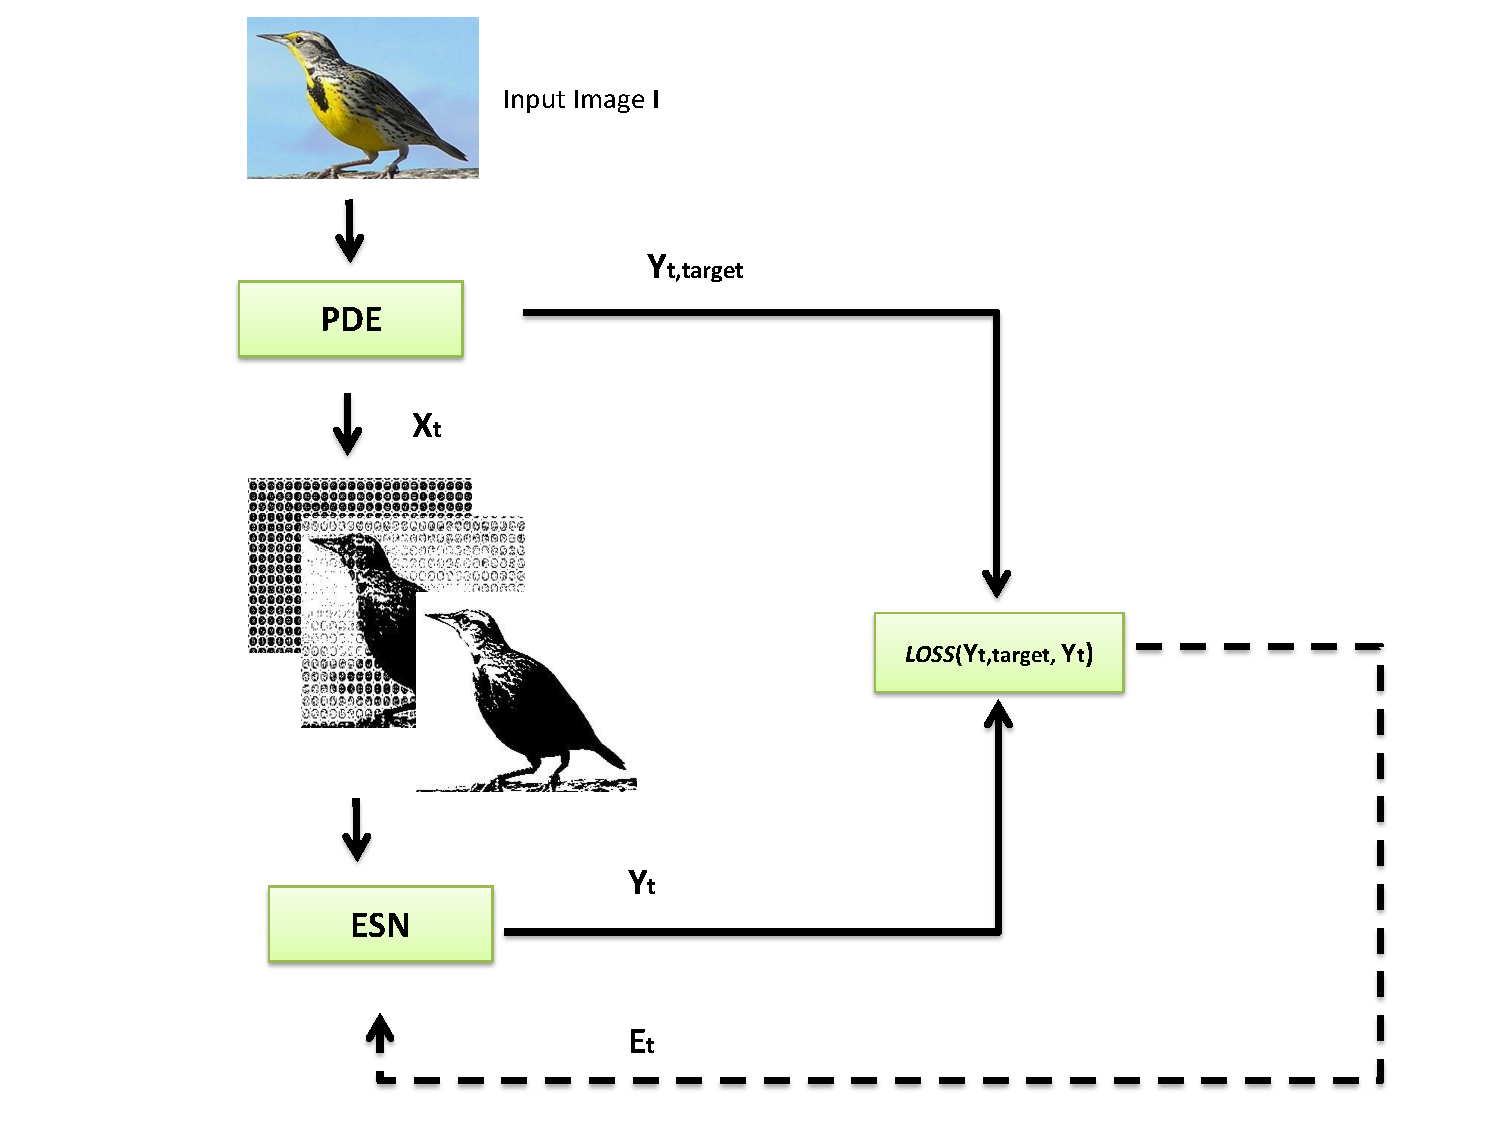
\includegraphics[width=1\textwidth]{Figure/ESN.pdf}
\caption{Iterative segmentation architecture.}
\label{fig:research_design}
\end{figure}

\begin{itemize}
    \item A single input image $\mathbf{I}$ is passed into the LS (e.g., PDE as shown in the ~\ref{fig:research_design}), and the PDE generates a sequence of segmented images (i.e. spatio-temporal dataset) $\mathbf{X}_{t}$ of length $t$ steps.
    \item The LS generated images $\mathbf{X}_{t}$ acts as the ground truth samples $\mathbf{Y}_{t,target}$ 
    to be learned by the model (i.e. CNN, RNN, LSTM, GRU and ESN).
    % \item Input image $\mathbf{I}$ is passed into the LS (e.g., PDE as shown in the ~\ref{fig:research_design}) and the PDE generates a sequence of segmented images  $\mathbf{X}_{t}$ of length $t$.
    % \item The LS generated images $\mathbf{X}_{t}$ are ground truth samples $\mathbf{Y}_{t,target}$ for the model (i.e. CNN, RNN, LSTM, GRU and ESN).
    \item The segmentation process is learned by minimizing the binary-cross entropy loss function (e.g., error) ~$Loss(\mathbf{Y}_{t, target}, \mathbf{Y}_{t})$ through stochastic gradient descent method with momentum, where $\mathbf{Y}_{t}$ is the predictions.
    \item The error/loss $\mathbf{E}_{t}$ is used to adjust the learnrable parameters (e.g., weights) of the CNN, RNN, LSTM, GRU and ESN.
\end{itemize}


\subsubsection{Model Architecture}
The problem we formulated as a spatio-temporal task, therefore we use two types of architecture specialized to capture the spatio and temporal dependencies, a 3D-convolutional neural network (3DCNN)~\cite{tran2015learning, ji20123d, karpathy2014large} and a convolutional recurrent neural network (RCNN)~\cite{ji20123d, wang2016cnn}. 

The 3DCNN architecture consist of 2 3D-convolutional block (Conv3D
$\rightarrow$
BatchNorm3D
$\rightarrow$
ReLU
$\rightarrow$
MaxPool3D
$\rightarrow
$Dropout3D), followed by a 4096-units fully-connected layers and a 4096-units output layer, as shown in Figure~\ref{fig:3dCNN}.  The inputs is a t$\times$64$\times$64, where t is the number of time steps. Both 3D-conv consist of 32 filters each with a kernel 3$\times$7$\times$7, stride 2$\times$2$\times$2, padding 0$\times$0$\times$0 and dilation rate 2$\times$2$\times$2. The conv1 and conv2 inputs channels are 2 and 32, respectively.



\begin{figure}[H]
\centering
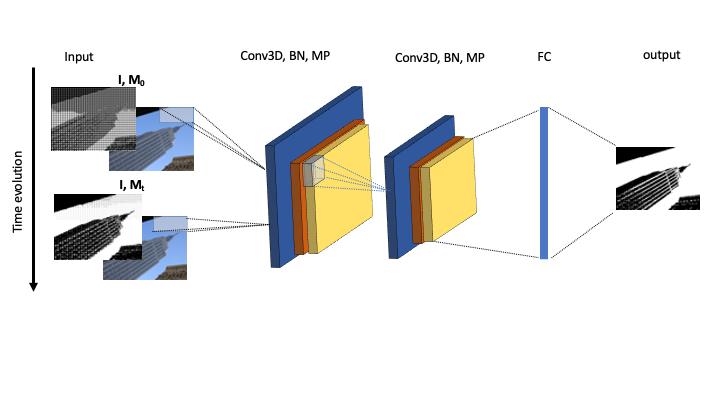
\includegraphics[width=1\textwidth]{Figure/3dcnn.png}
\caption{3D-CNN architecture.}
\label{fig:3dCNN}
\end{figure}


The RCNN architecture consist of 4 2D-convolutional block (Conv2D
$\rightarrow$
BatchNorm
$\rightarrow$
ReLU
$\rightarrow$
Dropout
$\rightarrow$
Conv2D
$\rightarrow$
MaxPool), a RNN layer with 512 ESN/GRU/LSTM units, followed by a fully-connected layer with 4096 units, and a 4096-units output layer, as shown in Figure~\ref{fig:ConvESN}. The inputs is a t$\times$64$\times$64, where t is the number of time steps. The first 2D-conv block consist of 2 inputs channels  32 filters each with a kernel 7$\times$7, stride 2$\times$2, padding 0$\times$0 and dilation rate 2$\times$2.  The second 2D-conv block consist of 64 inputs channels  64 filters each with a kernel 1$\times$1, stride 1$\times$1 , padding 0$\times$0 and dilation rate 1$\times$1, The third 2D-conv block consist of 64 inputs channels  128 filters each with a kernel 7$\times$7, stride 2$\times$2 , padding 0$\times$0 and dilation rate 1$\times$1. The fourth 2D-conv block consist of 128 inputs channels  128 filters each with a kernel 1$\times$1, stride 1$\times$1 , padding 0$\times$0 and dilation rate 1$\times$1.

\begin{figure}[H]
\centering
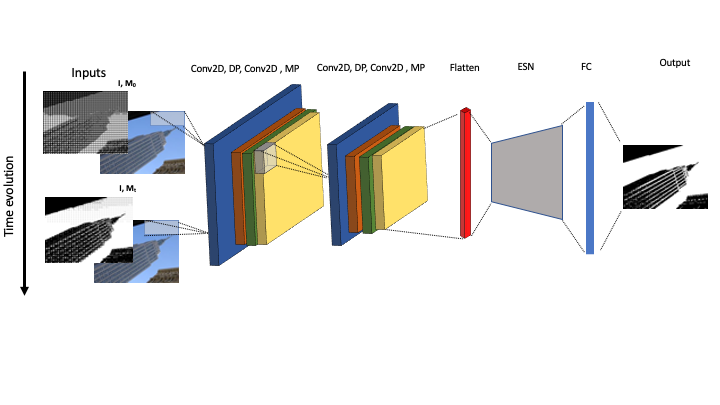
\includegraphics[width=1\textwidth]{Figure/CNN_LSTM.png}
\caption{RCNN architecture.}
\label{fig:ConvESN}
\end{figure}

\subsubsection{Data Generation}
\label{sec:data_generation}

In order to formulate the levelset as an RNN, we need to answer one of our research question, that is how to generate a sequence $X_{t}$ of segmented images from a single image $\mathbf{I}$ using a variational levelset (PDE) as shown in Figure~\ref{fig:research_design}.

\begin{figure}[H]
\centering
  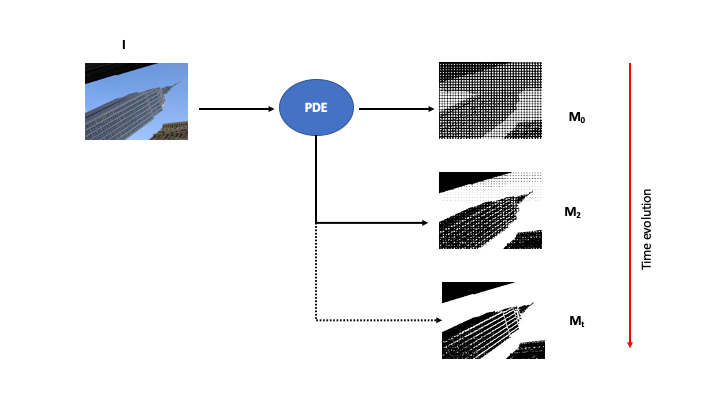
\includegraphics[width=1\textwidth]{Figure/Results/PDE.png}
 \caption{LS Generated training dataset. An input image $\mathbf{I}$ and initial binary mask $\mathbf{M}_{0}$, are feed into the PDE, and at each time step $t$ a corresponding binary mask $\mathbf{M}_{t}$ is generated, where $t$ is the number of iterations to the final optimal segmentation.}
 \label{fig:sample_generated_data}
\end{figure}

The first row is the input image $\mathbf{I}$, the second row is the segmented LS generated a sequence images $X_{t}$.

Consider a grayscale 2D input image $\mathbf{I}$ and an initial binary mask $\mathbf{M}_{0}$. The binary mask  $\mathbf{M}_{0}$ is used to initialize the LS function $\phi_{0}$ such that the outer boundary approximate the object of interest in image $\mathbf{I}$ to be segmented. $\mathbf{M}_{0}$ is defined as a checkerboard with the same dimension as the input image $\mathbf{I}$, as shown in Figure~\ref{fig:sample_generated_data}. The initial binary mask $\mathbf{M}_{0}$ is created using a binary step function, because it is easier to generate new contours and faster for to compute the gradients as compared to a as signed distance map.

The inner $\mathbf{\Omega}_{1}$ and $\mathbf{\Omega}_{2}$  pixels, are computed as $\mathbf{\Omega}_{1}$ being composed of $\mathbf{\Omega}_{1}=\mathbf{M}$, and $\mathbf{\Omega}_{2}$  as the set $\mathbf{\Omega}_{2}=\mathbf{\Omega} \setminus  \mathbf{M}$. $\mathbf{\Omega}_{1}$ is assumed to be a connected component~\cite{garrido2015image}. The evolution of the curve is based on the gradient is based on the homogeneity and heterogeneity of the pixels for to detect continuous objects and edges on the image space, this is done by optimization of gradient descent to minimize the energy of the curve, such that $\mathbf{\Omega}_{1}$ and $\mathbf{\Omega}_{2}$ are computed for each step of the gradient descent, as mentioned in Section~\ref{sec:partial_differential_equation_segmentation_based_methods}




% The LS function $\phi$ is initialized  as a binary step function which takes 1 inside a region and 0 outside. The advantage of using binary step functions as the initial level set functions is that new contours can emerge easily and the curve evolution is significantly faster than the evolution from initial functions as signed distance maps. The levelset (i.e. PDE) takes two inputs \mathbf{I}, the input image $\mathbf{I}$ and an contours mask. The contours is initialized in the 2-D grid as a cheakerbaord with the same dimensions as the input image, which is then treated as an initial LS function  $\phi_{0}$ and it is updated using Equation~\ref{equ:curve_evolution}. The input image is converted into a greyscale image with one color channel. The levelset function $\phi$.........




In this experiment, the LS parameters are initialized as follows: $\lambda_{1}=\lambda_{2}=1$, a 2D convolution with a 3$\times$3 kernel, stride of $\Delta x=\Delta y=1$  is used to compute the gradients and  $\Delta t =0.5$ 
as them time step used for the gradient descent optimization of the energy functional.  The weights of the length term $\mu =0.2$. The number of iteration is 100, which means for each input image we generated 100 segmentation images~\cite{akal2019learning}. These generated images form an iterative sequence for image segmentation using the LS. The implementation of the levelset is adapted from~\cite{chan2000active, vese2002multiphase} and it is implemented in MATLAB~\cite{MATLAB2010}. 
Figure~\ref{fig:sample_generated_data} shows the sample LS generated dataset that is used to learn the LS. As shown in the figure the segmentation has the same dimension as the input image, and it is initialized as a cheakerbox at iteration $X_{0}$. The evolution of the PDE evolved the curve to regions of uniform gradient.

% \newpage

\subsubsection{Data Representation}
\label{sec:data_representation}

The input to the models is a 2-channel image. The first channel is a grayscale input image $\mathbf{I}$, and the second channel is the segmentation mask $\mathbf{M_{t}}$, as shown in Figure~\ref{fig:input_image_reprentation}. Both the input and target images are resized to 64 $\times$ 64. The classes are raw grayscale pixel values.
the input images are passed into the model as 2D vector of  64 $\times$ 64 $\times$ 2 pixels, which then are mapped to target pixels of 64 $\times$ 64. Convolutions are used to reduce and summarize the input vector.


\begin{figure}[H]
\centering
  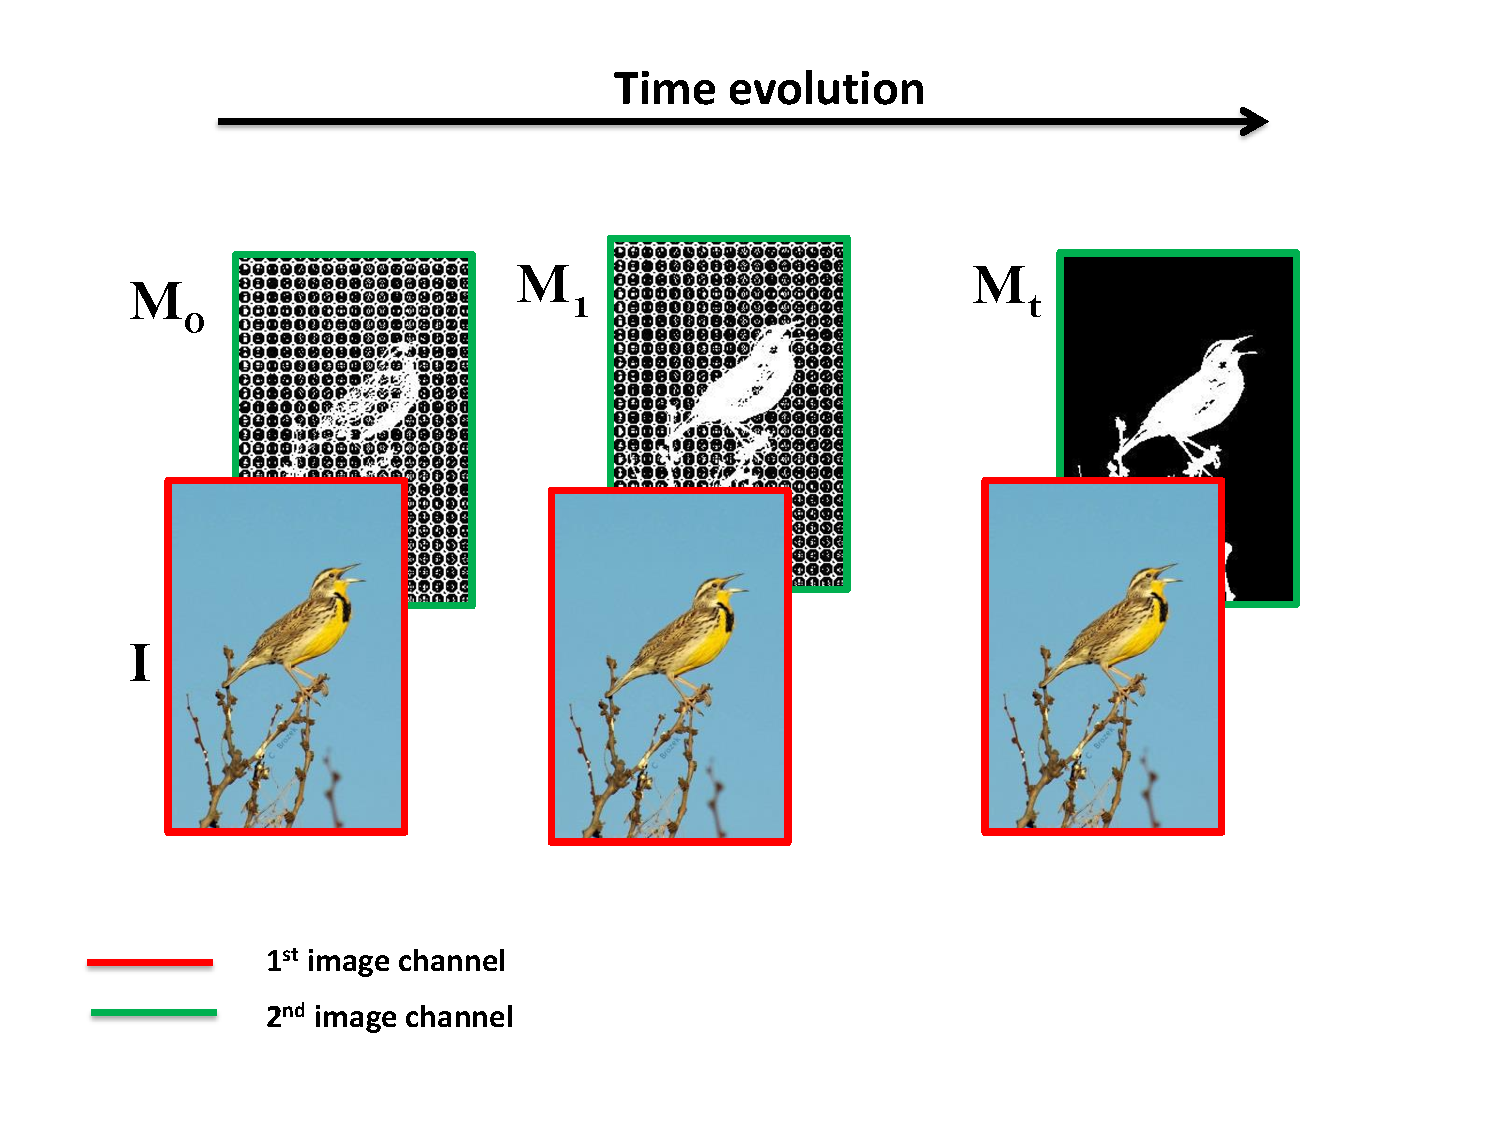
\includegraphics[width=1\textwidth]{Figure/esn_input.pdf}
 \caption{Input image representation.}
 \label{fig:input_image_reprentation}
\end{figure}


\subsection{Training And Inference}
\label{sec:training_and_inference}

Given the a series input ${\mathbf{x}_{0}, ...\mathbf{x}_{t}}$ and target series ${\mathbf{y}_{0}, ...\mathbf{y}_{t}}$ with $t=100$ steps (i.e. samples), we treat the LS evolution as a spatio-temporal problem such that we predict $t+n$ steps into the future, where $n=1$. 

During training the input sequence is ${\mathbf{x}_{0}, ...\mathbf{x}_{t}}$ and the task is predict ${\mathbf{y}_{t+n}}$, the model has to see the entire input history of length n steps, while during inference the output from ${\mathbf{y}_{t-1}}$ is used as input in step ${\mathbf{y}_{t}}$ and it  concatenated with input images as shown
Figure~\ref{fig:input_image_reprentation}. The total number of time steps used is $t=80$ and future steps $n=1$. 


\subsubsection{Loss Function And Optimization}
\label{sec:loss_function}

The binary-cross entropy was is used a loss function, defined as follows,
\begin{equation}
    L = \sum_{i=1}^{2} [Y_{i,target} log(Y_{i}) + (1 - Y_{i,target}) log(1 - Y_{i})],
\end{equation}


where $Y_{i,target}$ and $Y_{i}$ represent the ground truth and predicted class $i$. Intuitively the cross entropy measures the amount of information (i.e.bits) required to represent a given pixel (i.e. background or foreground) from a probability distribution $Y_{i,target}$  as that of probability distribution $Y_{i}$.  And thus a higher cross entropy value result in a model that is unable to distinguish between the background and foreground pixels, in contrast to a lower cross entropy value.

In order to ensure that the models learns, we need minimize the loss function and stochastic gradient descent with momentum is used as the optimization functions as discussed in Section~\ref{sec:Learning}. 
%In order to have a more robust model with generalization we performed several data augmentation such as horizontal and vertical flipping on the input and target image to both the input and target image. All these step were performed randomly in order to reduce bias in the model.  

\subsection{Learning}

\subsubsection{Optimization}
\label{sec:Optimization}
In order to apply the previously mentioned techniques, we use parallel hyperparameter search optimization to choose the optimal leaking rate, sparsity, spectral radius and input scaling for the CESN. The number of hidden (reservoir) units is 4096 neurons. We use Stochastic Gradient Descent (SGD) to optimize our models across a computing cluster. We use mini-batches of 32 examples, momentum of 0.9 and weight decay of 0.1. 

All the models are initialized with learning rates of 0.1 this value is further reduced for $\frac{N_{epoch}}{5}$ step during training, where $N_{epoch}$ is the number of epochs. Parallel runs for each parameter search, are  monitored using tensorboard and the optimal paramaters are selected based on the the minimization of the validation loss and maximization of the IoU, for each of the databases used presented in Tables~\ref{table:cifar_10_hyperparameter},~\ref{table:cifar_100_hyperparameter},~\ref{table:BSD_hyperparameter} and~\ref{table:Weizmann_hyperparameter}.

\subsubsection{Data Augmentation And Preprocessing}
\label{sec:data_augmentation_and_preprocessing}

The total number of generated LS examples for each database WSD, BSD, CIFAR-10 and CIFAR-100 is 200 000, 500 000, 50 000 000 and 60 000 000, respectively. However due to the computational resources constrained in terms of computing time, the CIFAR-10 and CIFAR-100 dataset were limited to 10 000 000. Each database was randomly split into the training, validation and testing set of 80\%, 10\% and 10\%, respectively. 
In order to reduce the effect of overfitting we applied data augmentation. Before presenting an example to a model, we preprocess all the images by resizing them to 64$\times$64 pixels, randomly flipping the images horizontally, vertically with probability 50\%, adding Gaussian noise with a variance of 0.01 and randomly rotating the images for different angles $a \in \{60^{\circ}, 90^{\circ}, 180^{\circ}, 270^{\circ}, 360^{\circ} \}$. 

And lastly the input the pixels of the images $\mathbf{I}$ as shown in Figure~\ref{fig:input_image_reprentation} are normalized between 
[-1, 1], as follows, 

\begin{equation}
    x = \frac{x - X_{mean}}{X_{std}}
     \label{equ:normalization}
\end{equation}

where, x, $X_{mean}$  and $X_{std}$ is the input image, mean and standard deviation images of the entire training set. A total number of 500 epochs is used, with early stopping, to prevent overfitting.

\newpage

\section{Results And Discussion }
\label{sec:Experiments}

\subsection{Introduction}

In this chapter the results of the experiments conducted for this dissertation will be presented. The features of these results will be discussed and important trends and anomalies will be brought to the reader's attention. We present a comparative study for learning the temporal and spatial evolution of the LS iterative image segmentation process as described in Section~\ref{sec:image_segmentation}, several statistical model are compared, namely,the CRNN, CLSTM, CGRU and 3DCNN all versus CESN, and also a detailed analysis of the CESN is also considered. The experiments are conducted using small databases, WSN and BSD, and larger databases CIFAR-100 and CIFAR-10.


\subsection{Weizmann}
\label{sec:Weizmann}

\subsubsection{Introduction}

In this experiment we consider a WSD database, where there is a clear distinction between the foreground and background, the images consist of one or two objects. The database consist of 200 images in total and thus is the smallest database in our experiments.

\subsubsection{Results And Discussion}

Table~\ref{table:Weizmann_hyperparameter} shows the optimal parameters for each model selected based on the performance of the models~\footnote{CESN, CRNN, CLSTM, CGRU and 3DCNN are all referred as \textbf{models} for brevity.} on the validation set. The input images are resized to 64$\times$64, therefore, the number of fully-connected units in and hidden units for the CESN, CRNN, CLSTM, CGRU and 3DCNN is 4096, and the optimal leaking rate, spectral radius, sparsity and input scaling for CESN are 0.0173, 0.9, 0.8 and 1, respectively. The optimal parameters are chosen by maximizing the IoU on the validation set.

\begin{table}[H]
    \centering
    \caption{WSD dataset optimal parameters for the CESN, CRNN, CLSTM, CGRU and 3DCNN}
    \resizebox{\linewidth}{!}{
    \begin{tabular}{ccccccc}
    \hline
    \textbf{Model}  & \textbf{Hidden size} & \textbf{Leaking rate} & \textbf{Sparsity} & \textbf{Spectral radius} & \textbf{Input scaling}\\
    \hline
      CESN    & 4096  & 0.0713 &  0.8 &  0.9  &  1 \\
      CRNN    & 4096 & -  &  -  &  -   & -     \\
      CLSTM   & 4096  &    &  -  &  -   & -      \\
      CGRU   &  4096  & -  &  -  &  -   & -       \\
      3DCNN   & 4096  & -  &  -  &  -   & -       \\
    \hline
    \end{tabular}}
    \label{table:Weizmann_hyperparameter}
\end{table}

Figure~\ref{fig:WEIZMANN_model_loss} shows the training and validation loss of the CESN, CRNN, CLSTM, CGRU and 3DCNN versus the number of epochs (i.e. data passes). The training and validation loss are decreasing with further training, and since the validation loss is slightly greater than training loss, this means that the models are able to generalise on unseen observation and mostly likely to not overfit on the training set, the reasons are twofold, 1) decaying learning rate which helps the models converge to local minima and avoid oscillations~\cite{you2019does}, 2) dropout connection with a probability of 50\% between the convolutional layers help with overfitting, especially when working deep learning models that have large number of parameters as the one considered in this study~\cite{hinton2012improving}.


All the models the loss is decreasing with different magnitudes, this is a direct indications of the ability of the models to learn the LS function, the CGRU has the lowest validation loss, followed by, CLSTM, 3DCNN, CRNN and lastly the CESN. The CESN has the lowest starting loss, however a lower rate of change in loss compared to CRNN, CLSTM, CGRU and 3DCNN. And CLSTM, CGRU and 3DCNN validation loss curves are close to each other, and exhibit similar trend, which means they are more likely to have the similar performance. These curves are used to monitor overfitting and underfitting during training, however, since we implemented early stopping to stop the training when overfitting occurs, overfitting is not likely to occur due to training, that is not to say it won't occur due to the model complexity.

\begin{figure}[H]
\centering
  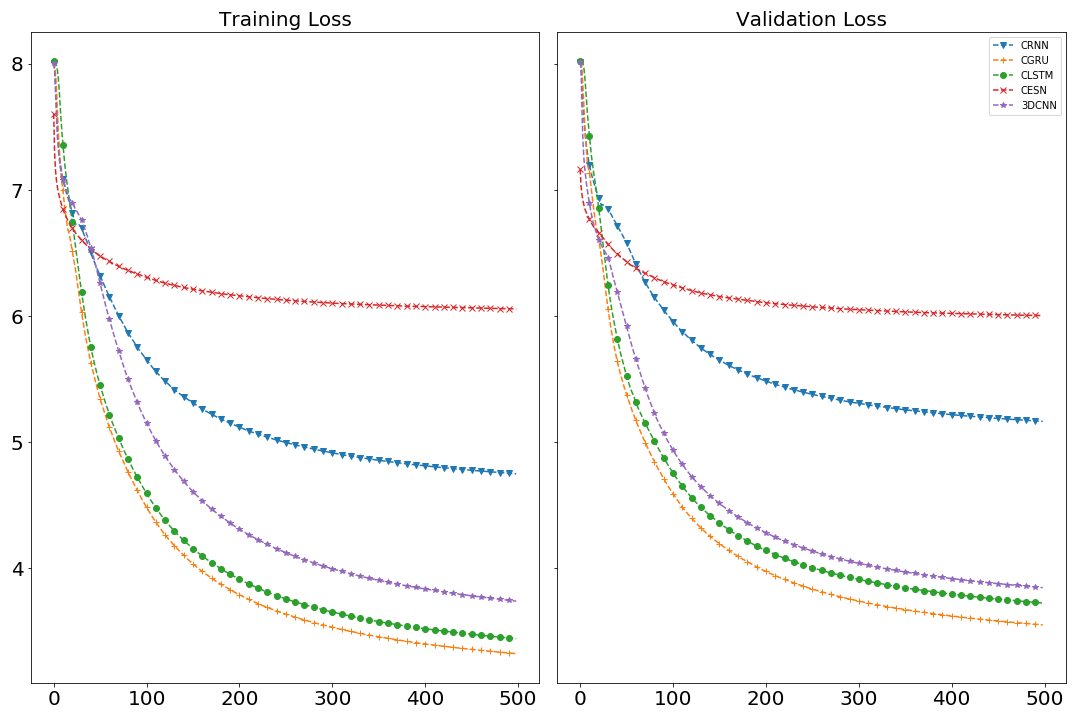
\includegraphics[width=1\textwidth]{Figure/Results/WEIZMANN_loss.png}
 \caption{WSD validation dataset loss curves for the CESN, CLSTM, CGRU, CRNN and 3DCNN.}
 \label{fig:WEIZMANN_model_loss}
\end{figure}


Figure~\ref{fig:WEIZMANN_model_perfomance} shows the precision, recall, $F_{1}Score$ and IoU of the CESN, CRNN, CLSTM, CGRU and 3DCNN on the validation set. All the models start with a lower performance with a single pass of the data, with further training the models performance increases and until it becomes constant at which further training does not make performance better or worse, this can be attributed a small learning rate as a result of the decaying rate.

In Figure~\ref{fig:WEIZMANN_model_perfomance}, the precision is higher than the recall for all the models, this implies that the models more sensitive to undersegmentation than oversegmentation~\cite{sigut2015over, troya2015unsupervised}, the latter can be due to the proportion of noise introduced by resizing the images or the scattered debris LS from previous time steps given that the data size in small. The CGRU has the highest precision and recall, followed by, CLSTM, 3DCNN, CRNN and lastly the CESN throughout the entire training procedure.

The $F_{1}Score$ is higher than the IoU in Figure~\ref{fig:WEIZMANN_model_perfomance}, this is because the models are penalized more for incorrectly classified segmentations boundaries. The CGRU has the highest $F_{1}Score$ followed by, CLSTM, 3DCNN, CRNN and lastly the CESN, but, when is comes to IoU 3DCNN is better monotonically than CLSTM with further training, this might be related to boundaries of the segmentation not clearly defined compare to the 3DCNN and the increased data samples compared to WSD.

The ESN and CRNN have the lowest IoU and $F_{1}Score$, this is because the CESN is more sensitive to the noise because of their inability to capture the long-term memory, therefore having a local spatial-temporal view of the LS evolution. While the, CLSTM, CGRU and 3DCNN are able to capture both the spatial-temporal evolution of the LS, therefore LS foreground pixels from earlier time step are now seen as noise, this is due to the ability of the CLSTM, CGRU and 3DCNN to capture the short-term and long-term memory, therefore having a global spatial-temporal view of the LS evolution.


\begin{figure}[H]
\centering
  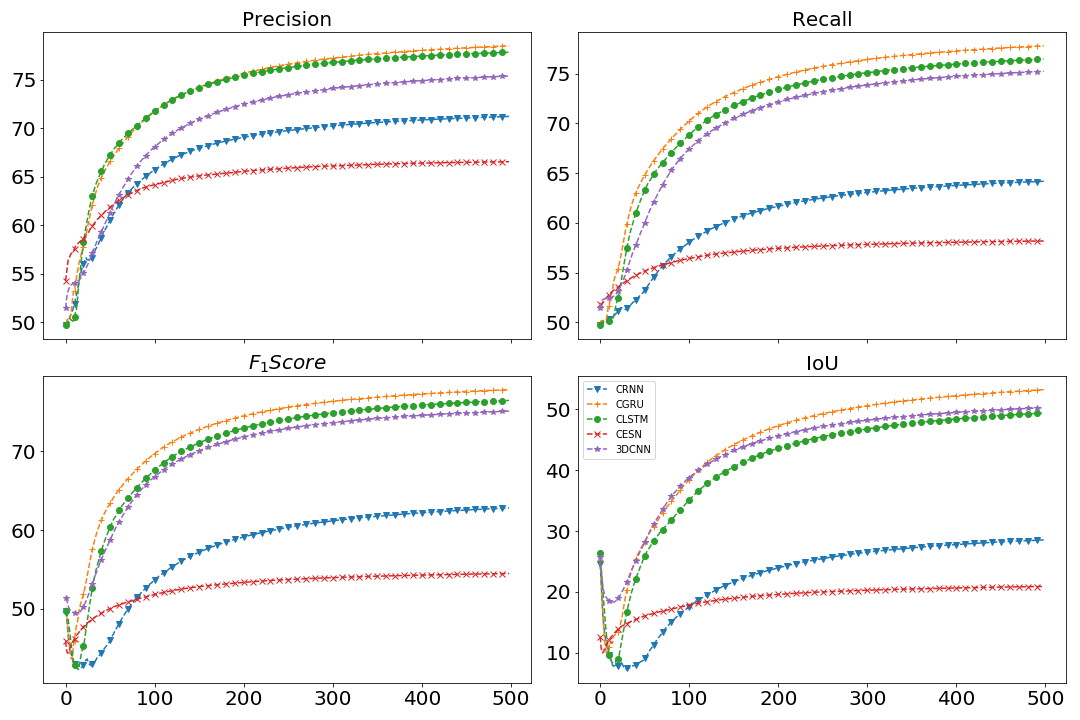
\includegraphics[width=1\textwidth]{Figure/Results/WEIZMANN_performance.png}
 \caption{WSD validation dataset learning curves for the CESN, CLSTM, CGRU, CRNN and 3DCNN.}
 \label{fig:WEIZMANN_model_perfomance}
\end{figure}

Table~\ref{tab:weizmann} shows the performance of the CESN, CRNN, CLSTM, CGRU and 3DCNN on the testing set. In addition, white noise is measured in order to determine the proportion of pixels that are considered to be random noise in the testing set, about 50\% of the the foreground pixels are noise as seen from the recall. Basically, this means the predictability of our models is benchmarked between being able to learn the spatio-temporal evolution of the LS or being a sequence of random numbers, therefore, cannot be predicted.  

The CESN is not performing better than random with a IoU of 21.9\%, and the CRNN with a IoU of 37.4\%. The CGRU with a IoU of 64.3\% outperforms all the other models, followed by,  the 3DCNN with a IoU of 61.9\% and CLSTM with a IoU of 61.6\%. The reason that CESN and CRNN are unable to effectively capture the spatio-temporal evolution of the LS as compare to the CGRU, CLSTM and 3DCNN, is due to their short-term memory, such that, for short-term memory the LS pixels are have similar characteristics to random noise, since the final segmentation state of the LS is dependent on both the information of the initial states and the current state of the LS, therefore, model which are able to capture both long-term and short-term memory have a advantage. 

\begin{table}[H]
\centering
 \caption{WSD testing set results. Here we compare various models and noise is also included.}
\resizebox{\linewidth}{!}{
    \begin{tabular}{cccccc}
    \hline
    \textbf{Methods} & \textbf{IoU} &  \textbf{Precision} &  \textbf{Recall} & \textbf{$F_{1}Score$}  \\
    \hline
    CGRU 	& 	\textbf{64.3}\% &	\textbf{76.8}\% &	\textbf{79.3} &	\textbf{76.8}\%\\
    3DCNN 	&	61.9\% &	75.5\% &	77.0\% &	76.0\% \\
    CLSTM 	& 	61.6\% &	75.5\% &	79.2\% &	75.7\% \\
    CRNN 	& 	37.4\% &	60.6\% &	66.5\% &	63.7\% \\
    CESN 	& 	21.9\% &	53.0\% &	63.2\% &	58.0\% \\
 	White Noise &35.4\% & 50.0\% &   50.0\%  & 48.2\% \\
    	\hline
    \end{tabular}}
    \label{tab:weizmann}
\end{table}


Figure~\ref{fig:sample_results_weizamann} shows samples segmentation the 1$^{st}$, 2$^{nd}$, 3$^{rd}$, 4$^{th}$, 5$^{th}$, 6$^{th}$ and 7$^{th}$ columns are the input images, ground-truth (i.e. LS), CESN, CRNN, CLSTM, CGRU and 3DCNN, respectively. The CESN is unable to capture the boundaries of the segmentation, this likely due to the noise. The CRNN, CLSTM and CGRU are able to capture the boundaries, however, suffer from over-segmentation as seen from a larger recall than precision in Table~\ref{tab:weizmann}.

\begin{figure}[H]
\centering
  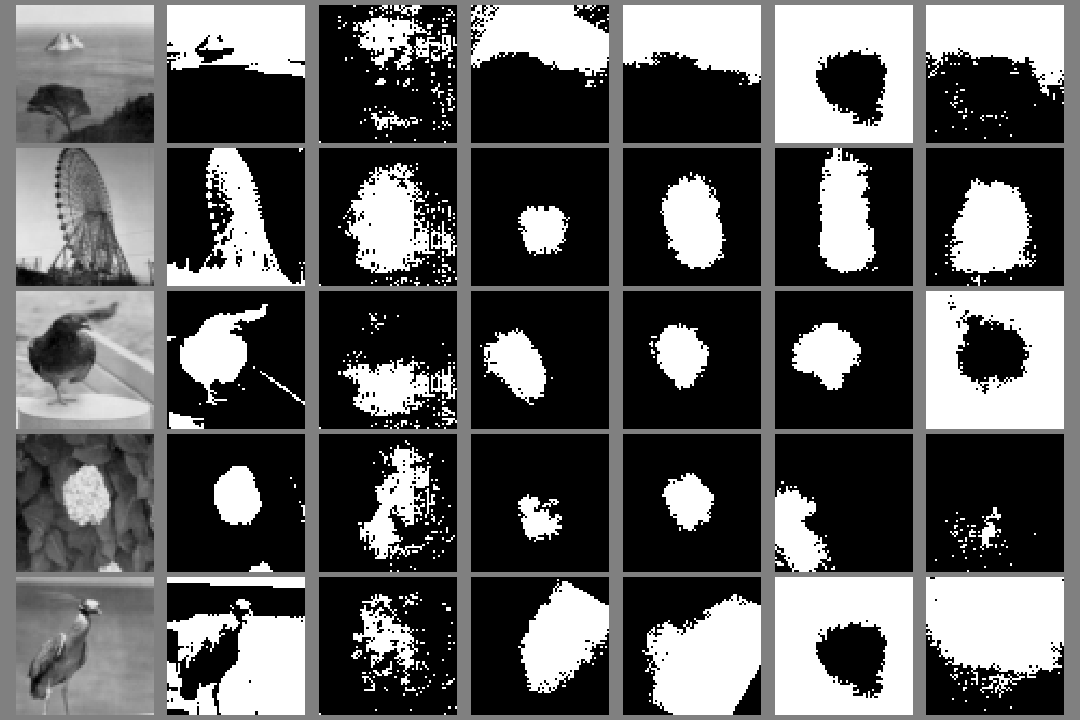
\includegraphics[width=1\textwidth]{Figure/Results/WEIZMANN_sample.png}
 \caption{WSD examples of iterative segmentation. $1^{st}$ column input, $2^{nd}$ Chan-Vese, $3^{rd}$ column CESN, $4^{th}$ CRNN, $5^{th}$ column CLSTM , $6^{th}$ column CGRU , $7^{th}$ column 3DCNN.}
 \label{fig:sample_results_weizamann}
\end{figure}

% Our results when compared to the state of the art when coming to reformulating LS as deep learning models

% \begin{figure}[H]
% \centering
%   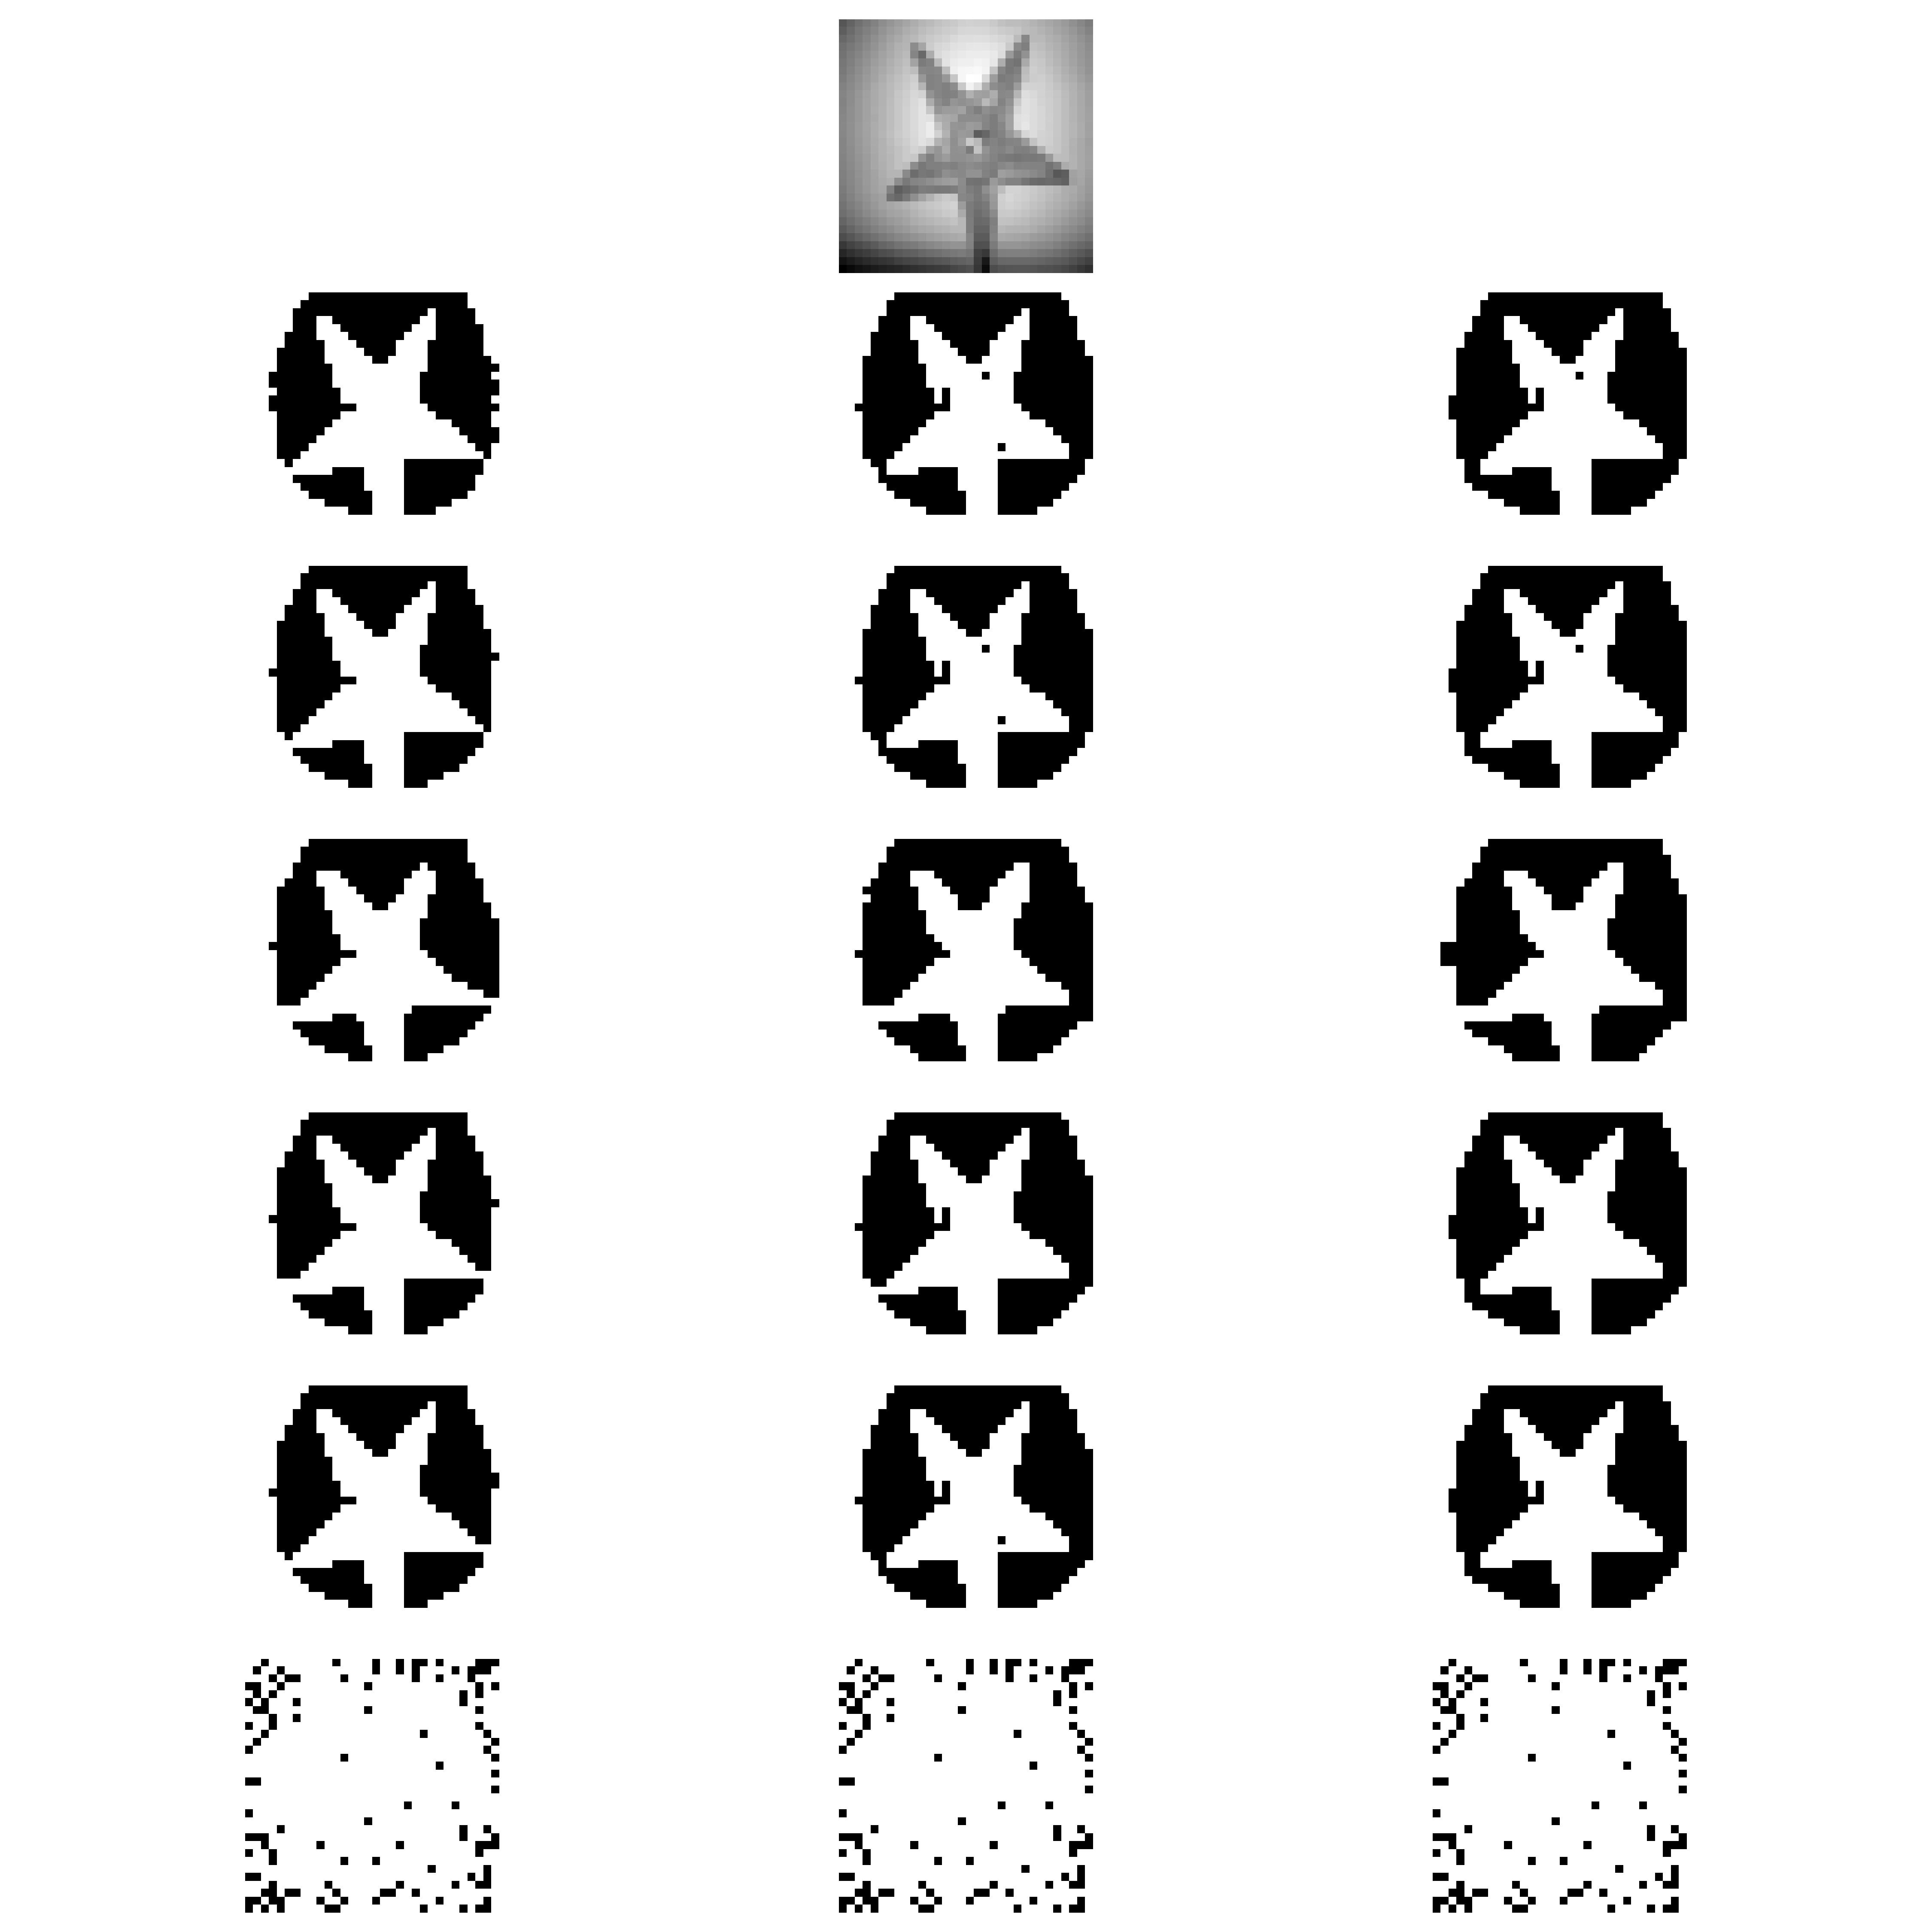
\includegraphics[width=1\linewidth]{Figure/Results/WEIZMANN_1_sample_images.png}
%  \caption{WSD sample iterative segmentation.  $1^{st}$ row input image, $2^{nd}$ row Chan-Vese, $3^{rd}$ row CESN ,  $4^{th}$ row CLSTM, $5^{th}$ row CGRU, $6^{th}$ row CRNN and  $7^{th}$ row 3DCNN at  \textit{1th, 10th and 50th} iteration, respectively.}
%  \label{fig:sample_results_weizmann}
% \end{figure}
\subsubsection{Conclusion}

The CGRU outperforms the 3DCNN, CLSTM and CRNN, this due is to that CGRU is less complex because of less gates than the CLSTM and the CLSTMs requires a lot of data for it to be able generalize. The CRNN is known for exploding and vanishing gradients~\cite{pascanu2013difficulty} and considering that the data size is small, the results are not surprising. The CESN is not performing better than random as seen in Table~\ref{tab:weizmann}, this is likely due to the fact the set the of parameters, especially the leaking and spectral radius, do not satisfy the echo state property mention in Section~\ref{sec:echo_state_property_and_spectral_radius}, and also optimizing  large reservoirs of orders of magnitude 10$^3$ is challenging~\cite{jaeger2001echo}. The CESN although is a efficient alternative to training RNNs, however, optimal performance is not guaranteed due to the number of hyperprameters that need to be optimized and therefore does not perform better than state of the art RNNs under this experiment.


% \newpage
% ========================================================================= %
% ========================================================================= %

\subsection{BSD}
\label{sec:BSD}

\subsubsection{Introduction}
In this experiment we used the Berkeley segmentation database, images in this dataset do not have well defined boundaries and can contains more than 2 overlapping objects. Therefore the database is more complex compared and has more samples than WSD database.

\subsubsection{Results And Discussion}

Table~\ref{table:BSD_hyperparameter} shows the optimal parameters for each model selected based on the performance of the models~\footnote{CESN, CRNN, CLSTM, CGRU and 3DCNN are all referred as \textbf{models} for brevity.} on the validation set. The input images are resized to 64$\times$64, therefore, the number of fully-connected units in and hidden units for the CESN, CRNN, CLSTM, CGRU and 3DCNN is 4096, and the optimal leaking rate, spectral radius, sparsity and input scaling for CESN are 0.113, 0.7, 0.8 and 0.5, respectively. The optimal parameters are chosen by maximizing the IoU on the validation set.

\begin{table}[H]
    \centering
        \caption{BSD optimal parameters for the CESN, CRNN, CLSTM, CGRU and 3DCNN}
    \resizebox{\linewidth}{!}{
    \begin{tabular}{ccccccc}
    \hline
    \textbf{Model} &  \textbf{Hidden size} & \textbf{Leaking rate} & \textbf{Sparsity} & \textbf{Spectral radius} & \textbf{Input scaling}\\
    \hline
      CESN   & 4096   & 0.113   &  0.8  &  0.7  & 0.5 \\
      CRNN   & 4096  & -         &  -  &  -  & -  \\
      CLSTM  & 4096   &           &  -  &  -  & -   \\
      CGRU   & 4096  & -      &  -  &  -  & -    \\
      CGRU   & 4096  & -      &  -  &  -  & -    \\

    \hline
    \end{tabular}}
    \label{table:BSD_hyperparameter}
\end{table}



Figure~\ref{fig:BSD_model_loss} shows the training and validation loss of the CESN, CRNN, CLSTM, CGRU and 3DCNN versus the number of epochs (i.e. data passes). The training and validation loss are decreasing with further training, and since the validation loss is slightly greater than training loss, this means that the models are able to generalise on unseen observation and mostly likely to not overfit on the training set, the reasons are twofold, 1) decaying learning rate which helps the models converge to local minima and avoid oscillations~\cite{you2019does}, 2) dropout connection with a probability of 50\% between the convolutional layers help with overfitting, especially when working deep learning models that have large number of parameters as the one considered in this study~\cite{hinton2012improving}.


All the models the loss is decreasing with different magnitudes, this is a direct indications of the ability of the models to learn the LS function, the CGRU has the lowest validation loss, followed by, CLSTM, 3DCNN, CRNN and lastly the CESN. The CESN has the lowest starting loss, however a lower rate of change in loss compared to CRNN, CLSTM, CGRU and 3DCNN. And CLSTM, CGRU and 3DCNN validation loss curves are close to each other, and exhibit similar trend, which means they are more likely to have the similar performance. These curves are used to monitor overfitting and underfitting during training, however, since we implemented early stopping to stop the training when overfitting occurs, overfitting is not likely to occur due to training, that is not to say it won't occur due to the model complexity.


% Figure~\ref{fig:BSD_model_loss} shows the training and validation  loss of the CESN, CRNN, CLSTM, CGRU and 3DCNN against the number of epochs. The training and validation loss are decreasing with further training, this means that the models are not overfitting on the training set, and for all the models the loss is decreasing with different magnitude, this is a direct indications of the ability of the models to learn the LS function, the CGRU has the lowest validation loss, followed by, CLSTM, 3DCNN, CRNN and lastly the CESN. The CESN has the lowest starting loss, however a lower rate of change in loss compared to CRNN, CLSTM, CGRU and 3DCNN. And CLSTM, CGRU and 3DCNN loss curves are close to each other, and exhibit similar trend, which means they are more likely to have the similar performance.

\begin{figure}[H]
\centering
  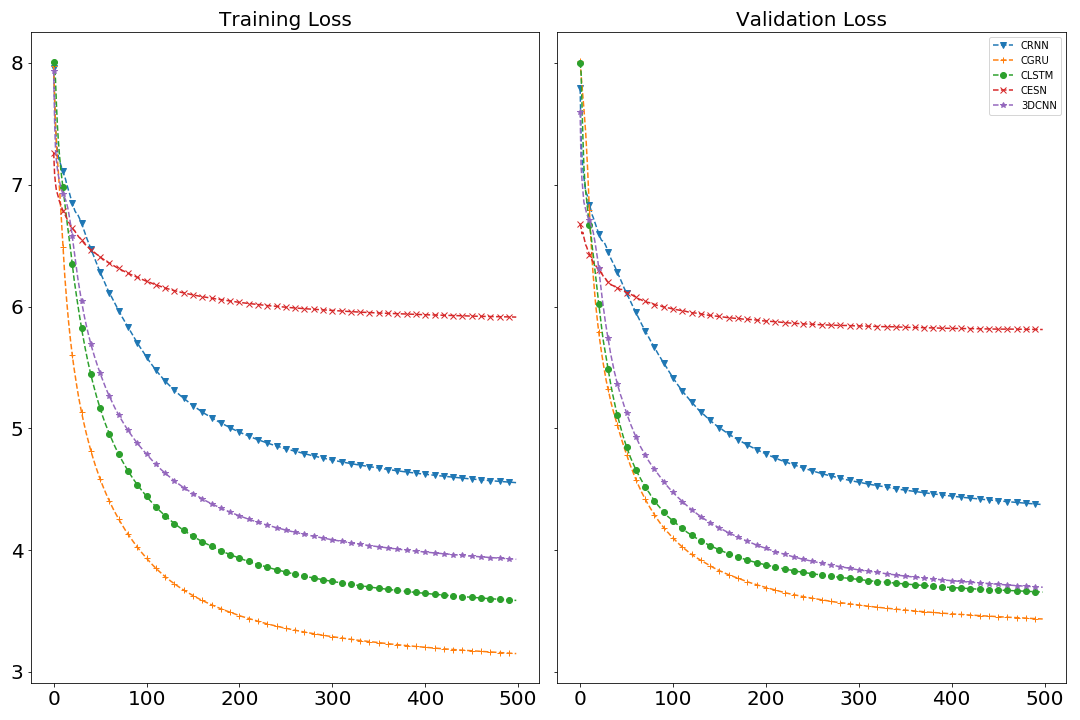
\includegraphics[width=1\textwidth]{Figure/Results/BSR_loss.png}
\caption{BSD dataset validadion loss curves for the CESN, CLSTM, CGRU, CRNN and 3DCNN.} \label{fig:BSD_model_loss}
\end{figure}

Figure~\ref{fig:BSD_model_perfomance} shows the precision, recall, $F_{1}Score$ and IoU of the CESN, CRNN, CLSTM, CGRU and 3DCNN on the validation set. All the models start with a lower performance with a single pass of the data, with further training the models performance increases and until it becomes constant at which further training does not make performance better or worse, this can be attributed a small learning rate as a result of the decaying rate.

In Figure~\ref{fig:BSD_model_perfomance}, the precision is higher than the recall for all the models, this implies that the models more sensitive to undersegmentation than oversegmentation~\cite{sigut2015over, troya2015unsupervised}, the latter can be due to the proportion of noise introduced by resizing the images or the scattered debris LS from previous time steps given that the data size in small. The CGRU has the highest precision and recall, followed by, CLSTM, 3DCNN, CRNN and lastly the CESN throughout the entire training process.

The $F_{1}Score$ is higher than the IoU in Figure~\ref{fig:BSD_model_perfomance}, this is because the models are penalized more for incorrectly classified segmentations boundaries. The CGRU has the highest $F_{1}Score$ followed by, CLSTM, 3DCNN, CRNN and lastly the CESN, but, when is comes to IoU 3DCNN is better than CLSTM, this might be related to boundaries of the segmentation not clearly defined compare to the 3DCNN. 

The ESN and CRNN have the lowest IoU and $F_{1}Score$, this is because the CESN is more sensitive to the noise because of their inability to capture the long-term memory, therefore having a local spatial-temporal view of the LS evolution. While the, CLSTM, CGRU and 3DCNN are able to capture both the spatial-temporal evolution of the LS, therefore LS foreground pixels from earlier time step are now seen as noise, this is due to the ability of the CLSTM, CGRU and 3DCNN to capture the short-term and long-term memory, therefore having a global spatial-temporal view of the LS evolution.



% Figure~\ref{fig:BSD_model_perfomance} shows the precision, recall, $F_{1}Score$ and IoU of the CESN, CRNN, CLSTM, CGRU and 3DCNN on the validation set. All the models start with a lower performance with a single pass of the data, with further training the models performance increases and until it becomes constant at which further training does not make performance better or worse, this is mostly due to the a small learning rate or size of the training data.

% Lets look at the precision and recall curves, the precision is higher than the recall for all the models, this means that the models are more likely to under-segment than over-segment the image, one major reason for this is due to the noise in relation to the number of training examples in the data, therefore the models ability to capture finer changes of the LS such that they are different from the noise is challenging. The CGRU has the highest precision and recall, followed by, CLSTM, 3DCNN, CRNN and lastly the CESN throughout the entire training process. 

% Now lets look at the $F_{1}Score$ and IoU, clearly the model are penalized more for incorrect classified segmentation, this is seen from $\approx$ 10\% higher $F_{1}Score$ than IoU. The CGRU has the highest $F_{1}Score$ has the highest  followed by, CLSTM, 3DCNN, CRNN and lastly the CESN, but, when is comes to IoU 3DCNN is better than CLSTM, this might be related to boundaries of the segmentation not clearly defined compare to the 3DCNN. The ESN has the worst IoU and $F_{1}Score$, this is because the CESN is more sensitive to the noise and therefore unable to capture the spatial evolution of the LS, while the other CRNN, CLSTM, CGRU and 3DCNN are able to capture both the spatial and temporal evolution of the LS.

\begin{figure}[H]
\centering
  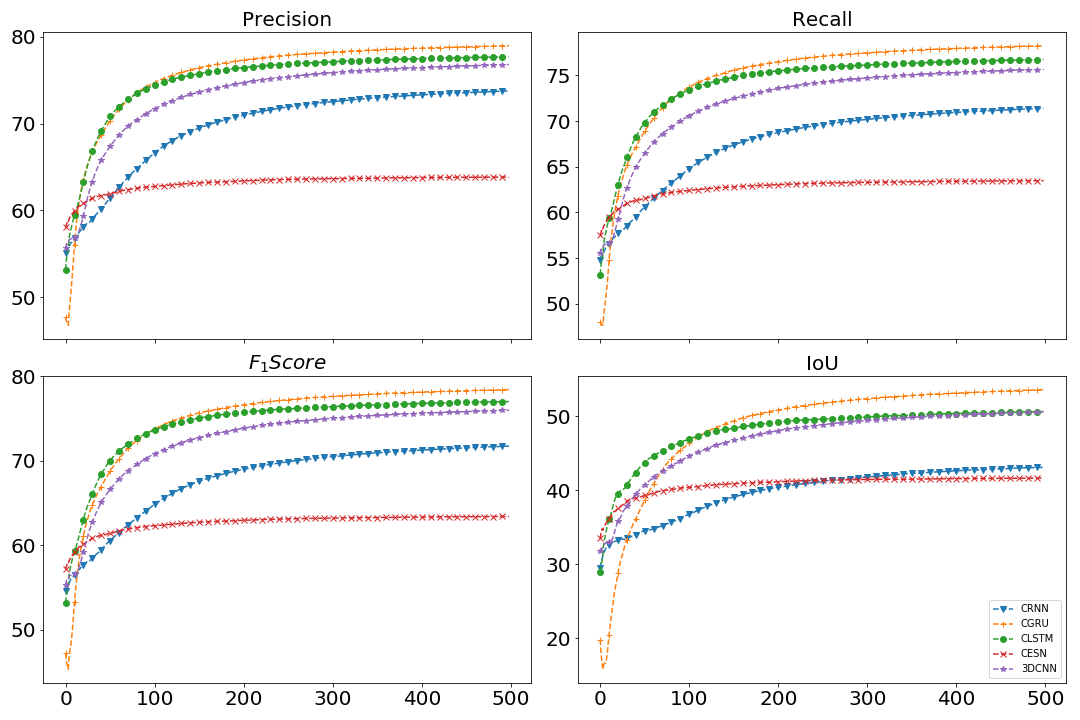
\includegraphics[width=1\textwidth]{Figure/Results/BSR_performance.png}
\caption{BSD dataset validation learning curves for the CESN, CLSTM, CGRU, CRNN and 3DCNN.} \label{fig:BSD_model_perfomance}
\end{figure}


Table~\ref{tab:bsd500} shows the performance of the CESN, CRNN, CLSTM, CGRU and 3DCNN on the testing set. In addition, white noise is measured in order to determine the proportion of pixels that are considered to be random noise in the testing set, about 50\% of the the foreground pixels are noise as seen from the recall. Basically, this means the predictability of our models is benchmarked between being able to learn the spatio-temporal evolution of the LS or being a sequence of random numbers, therefore, cannot be predicted.  

The CESN is not performing better than random with a IoU of 37.5\%. The CGRU with a IoU of 56.7\% outperforms all the other models, followed by, the CLSTM with a IoU of 54.8\%, 3DCNN with a IoU of 53.5\% and CRNN with a IoU of 49.7\% . Even with more data the CESN is still unable capture the spatio-temporal evolution of the LS as compare to the CGRU, CLSTM, CRNN and 3DCNN, is due to it's short-term memory, such that, for short-term memory the LS pixels are have similar characteristics to random noise, since the final segmentation state of the LS is dependent on both the information of the initial states and the current state of the LS, therefore, model which are able to capture both long-term and short-term memory have a advantage. More data certainly improved the CRNN segmentation results as seen in  Figure~\ref{fig:sample_results_BSD}.

% Table~\ref{tab:bsd500} shows the of the CESN, CRNN, CLSTM, CGRU and 3DCNN on the testing set. In addition, we added random noise to measure the proportion of noise in the testing set, about 50\% of the the foreground pixels are noise as seen from the recall. The CESN is doing worse than random noise with IoU of 37.5\%, and the CRNN with a IoU of 49.7\%. The top three performing model are CGRU IoU of 56.7\%, 3DCNN IoU of 53.5\% and CLSTM IoU of 54.8\%. On the testing set we can see that recall is larger than the precision, which means the models are over-segmenting the images, this may be due to over-fitting, given that the data samples are small.
 
\begin{table}[H]
\centering
\caption{BSD testing results. Here we compare various models and noise is also included.}
\resizebox{\linewidth}{!}{
    \begin{tabular}{cccccc}
    \hline
    \textbf{Method} & \textbf{IoU} &  \textbf{Precision} &  \textbf{Recall} & \textbf{$F_{1}Score$}           \\
    \hline
    CGRU 	& 	\textbf{56.7}\% &	\textbf{73.4}\% &	\textbf{76.1}\% &	\textbf{73.6}\% \\
    CLSTM 	& 	54.8\% &	71.1\% &	73.4\% &	71.4\% \\
    3DCNN 	& 	53.5\% &	70.7\% &	73.1\% &	71.0\% \\
    CRNN 	& 	49.7\% &	69.4\% &	71.8\% &	70.1\% \\
    CESN 	& 	37.5\% &	60.0\% &	61.1\% &	62.0\% \\
 	White Noise  &  44.9\%   & 50.0\%  &   50.0\% &  43.4\%    \\
    	\hline
    \end{tabular}}
    \label{tab:bsd500}
\end{table}

Figure~\ref{fig:sample_results_BSD} shows samples segmentation the 1$^{st}$, 2$^{nd}$, 3$^{rd}$, 4$^{th}$, 5$^{th}$, 6$^{th}$ and 7$^{th}$ columns are the input images, ground-truth (i.e. LS), CESN, CRNN, CLSTM, CGRU and 3DCNN, respectively. The CESN is unable to capture the boundaries of the segmentation, the noise has an impact on segmentation results as seen by the disjoint regions. The CRNN, CLSTM and CGRU are able to capture the boundaries especially for non-overlapping objects, but due to over-segmentation as seen from a larger recall than precision in Table~\ref{tab:bsd500}, the boundaries are not well-defined.

% Figure~\ref{fig:sample_results_BSD} shows samples segmentation, first, second, third, fourth, fifth, sixth and seventh columns are the input images, ground-truth (i.e. LS), CESN, CRNN, CLSTM, CGRU and 3DCNN, respectively. The CESN is unable to capture the boundaries of the segmentation, this likely due to the noise. The CRNN, CLSTM, 3DCNN and CGRU are able to capture the boundaries for non overlapping objects, however, suffer from over-segmentation, and they are able to segment, and the segmentation boundaries are over-segmented . Dealing with overlapping objects
% is a challenge for all the models.

\begin{figure}[H]
\centering
  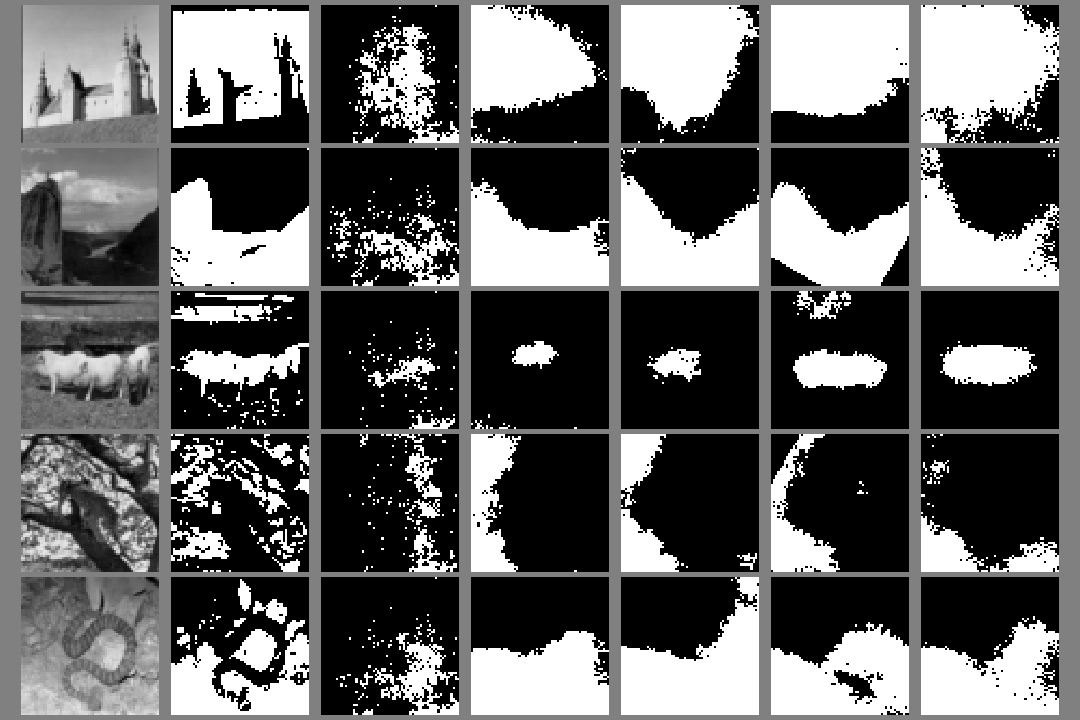
\includegraphics[width=1\linewidth]{Figure/Results/BSR_sample.png}
%  \caption{Segmentation  BSD. $1^{st}$ row input image, $2^{nd}$ row Chan-Vese, $3^{rd}$ row CESN ,  $4^{th}$ row CLSTM, $5^{th}$ row CGRU, $6^{th}$ row CRNN and  $7^{th}$ row 3DCNN at  \textit{1th, 10th and 50th} iteration, respectively.}
 \caption{BSD examples of iterative segmentation. $1^{st}$ column input, $2^{nd}$ Chan-Vese, $3^{rd}$ column CESN, $4^{th}$ CRNN, $5^{th}$ column CLSTM , $6^{th}$ column CGRU , $7^{th}$ column 3DCNN.}
 \label{fig:sample_results_BSD}
\end{figure}



% \begin{figure}[H]
% \centering
%   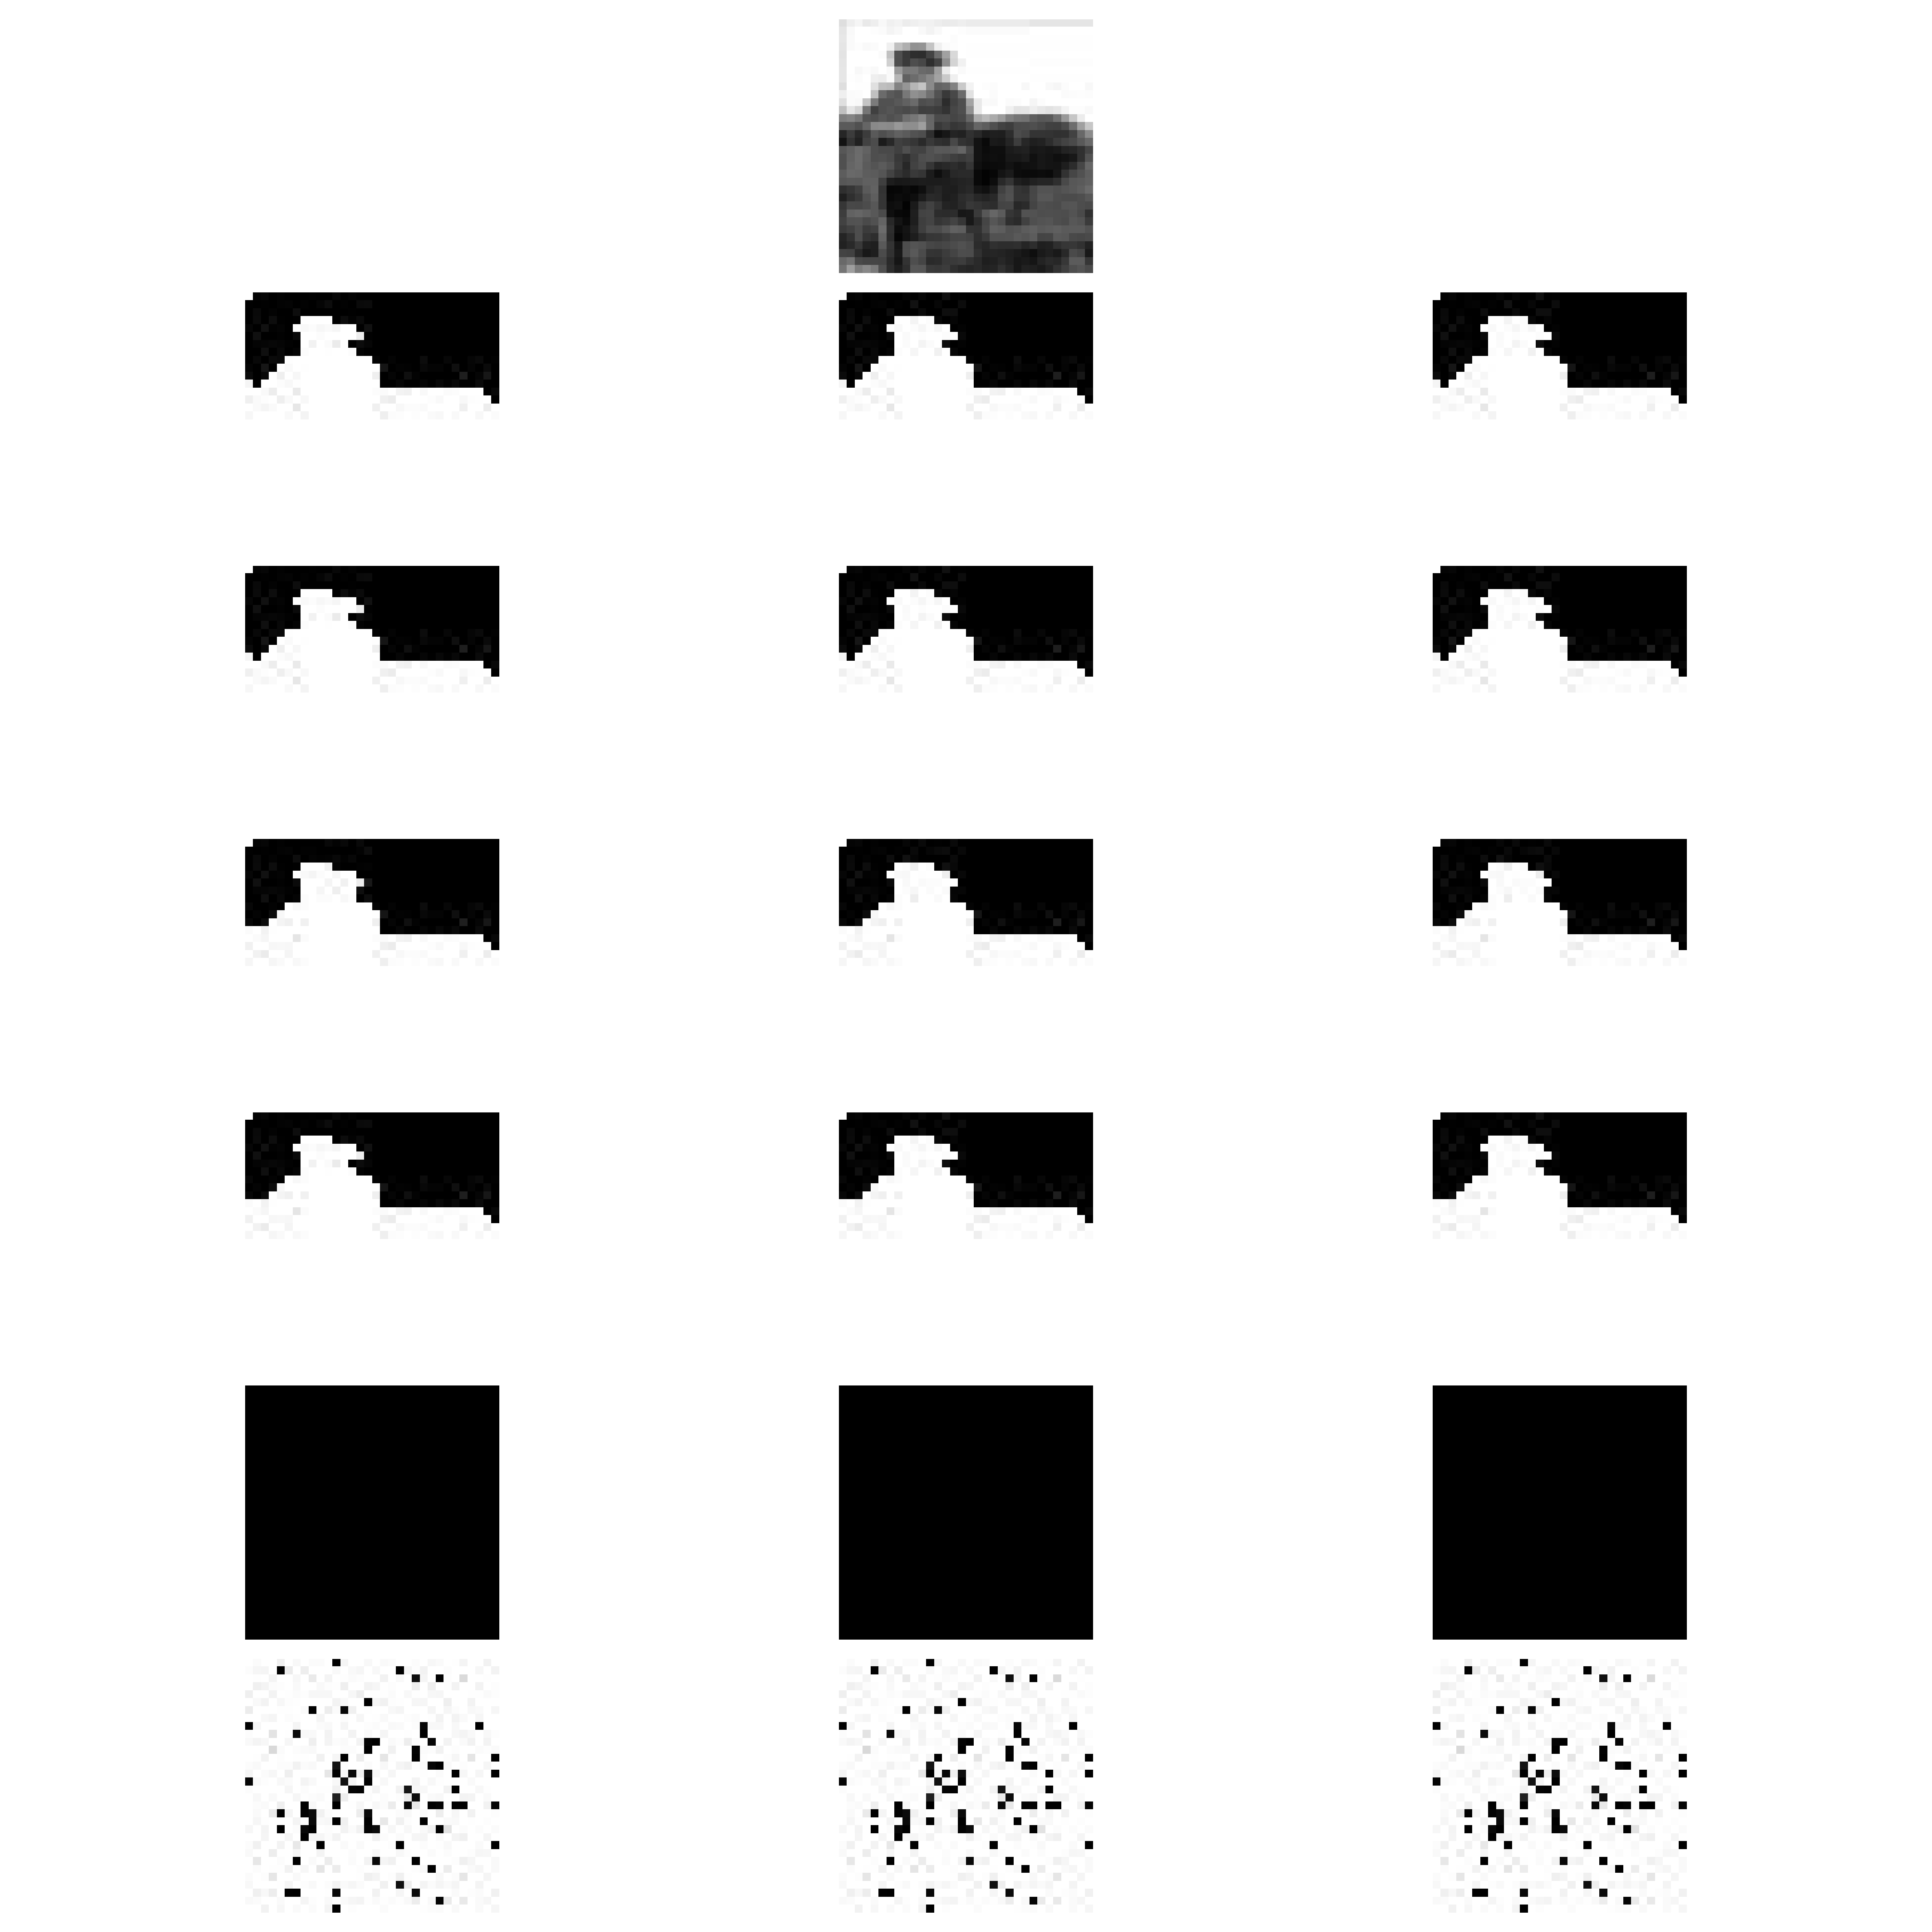
\includegraphics[width=1\linewidth]{Figure/Results/BSR_25_sample_images.png}
%  \caption{Segmentation  BSD. $1^{st}$ row input image, $2^{nd}$ row Chan-Vese, $3^{rd}$ row CESN ,  $4^{th}$ row CLSTM, $5^{th}$ row CGRU, $6^{th}$ row CRNN and  $7^{th}$ row 3DCNN at  \textit{1th, 10th and 50th} iteration, respectively.}
%  \label{fig:sample_results_BSD}
% \end{figure}

% The CGRU outperforms the 3DCNN, CLSTM and CRNN, this due is to that CGRU is less complex because of less gates than the CLSTM and the CLSTMs requires a lot of data for it to be able generalize. The CRNN is known for exploding and vanishing gradients~\cite{pascanu2013difficulty} and considering that the data size, the results are not surprising. The CESN is still not performing better than chance as seen in Table~\ref{tab:bsd500}, this is likely due to the fact the set the of parameters, especially the leaking and spectral radius, do not satisfy the echo state property mention in Section~\ref{sec:echo_state_property_and_spectral_radius}, and also optimizing  large reservoirs of orders of magnitude 10$^3$ is challenging~\cite{jaeger2001echo}.  

\subsubsection{Conclusion}

The CGRU outperforms the 3DCNN, CLSTM and CRNN. The additional data samples improved the CGRU, 3DCNN, CLSTM and CRNN segmentation resutls when compared to the previous experiment in Section~\ref{sec:Weizmann}, with a exception of the CESN. 

The CESN is still not performing better than random as seen in Table~\ref{tab:bsd500}, this is due to the selected set of parameters do not satisfy the echo state property mention in Section~\ref{sec:echo_state_property_and_spectral_radius}, especially the leaking and spectral radius, and also optimizing large reservoirs of orders of magnitude 10$^3$ is challenging~\cite{jaeger2001echo}. The CESN although is a efficient alternative to training RNNs, however, optimal performance is not guaranteed due to the number of hyperprameters that need to be optimized and therefore does not perform better than state-of-the-art RNNs under the conditions of this experiment.

\newpage

% ========================================================================= %
% ========================================================================= %

\subsection{CIFAR-10}
\label{sec:cifar_10}

\subsubsection{Introduction}

In this experiment, we used the CIFAR-10 database, this database is much more complex that the previous database mentioned above, the additional complexity is due number of different classes and significantly larger sample than the BSD and WSD.

\subsubsection{Result And Discussion}
Table~\ref{table:cifar_10_hyperparameter} shows the optimal parameters for each model selected based on the performance of the models~\footnote{CESN, CRNN, CLSTM, CGRU and 3DCNN are all referred as \textbf{models} for brevity.} on the validation set. The input images are resized to 64$\times$64, therefore, the number of fully-connected units in and hidden units for the CESN, CRNN, CLSTM, CGRU and 3DCNN is 4096, and the optimal leaking rate, spectral radius, sparsity and input scaling for CESN are 0.01, 0.7, 0.2 and 1, respectively. The optimal parameters are chosen by maximizing the IoU on the validation set.

\begin{table}[!htb]
    \centering
        \caption{CIFAR-10 dataset optimal parameters for the CESN, CRNN, CLSTM, CGRU and 3DCNN}
    \resizebox{\linewidth}{!}{
    \begin{tabular}{lllllll}
    \hline
    \textbf{Model} &  \textbf{Hidden size} & \textbf{Leaking rate} & \textbf{Sparsity} & \textbf{Spectral radius} & \textbf{Input scaling}\\
    \hline
      CESN  & 4096  & 0.01  & 0.2  &  0.9  & 1.0    \\
      CRNN  & 4096 & -  & -  &  -  & -             \\
      CLSTM & 4096  &    & -  &  -  & -            \\
      CGRU  & 4096 & -  & -  &  -  & -              \\
      3DCNN  & 4096 & -  & -  &  -  & -              \\
    \hline
    \end{tabular}}
    \label{table:cifar_10_hyperparameter}
\end{table}

Figure~\ref{fig:cifar_10_model_loss} shows the training and validation loss of the CESN, CRNN, CLSTM, CGRU and 3DCNN versus the number of epochs (i.e. data passes). The training and validation loss are decreasing with further training, and since the validation loss is slightly greater than training loss, this means that the models are able to generalise on unseen observation and mostly likely to not overfit on the training set, the reasons are twofold, 1) decaying learning rate which helps the models converge to local minima and avoid oscillations~\cite{you2019does}, 2) dropout connection with a probability of 50\% between the convolutional layers help with overfitting, especially when working deep learning models that have large number of parameters as the one considered in this study~\cite{hinton2012improving} 3) training with more data.


All the models the loss is decreasing with different magnitudes, this is a direct indications of the ability of the models to learn the LS function, the CGRU has the lowest validation loss, followed by, CLSTM, 3DCNN, CRNN and lastly the CESN. The CESN has the lowest starting loss, however a lower rate of change in loss compared to CRNN, CLSTM, CGRU and 3DCNN. And CLSTM, CGRU and 3DCNN validation loss curves are very close to each other, and exhibit similar trend, which means they are more likely to have the similar performance. These curves are used to monitor overfitting and underfitting during training, however, since we implemented early stopping to stop the training when overfitting occurs, overfitting is not likely to occur due to training, that is not to say it won't occur due to the model complexity. The CESN training and validation loss are almost equal, which is a hallmark of overfitting, however, without further training beyond 500 epoch we are unable to validate this assumption.


\begin{figure}[H]
\centering
  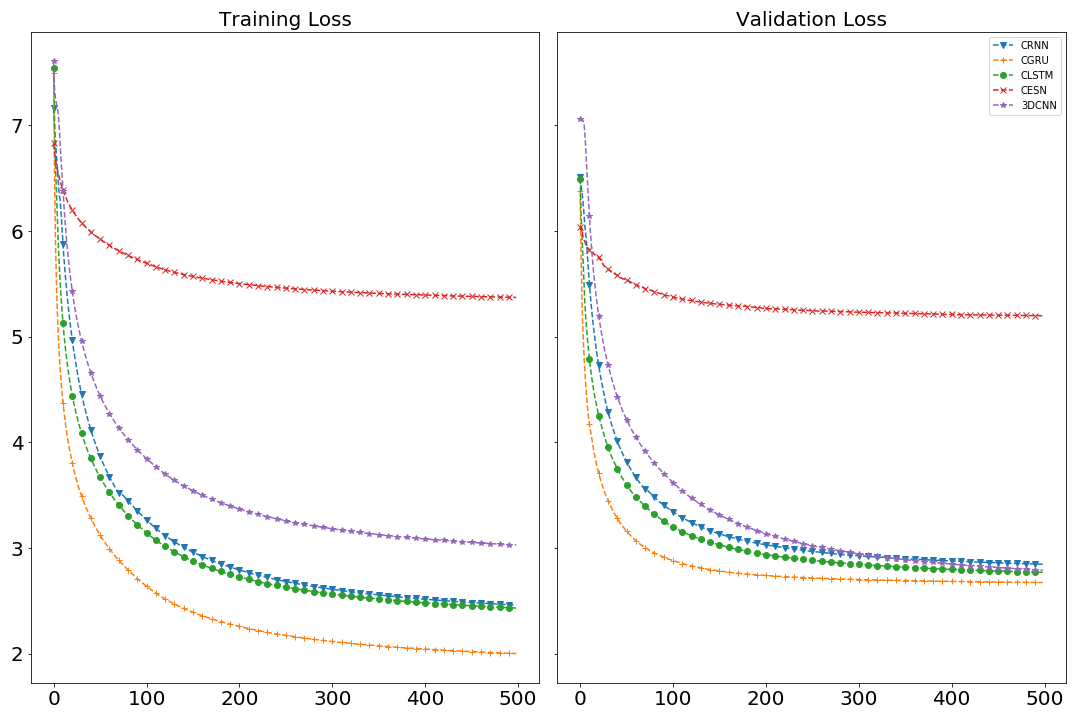
\includegraphics[width=1\textwidth]{Figure/Results/CIFAR_10_loss.png}
\caption{CIFAR-10 validation dataset loss curves for the CESN, CLSTM, CGRU, CRNN and 3DCNN}
 \label{fig:cifar_10_model_loss}
\end{figure}

Figure~\ref{fig:cifar_10_model_perfomance} shows the precision, recall, $F_{1}Score$ and IoU of the CESN, CRNN, CLSTM, CGRU and 3DCNN on the validation set. All the models start with a lower performance with a single pass of the data, with further training the models performance increases and until it becomes constant at which further training does not make performance better or worse, this can be attributed a small learning rate as a result of the decaying rate.

In Figure~\ref{fig:cifar_10_model_perfomance}, the precision is slightly higher than the recall for all the models, this implies that the models slightly more sensitive to undersegmentation than oversegmentation~\cite{sigut2015over, troya2015unsupervised}, the latter can be due to the proportion of noise introduced by up-resizing the images. The CGRU has the highest precision and recall, followed by, CLSTM, 3DCNN, CRNN and lastly the CESN throughout the entire training process. The most interesting observation, is the CGRU, CLSTM, CRNN and 3DCNN converge towards a single recall and precision, this is not surprising, since these models require large amounts of data in order to achieve state-of-the-art results.

The $F_{1}Score$ is higher than the IoU in Figure~\ref{fig:cifar_10_model_perfomance}, this is because the models are penalized more for incorrectly classified segmentations boundaries. %The CGRU has the highest $F_{1}Score$ followed by, CRNN, CLSTM, 3DCNN and lastly the CESN.  


The ESN have the lowest IoU and $F_{1}Score$, this is because the CESN is is still sensitive to the noise because of their inability to capture the long-term memory even with more training data, therefore having a local spatial-temporal view of the LS evolution. While the, CLSTM, CGRU, CRNN and 3DCNN are able to capture both the spatial-temporal evolution of the LS, therefore LS foreground pixels from earlier time step are now seen as noise, this is due to the ability of the CLSTM, CGRU and 3DCNN to capture the short-term and long-term memory, therefore having a global spatial-temporal view of the LS evolution. In contrast to the CRNN exponentially improves in performance with more data.




% Figure~\ref{fig:cifar_10_model_perfomance} shows the precision, recall, $F_{1}Score$ and IoU of the CESN, CRNN, CLSTM, CGRU and 3DCNN on the validation set. All the models start with a lower performance with a single pass of the data, with further training the models performance increases and until it becomes constant at which further training does not make performance better or worse, this is mostly due to the a small learning rate or size of the training data.

% Lets look at the precision and recall curves, the precision is sightly higher than the recall for all the models, this means that the models are more likely to under-segment than over-segment the image, therefore the models ability to capture finer changes of the LS such that they are different from the noise is challenging. The CGRU has the highest precision and recall, followed by, CLSTM, CRNN, 3DCNN and lastly the CESN throughout the entire training process. The most interesting observation, is the CGRU, CLSTM, CRNN and  3DCNN converge towards a single recall and precision, this is not surprising, since these model require large amounts of data in order to achieve state of the art results. The number of parameters of the CESN make it difficult to find the optimal parameters such the echo state property is satisfied, which then lead to sub-optimal performance.

% Now lets look at the $F_{1}Score$ and IoU, clearly the modes are slightly penalized more for incorrect classified segmentation, this is seen from $\approx$ 5\% higher $F_{1}Score$ than IoU. The CGRU has the highest $F_{1}Score$ has the highest  followed by, CLSTM, 3DCNN, CRNN and lastly the CESN, but, when is comes to IoU 3DCNN is better than CLSTM, this might be related to boundaries of the segmentation not clearly defined compare to the 3DCNN. The ESN has the worst IoU and $F_{1}Score$, this is because the CESN is more sensitive to the noise and therefore unable to capture the spatial evolution of the LS, while the other CRNN, CLSTM, CGRU and 3DCNN are able to capture both the spatial and temporal evolution of the LS.

\begin{figure}[H]
\centering
  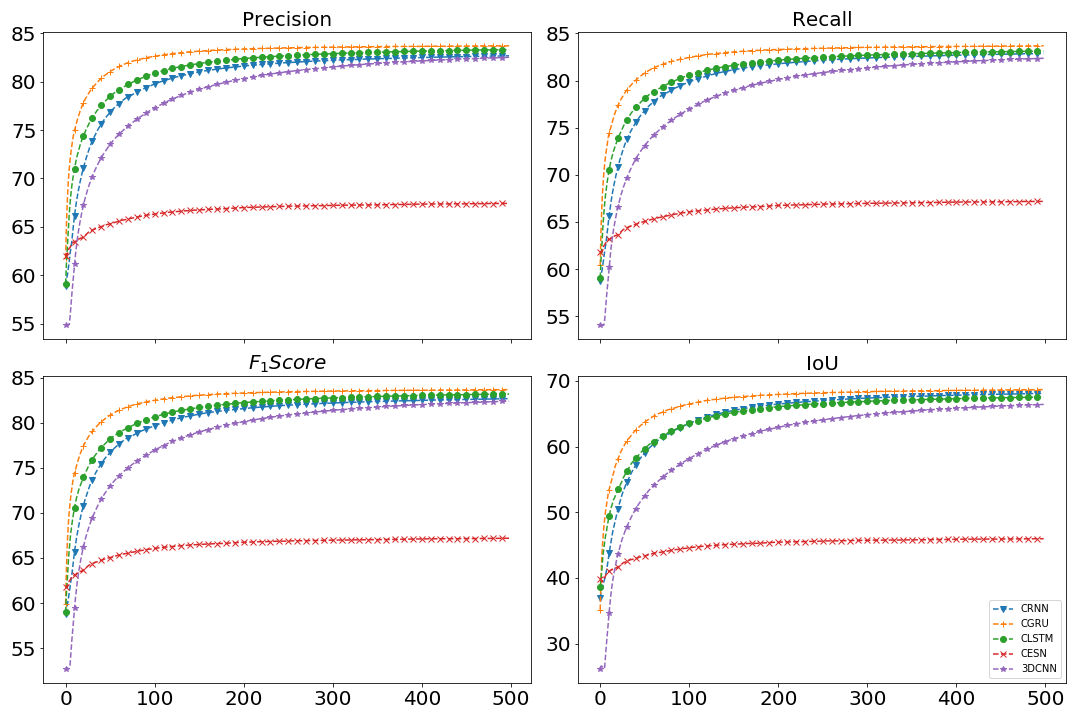
\includegraphics[width=1\textwidth]{Figure/Results/CIFAR_10_performance.png}
\caption{CIFAR-10 validation dataset learning curves for the CESN, CLSTM, CGRU, CRNN and 3DCNN}
 \label{fig:cifar_10_model_perfomance}
\end{figure}

Table~\ref{tab:cifar_10} shows the performance of the CESN, CRNN, CLSTM, CGRU and 3DCNN on the testing set. In addition, white noise is measured in order to determine the proportion of pixels that are considered to be random noise in the testing set, about 50\% of the the foreground pixels are noise as seen from the recall. Basically, this means the predictability of our models is benchmarked between being able to learn the spatio-temporal evolution of the LS or being a sequence of random numbers, therefore, cannot be predicted.  

The CESN is performing better than random with a IoU of 44.7\%. The CLSTM with a IoU of 68.8\% outperforms all the other models, followed by, the 3DCNN with a IoU of 68.7\%, CGRU with a IoU of 68.3\% and CRNN with a IoU of 68.0\% . Even with a significant increase in data the CESN is still unable capture the spatio-temporal evolution of the LS as compare to the CGRU, CLSTM, CRNN and 3DCNN, due to overfitting  because of it's short-term memory, such that, for short-term memory the LS pixels are have similar characteristics to random noise, since the final segmentation state of the LS is dependent on both the information of the initial states and the current state of the LS, therefore, model which are able to capture both long-term and short-term memory have a advantage. 

% Table~\ref{tab:cifar_10} shows the of the CESN, CRNN, CLSTM, CGRU and 3DCNN on the testing set. In addition, we added random noise to measure the proportion of noise in the testing set, about 50\% of the the foreground pixels are noise as seen from the recall. The CESN is performing better than random noise with IoU of 44.9\%, and the CRNN with a IoU of 68\%. The top three performing model are CLSTM IoU of 68.8\%, 3DCNN IoU of 68.7\% and CGRU IoU of 68.0\%. On the testing set we can see that recall is larger than the precision, which means the models are over-segmenting the images, this may be due to over-fitting or the upsampling $32\times32 \rightarrow 64\times64$ of the images which may introduced artifacts not part of the LS evolution.
 
\begin{table}[H]
\centering
\caption{CIFAR-10 testing results. Here we compare various models and noise is also included.}
\resizebox{\linewidth}{!}{
    \begin{tabular}{cccccc}
    \hline
    \textbf{Method} & \textbf{IoU} &  \textbf{Precision} &  \textbf{Recall} & \textbf{$F_{1}Score$}   \\
    \hline
    CLSTM 	&  	\textbf{68.8}\% 	&\textbf{82.8}\% 	&\textbf{83.8}\% 	& \textbf{82.5}\%\\
    3DCNN 	& 	68.7\% 	&82.5\% 	&83.4\% 	& 82.2\%\\
    CGRU 	& 	68.3\% 	&82.4\% 	&83.0\% 	& 82.2\%\\
    CRNN 	& 	68.0\% 	&81.9\% 	&82.9\% 	& 81.9\%\\
    CESN 	& 	44.9\% 	&65.1\% 	&65.7\% 	& 66.4\%\\
 	White Noise   & 30.3\%    & 50.0\%   &  50.0\%    &  49.5\%            \\
    	\hline
    \end{tabular}}
    \label{tab:cifar_10}
\end{table}

Figure~\ref{fig:sample_results_cifar10} shows samples segmentation the 1$^{st}$, 2$^{nd}$, 3$^{rd}$, 4$^{th}$, 5$^{th}$, 6$^{th}$ and 7$^{th}$ columns are the input images, ground-truth (i.e. LS), CESN, CRNN, CLSTM, CGRU and 3DCNN, respectively. We observe moderate overfitting characteristics, this is seen by the checkerbox structures in Figure~\ref{fig:sample_results_BSD}, since the LS is initialized as checkerbox, therefore this structures are common in all the samples in the data and the models are more likely to memorize these type of structures. 


The CESN is unable to capture the boundaries of the segmentation, although it was able to separate the plane from the back in 5$^{th}$ row. The CRNN, CLSTM , CGRU and 3DCNN are able to capture the boundaries, but due to over-segmentation as seen from a larger recall than precision in Table~\ref{tab:bsd500}, the boundaries are not well-defined, this could be due to that the training was stopped prematurely.

% Figure~\ref{fig:sample_results_cifar10} shows samples segmentation, first, second, third, fourth, fifth, sixth and seventh columns are the input images, ground-truth (i.e. LS), CESN, CRNN, CLSTM, CGRU and 3DCNN, respectively. The CESN is unable to capture the time evolution of the LS, this seen from the cheakerbox like structures, which are present in the earlier time steps of the LS. The CRNN, CLSTM, 3DCNN and CGRU are able to capture the boundaries for non overlapping objects, however, suffer from over-segmentation, and they are able to segment, and the segmentation boundaries are over-segmented. The CRNN, CLSTM, CGRU and 3DCNN as seen in the images are able to capture the temporal evolution of the LS.

\begin{figure}[H]
\centering
  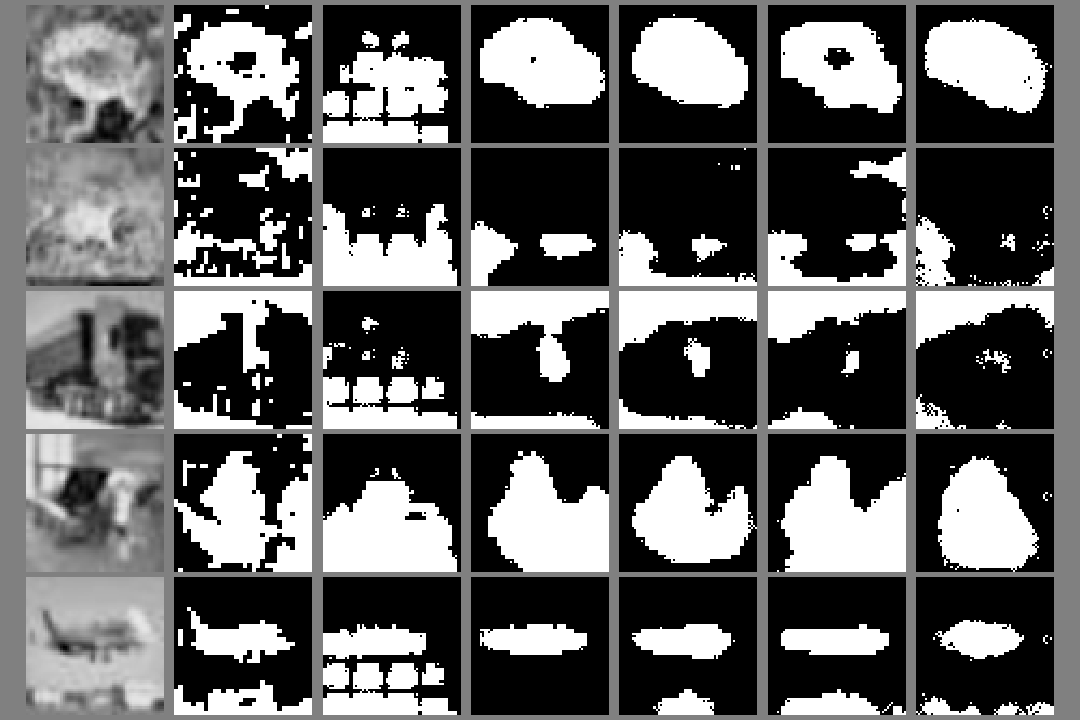
\includegraphics[width=1\linewidth]{Figure/Results/CIFAR_10_sample.png}
  \caption{CIFAR-10 examples of iterative segmentation. $1^{st}$ column input, $2^{nd}$ Chan-Vese, $3^{rd}$ column CESN, $4^{th}$ CRNN, $5^{th}$ column CLSTM , $6^{th}$ column CGRU , $7^{th}$ column 3DCNN.}
 \label{fig:sample_results_cifar10}
\end{figure}

% \begin{figure}[H]
% \centering
%   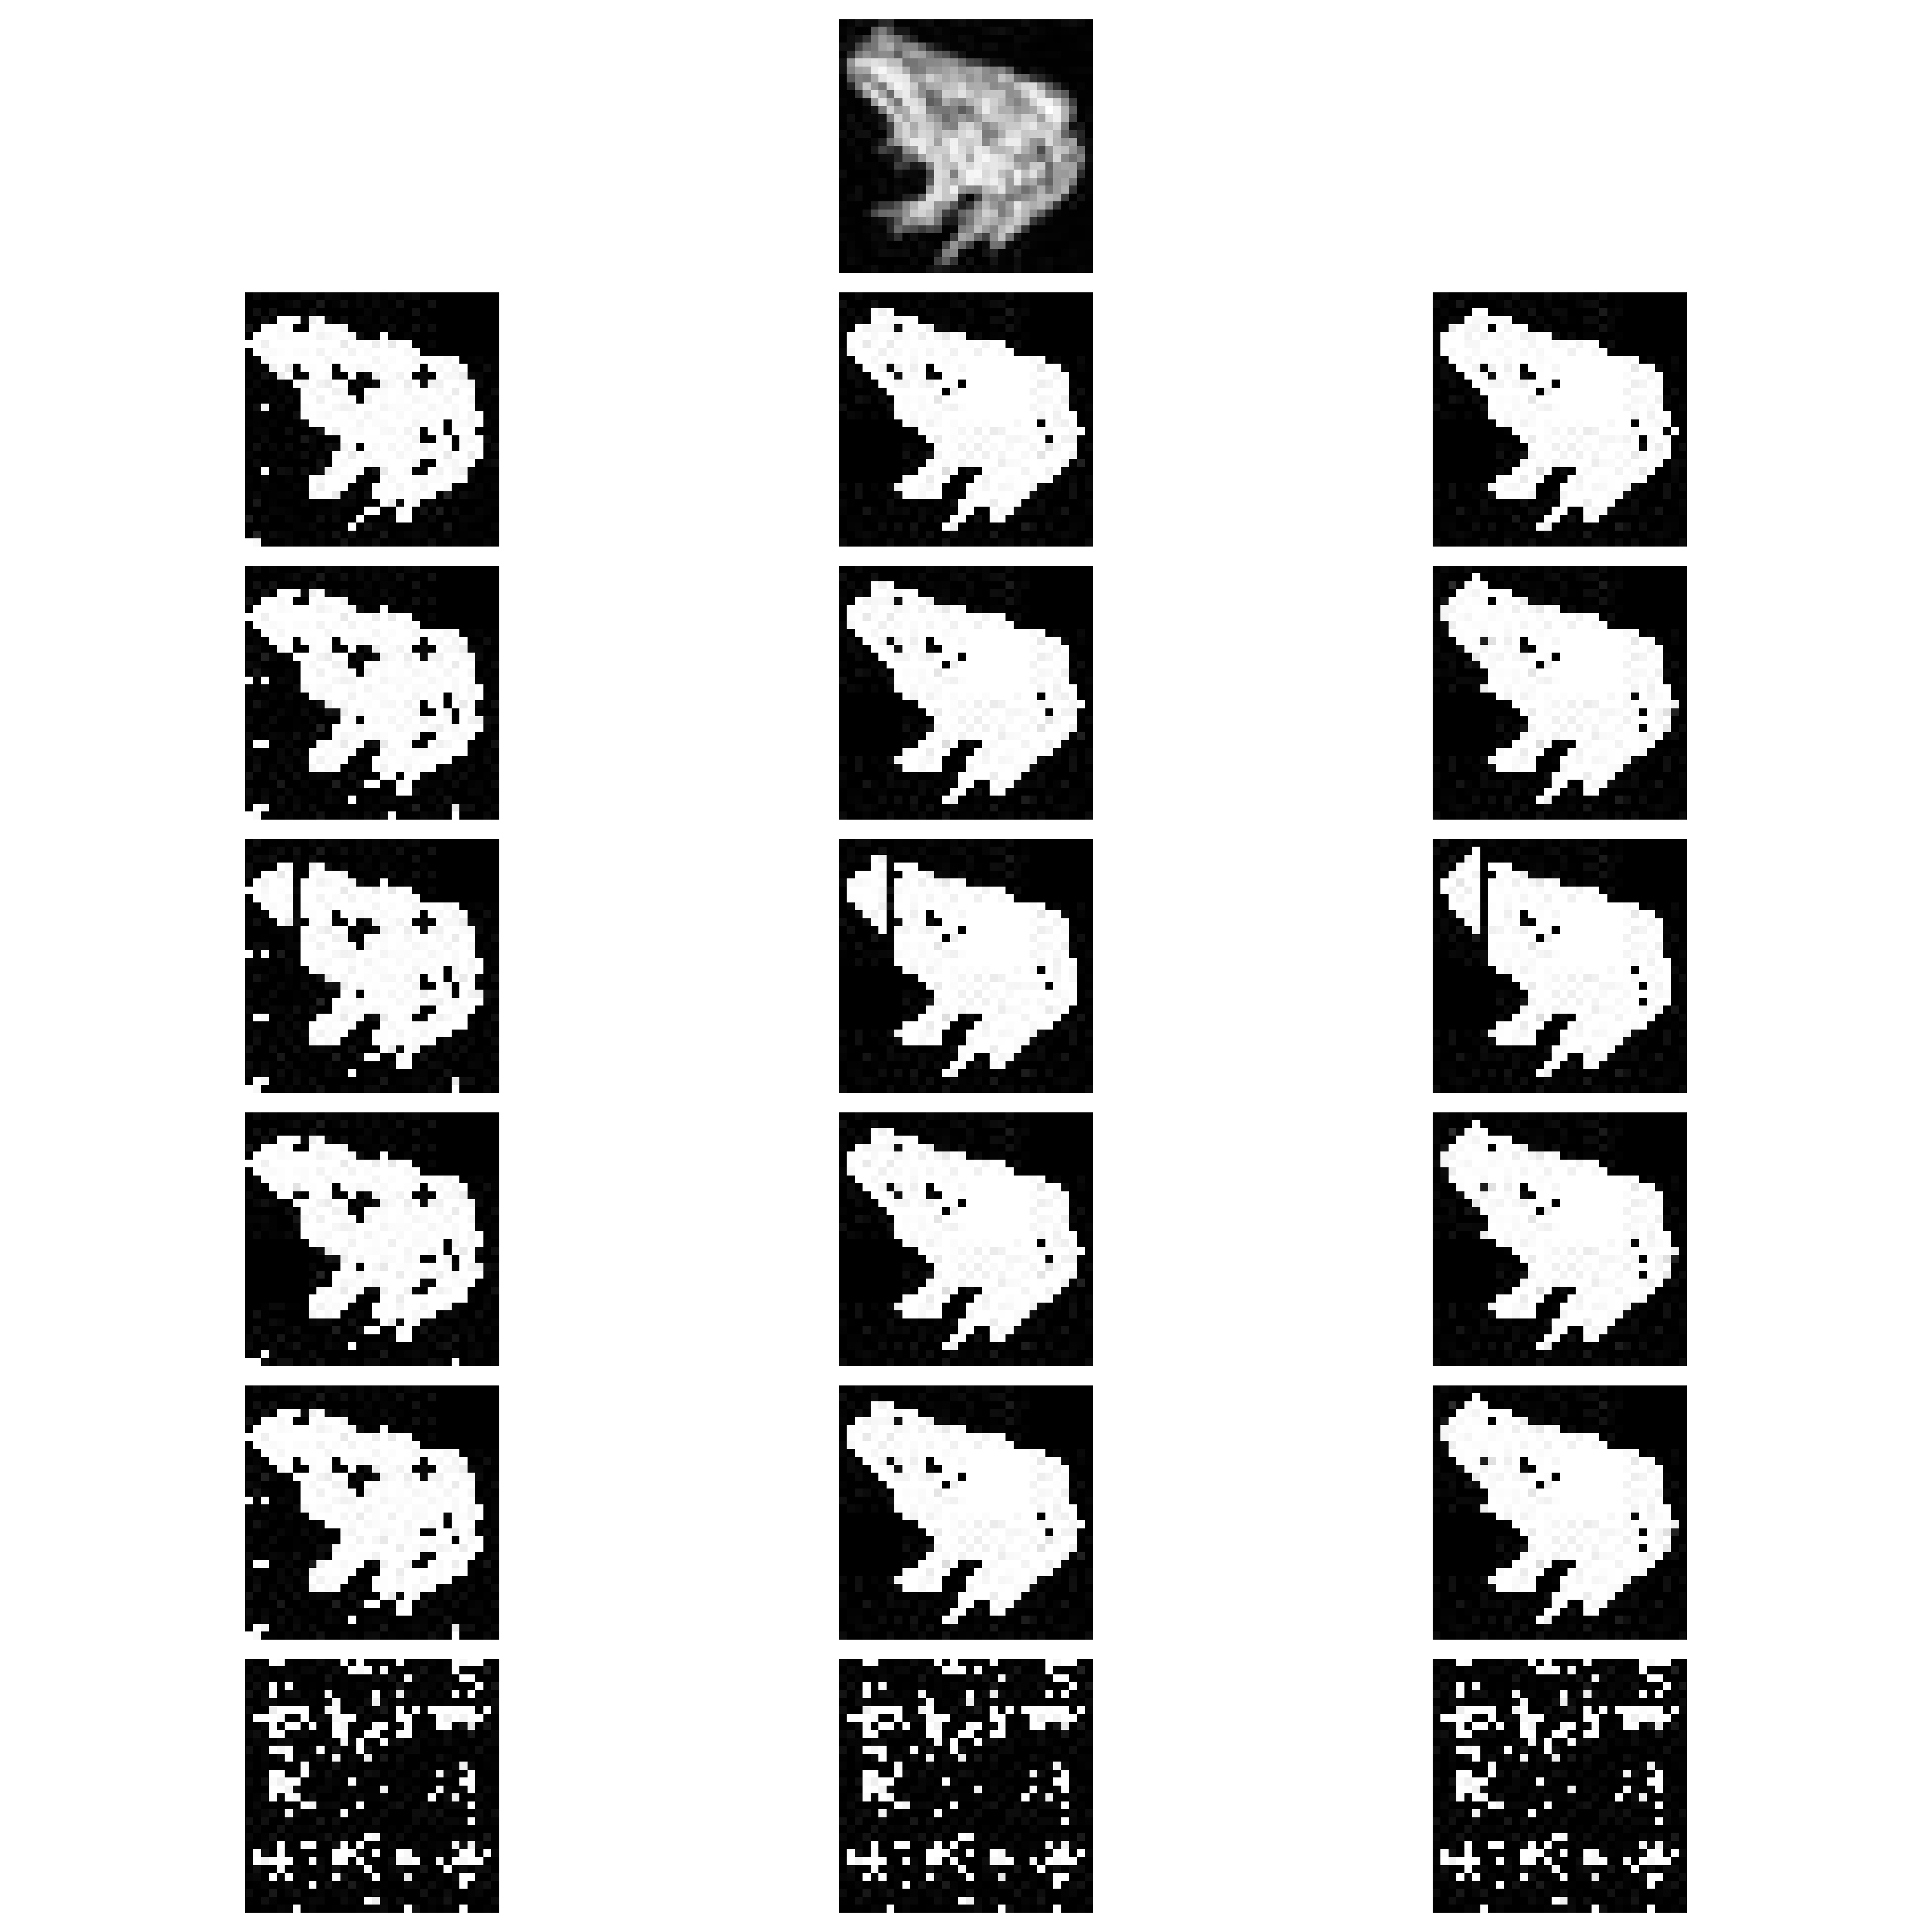
\includegraphics[width=1\linewidth]{Figure/Results/10_24_sample_images.png}
%  \caption{Segmentation  CIFAR-10. $1^{st}$ row input image, $2^{nd}$ row Chan-Vese, $3^{rd}$ row CESN ,  $4^{th}$ row CLSTM, $5^{th}$ row CGRU, $6^{th}$ row CRNN and  $7^{th}$ row 3DCNN at  \textit{1th, 10th and 50th} iteration, respectively.}
%  \label{fig:sample_results_cifar10}
% \end{figure}


\subsubsection{Conclusion}



The CLSTM outperforms the 3DCNN, CGRU and CRNN. The additional data samples improved the CGRU, 3DCNN, CLSTM and CRNN segmentation resutls when compared to the previous two experiment in Section~\ref{sec:BSD} and ~\ref{sec:Weizmann}. The significant increase in the data, resulted in a exponentially improvement in the performance if the CRNN, however, the CESN displayed characteristics of overfitting.  This observation is due to the echo state property mentioned in Section~\ref{sec:echo_state_property_and_spectral_radius} not being satisfied. The CESN although is a efficient alternative to training RNNs, however, optimal performance is not guaranteed due to the number of hyperprameters that need to be optimized and therefore does not perform better than state-of-the-art RNNs under the conditions of this experiment.

\newpage



% ========================================================================= %
% ========================================================================= %

\subsection{CIFAR-100}
\label{sec:cifar_100}

\subsubsection{Introduction}

In this experiment we used the CIFAR-100 database, this database is much more complex that the previous databases due to the additional number classes and significantly larger sample than the BSD and WSD.

\subsubsection{Result And Discussion}

 Table~\ref{table:cifar_100_hyperparameter} shows the optimal parameters for each model selected based on the performance of the models~\footnote{CESN, CRNN, CLSTM, CGRU and 3DCNN are all referred as \textbf{models} for brevity.} on the validation set. The input images are resized to 64$\times$64, therefore, the number of fully-connected units in and hidden units for the CESN, CRNN, CLSTM, CGRU and 3DCNN is 4096, and the optimal leaking rate, spectral radius, sparsity and input scaling for CESN are 0.01, 0.7, 0.2 and 1, respectively. The optimal parameters are chosen by maximizing the IoU on the validation set.
\begin{table}[H]
    \centering
        \caption{CIFAR-100 dataset optimal parameters for the CESN, CRNN, CLSTM, CGRU and 3DCNN}
    \resizebox{\linewidth}{!}{
    \begin{tabular}{ccccccc}
    \hline
    \textbf{Model} &  \textbf{Hidden size} & \textbf{Leaking rate} & \textbf{Sparsity} & \textbf{Spectral radius} & \textbf{Input scaling}\\
    \hline
      CESN   & 4096   & 0.0713  & 0.2  &  0.9  & 1.0  \\
      CRNN   & 4096   & -  & -  &  -  & -   \\
      CLSTM  & 4096   &    & -  &  -  & -    \\
      CGRU   & 4096   & -  & -  &  -  & -     \\
      3DCNN   & 4096   & -  & -  &  -  & -     \\
    \hline
    \end{tabular}}
    \label{table:cifar_100_hyperparameter}
\end{table}

Figure~\ref{fig:cifar_100_model_loss} shows the training and validation loss of the CESN, CRNN, CLSTM, CGRU and 3DCNN versus the number of epochs (i.e. data passes). The training and validation loss are decreasing with further training, and since the validation loss is slightly greater than training loss, this means that the models are able to generalise on unseen observation and mostly likely to not overfit on the training set, the reasons are twofold, 1) decaying learning rate which helps the models converge to local minima and avoid oscillations~\cite{you2019does}, 2) dropout connection with a probability of 50\% between the convolutional layers help with overfitting, especially when working deep learning models that have large number of parameters as the one considered in this study~\cite{hinton2012improving} 3) training with more data.


All the models the loss is decreasing with some observer exception especially for CRNN, this is a direct indications of the ability of the models to learn the LS function, the CGRU has the lowest validation loss, followed by, CLSTM, 3DCNN, CESN and lastly the CRNN. The CRNN in the early stages (i.e. $\approx$ 100 epochs)of training the loss in increasing, this mostly likely due the vanishing and exploding gradients~\cite{pascanu2013difficulty} mentioned in Section~\ref{sec:Recurrent_Neural_Networks}. And CGRU and 3DCNN validation loss curves are very close to each other, and exhibit similar trend, which means they are more likely to have the similar performance. These curves are used to monitor overfitting and underfitting during training, however, since we implemented early stopping to stop the training when overfitting occurs.

% Figure~\ref{fig:cifar_100_model_loss} shows the training and validation loss of the CESN, CRNN, CLSTM, CGRU and 3DCNN against the number of epochs. The training and validation loss are decreasing with further training, this means that the models are not overfitting on the training set, and for all the models the loss is decreasing with different magnitude, this is a direct indications of the ability of the models to learn the LS function, the CGRU has the lowest validation loss, followed by, CLSTM, 3DCNN, CRNN and lastly the CESN. The CESN has the lowest starting loss, however a lower rate of change in loss compared to CRNN, CLSTM, CGRU and 3DCNN. And CLSTM, CGRU, CRNN and 3DCNN loss curves are close to each other, and exhibit similar trend, which means they are more likely to have the similar performance.

\begin{figure}[H]
\centering
  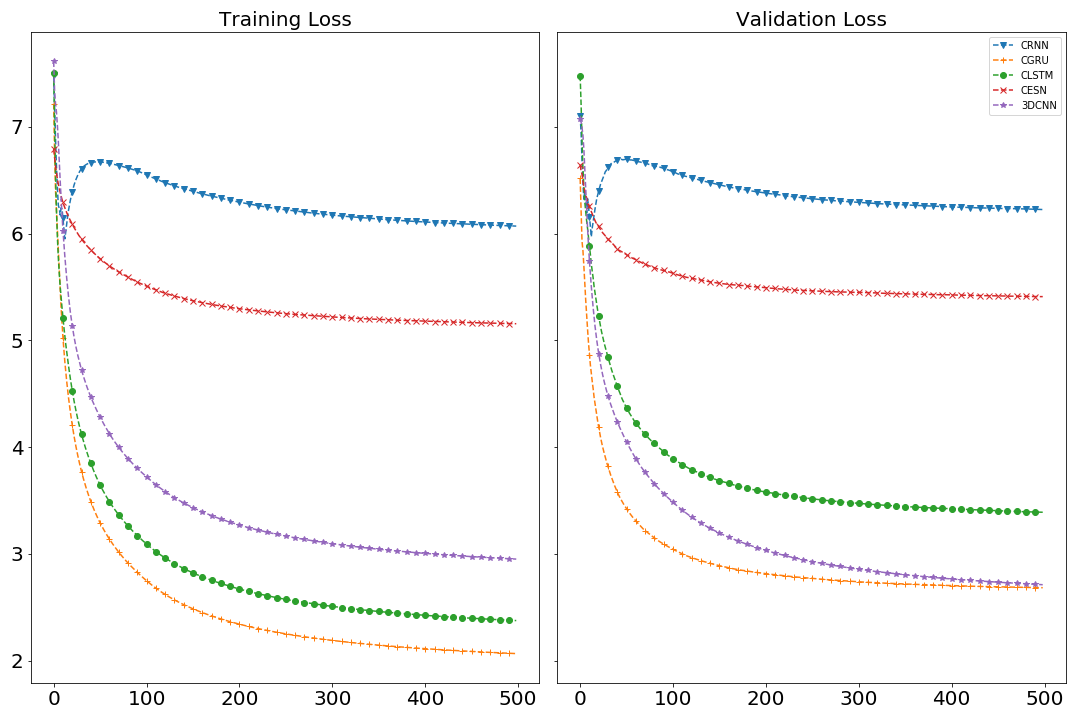
\includegraphics[width=1\textwidth]{Figure/Results/CIFAR_100_loss.png}
\caption{CIFAR-100 validation dataset learning curves for the CESN, CLSTM, CGRU, RNN and 3DCNN}
 \label{fig:cifar_100_model_loss}
\end{figure}

Figure~\ref{fig:cifar_10_model_perfomance} shows the precision, recall, $F_{1}Score$ and IoU of the CESN, CRNN, CLSTM, CGRU and 3DCNN on the validation set. The CESN, CLSTM, CGRU and 3DCNN start with a lower performance with a single pass of the data, with further training the models performance increases and until it becomes constant at which further training does not make performance better or worse, this can be attributed a small learning rate as a result of the decaying rate. The CRNN performance drop with further training, this phenomenon is due to the the high rate rate, which causes the network to become unstable and results in vanishing and exploding gradients~\cite{pascanu2013difficulty}. The decaying learning rate procedure resolves the vanishing and exploding gradients of the CRNN as a stable increase in the precision, recall, $F_{1}Score$ and IoU~\cite{you2019does}.

In Figure~\ref{fig:cifar_10_model_perfomance}, the precision is slightly higher than the recall for all the models, this implies that the models slightly more sensitive to undersegmentation than oversegmentation~\cite{sigut2015over, troya2015unsupervised}, the latter can be due to the proportion of noise introduced by up-resizing the images. The CGRU has the highest precision and recall, followed by, 3DCNN, CLSTM, CESN and lastly CRNN the  throughout the entire training process. The most interesting observation, is the CGRU, CLSTM, CRNN and 3DCNN converge towards a single recall and precision, this is not surprising, since these models require large amounts of data in order to achieve state-of-the-art results.

The $F_{1}Score$ is higher than the IoU in Figure~\ref{fig:cifar_10_model_perfomance}, this is because the models are penalized more for incorrectly classified segmentations boundaries. The CRNN have the lowest IoU and $F_{1}Score$, this is due to the unstable gradients during back-propagation~\cite{pascanu2013difficulty}. While the, CLSTM, CGRU and 3DCNN are able to capture both the spatial-temporal evolution of the LS, therefore LS foreground pixels from earlier time step are now seen as noise, this is due to the ability of the CLSTM, CGRU and 3DCNN to capture the short-term and long-term memory, therefore having a global spatial-temporal view of the LS evolution. The CESN is performing better than CRNN, and this advantages is due the de-coupling of the sparse reservoir and readout layer during training and as such does not suffer from the vanishing and exploding gradients~\cite{jaeger2001echo,jaeger2002tutorial,lukovsevivcius2009reservoir}.


% Figure~\ref{fig:cifar_100_model_perfomance} shows the precision, recall, $F_{1}Score$ and IoU of the CESN, CRNN, CLSTM, CGRU and 3DCNN on the validation set. All the models start with a lower performance with a single pass of the data, with further training the models performance increases and until it becomes constant at which further training does not make performance better or worse, this is mostly due to the a small learning rate or size of the training data.

% Lets look at the precision and recall curves, the precision is sightly higher than the recall for all the models, this means that the models are more likely to under-segment than over-segment the image, therefore the models ability to capture finer changes of the LS such that they are different from the noise is challenging. The CGRU has the highest precision and recall, followed by, CLSTM, CRNN, 3DCNN and lastly the CESN throughout the entire training process. The most interesting observation, is the CGRU, CLSTM, CRNN and  3DCNN converge towards a single recall and precision, this is not surprising, since these model require large amounts of data in order to achieve state of the art results. The number of parameters of the CESN make it difficult to find the optimal parameters such the echo state property is satisfied, which then lead to sub-optimal performance.

% Now lets look at the $F_{1}Score$ and IoU, clearly the modes are slightly penalized more for incorrect classified segmentation, this is seen from $\approx$ 5\% higher $F_{1}Score$ than IoU. The CGRU has the highest $F_{1}Score$ has the highest  followed by, CLSTM, 3DCNN, CRNN and lastly the CESN, but, when is comes to IoU 3DCNN is better than CLSTM, this might be related to boundaries of the segmentation not clearly defined compare to the 3DCNN. The ESN has the worst IoU and $F_{1}Score$, this is because the CESN is more sensitive to the noise and therefore unable to capture the spatial evolution of the LS, while the other CRNN, CLSTM, CGRU and 3DCNN are able to capture both the spatial and temporal evolution of the LS.


\begin{figure}[H]
\centering
  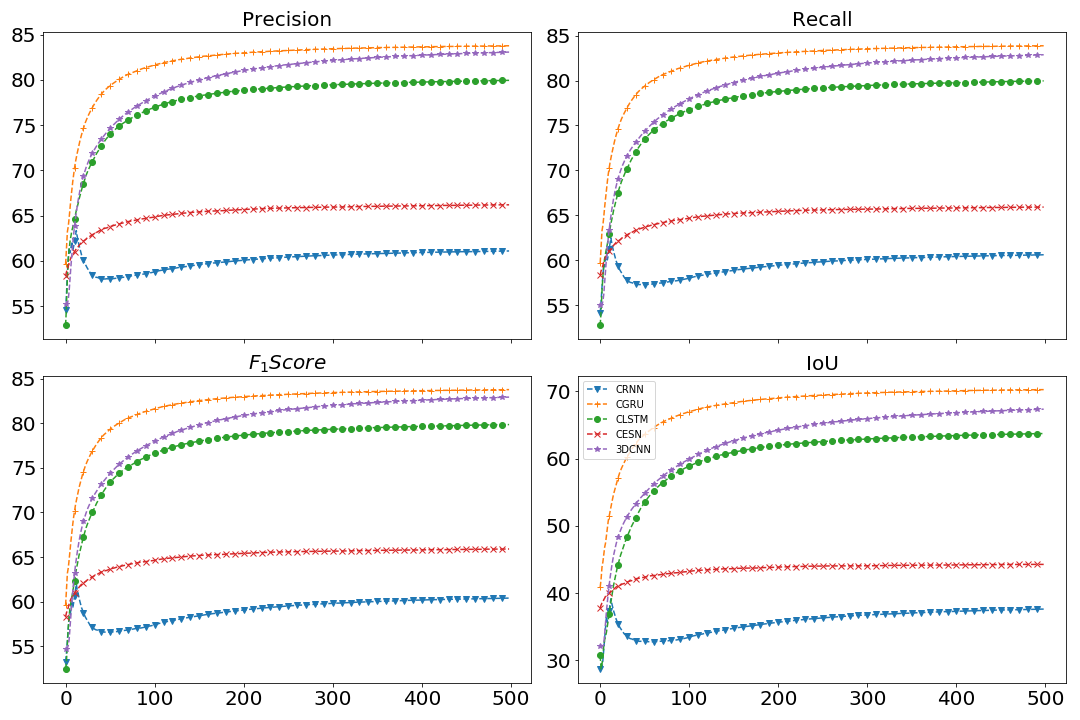
\includegraphics[width=1\textwidth]{Figure/Results/CIFAR_100_performance.png}
\caption{CIFAR-100 validation dataset learning curves for the CESN, CLSTM, CGRU, RNN and 3DCNN}
 \label{fig:cifar_100_model_perfomance}
\end{figure}


Table~\ref{tab:cifar_100} shows the performance of the CESN, CRNN, CLSTM, CGRU and 3DCNN on the testing set. In addition, white noise is measured in order to determine the proportion of pixels that are considered to be random noise in the testing set, about 50\% of the the foreground pixels are noise as seen from the recall. Basically, this means the predictability of our models is benchmarked between being able to learn the spatio-temporal evolution of the LS or being a sequence of random numbers, therefore, cannot be predicted.  

The CESN is performing better than random with a IoU of 44.5\%. The CGRU with a IoU of 71.5\% outperforms all the other models, followed by, the 3DCNN with a IoU of 69.4\%, CLSTM with a IoU of 65.3\% and CRNN with a IoU of 48.7\% . Even with a significant increase in data the CESN is still unable capture the spatio-temporal evolution of the LS as compare to the CGRU, CLSTM, CRNN and 3DCNN, due to overfitting  because of it's short-term memory, such that, for short-term memory the LS pixels are have similar characteristics to random noise, since the final segmentation state of the LS is dependent on both the information of the initial states and the current state of the LS, therefore, model which are able to capture both long-term and short-term memory have a advantage. 

% Table~\ref{tab:cifar_100} shows the of the CESN, CRNN, CLSTM, CGRU and 3DCNN on the testing set. In addition, we added random noise to measure the proportion of noise in the testing set, about 50\% of the the foreground pixels are noise as seen from the recall. The CESN is performing better than random noise with IoU of 44.5\%, and the CRNN with a IoU of 48.7\%. The top three performing model are CGRU IoU of 71.5\%, 3DCNN IoU of 69.4\% and CLSTM IoU of 65.3\%. On the testing set we can see that recall is larger than the precision, which means the models are over-segmenting the images, this may be due to over-fitting or the upsampling $32\times32 \rightarrow 64\times64$ of the images which may introduced artifacts not part of the LS evolution.


\begin{table}[H]
 \centering
 \caption{CIFAR-100 testing results. Here we compare various models and noise is also included.}
\resizebox{\linewidth}{!}{
    \begin{tabular}{cccccc}
    \hline
    \textbf{Method} & \textbf{IoU} &  \textbf{Precision} &  \textbf{Recall} & \textbf{$F_{1}Score$}    \\
    \hline
CGRU 	&	\textbf{71.5}\% &	\textbf{84.2}\% &	\textbf{85}.0\% &	\textbf{83.9}\%\\
3DCNN 	 &	69.4\% &	82.8\% &	84.0\% &	82.6\%\\
CLSTM 	 &	65.3\% &	79.9\% &	81.8\% &	79.8\%\\
CRNN 	 &	48.7\% &	68.0\% &	69.3\% &	69.7\%\\
CESN 	 &	44.5\% &	64.8\% &	65.4\% &	66.0\%\\
White Noise   & 30.2\%    & 50.0\%      & 50.0\%    & 49.5\%  \\
    	\hline
    \end{tabular}}
    \label{tab:cifar_100}
\end{table}

Figure~\ref{fig:sample_results_cifar100} shows samples segmentation the 1$^{st}$, 2$^{nd}$, 3$^{rd}$, 4$^{th}$, 5$^{th}$, 6$^{th}$ and 7$^{th}$ columns are the input images, ground-truth (i.e. LS), CESN, CRNN, CLSTM, CGRU and 3DCNN, respectively. We observe that CESN is able to capture spatial properter of the LS segmentation, however, but seems to be struggling to capture the temporal evolution this is seen by the checkerbox structures in Figure~\ref{fig:sample_results_cifar100}, since the LS is initialized as checkerbox. 

The CRNN, CLSTM , CGRU and 3DCNN are able to capture the boundaries especially non-overlapping objects, but due to over-segmentation as seen from a larger recall than precision in Table~\ref{tab:bsd500}, the boundaries are not well-defined, this could be due to that the training was stopped prematurely.

% Figure~\ref{fig:sample_results_cifar100} shows samples segmentation, first, second, third, fourth, fifth, sixth and seventh columns are the input images, ground-truth (i.e. LS), CESN, CRNN, CLSTM, CGRU and 3DCNN, respectively. The CESN is unable to capture the time evolution of the LS, this seen from the cheakerbox like structures, which are present in the earlier time steps of the LS. The CRNN, CLSTM, 3DCNN and CGRU are able to capture the boundaries for non overlapping objects, however, suffer from over-segmentation, and they are able to segment, and the segmentation boundaries are over-segmented. The CRNN, CLSTM, CGRU as seen in the images are able to capture the temporal evolution of the LS.

\begin{figure}[H]
\centering
  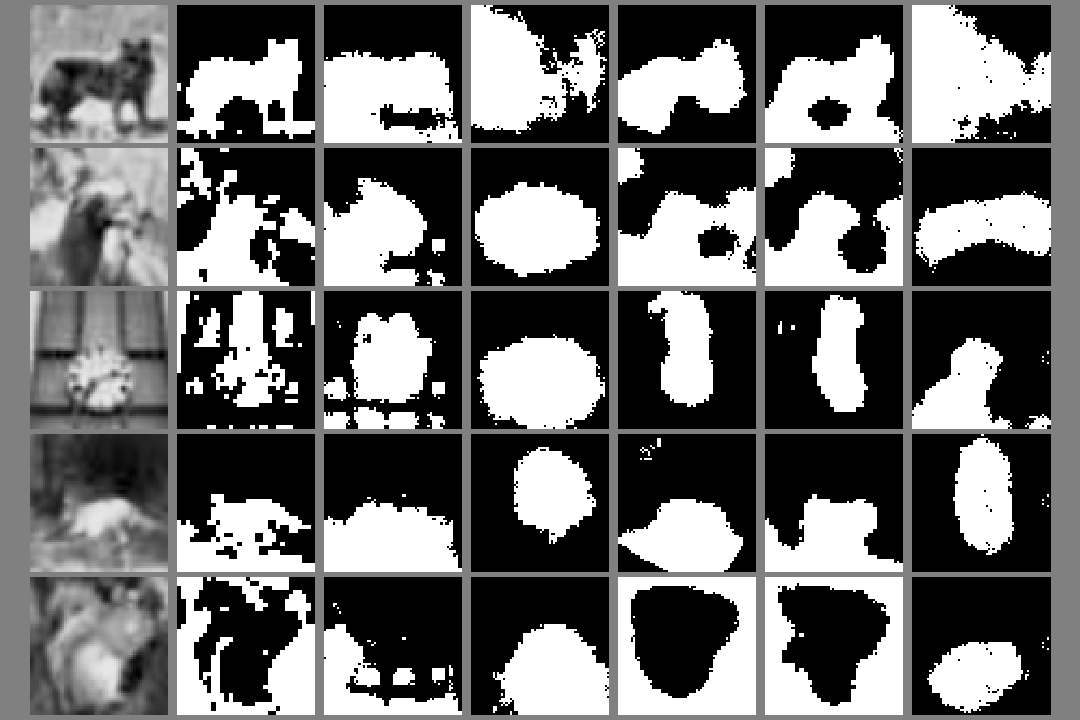
\includegraphics[width=1\linewidth]{Figure/Results/CIFAR_100_sample.png}
 \caption{CIFAR-100 examples of iterative segmentation. $1^{st}$ column input, $2^{nd}$ Chan-Vese, $3^{rd}$ column CESN, $4^{th}$ CRNN, $5^{th}$ column CLSTM , $6^{th}$ column CGRU , $7^{th}$ column 3DCNN.}
 \label{fig:sample_results_cifar100}
\end{figure}

% \begin{figure}[H]
% \centering
%   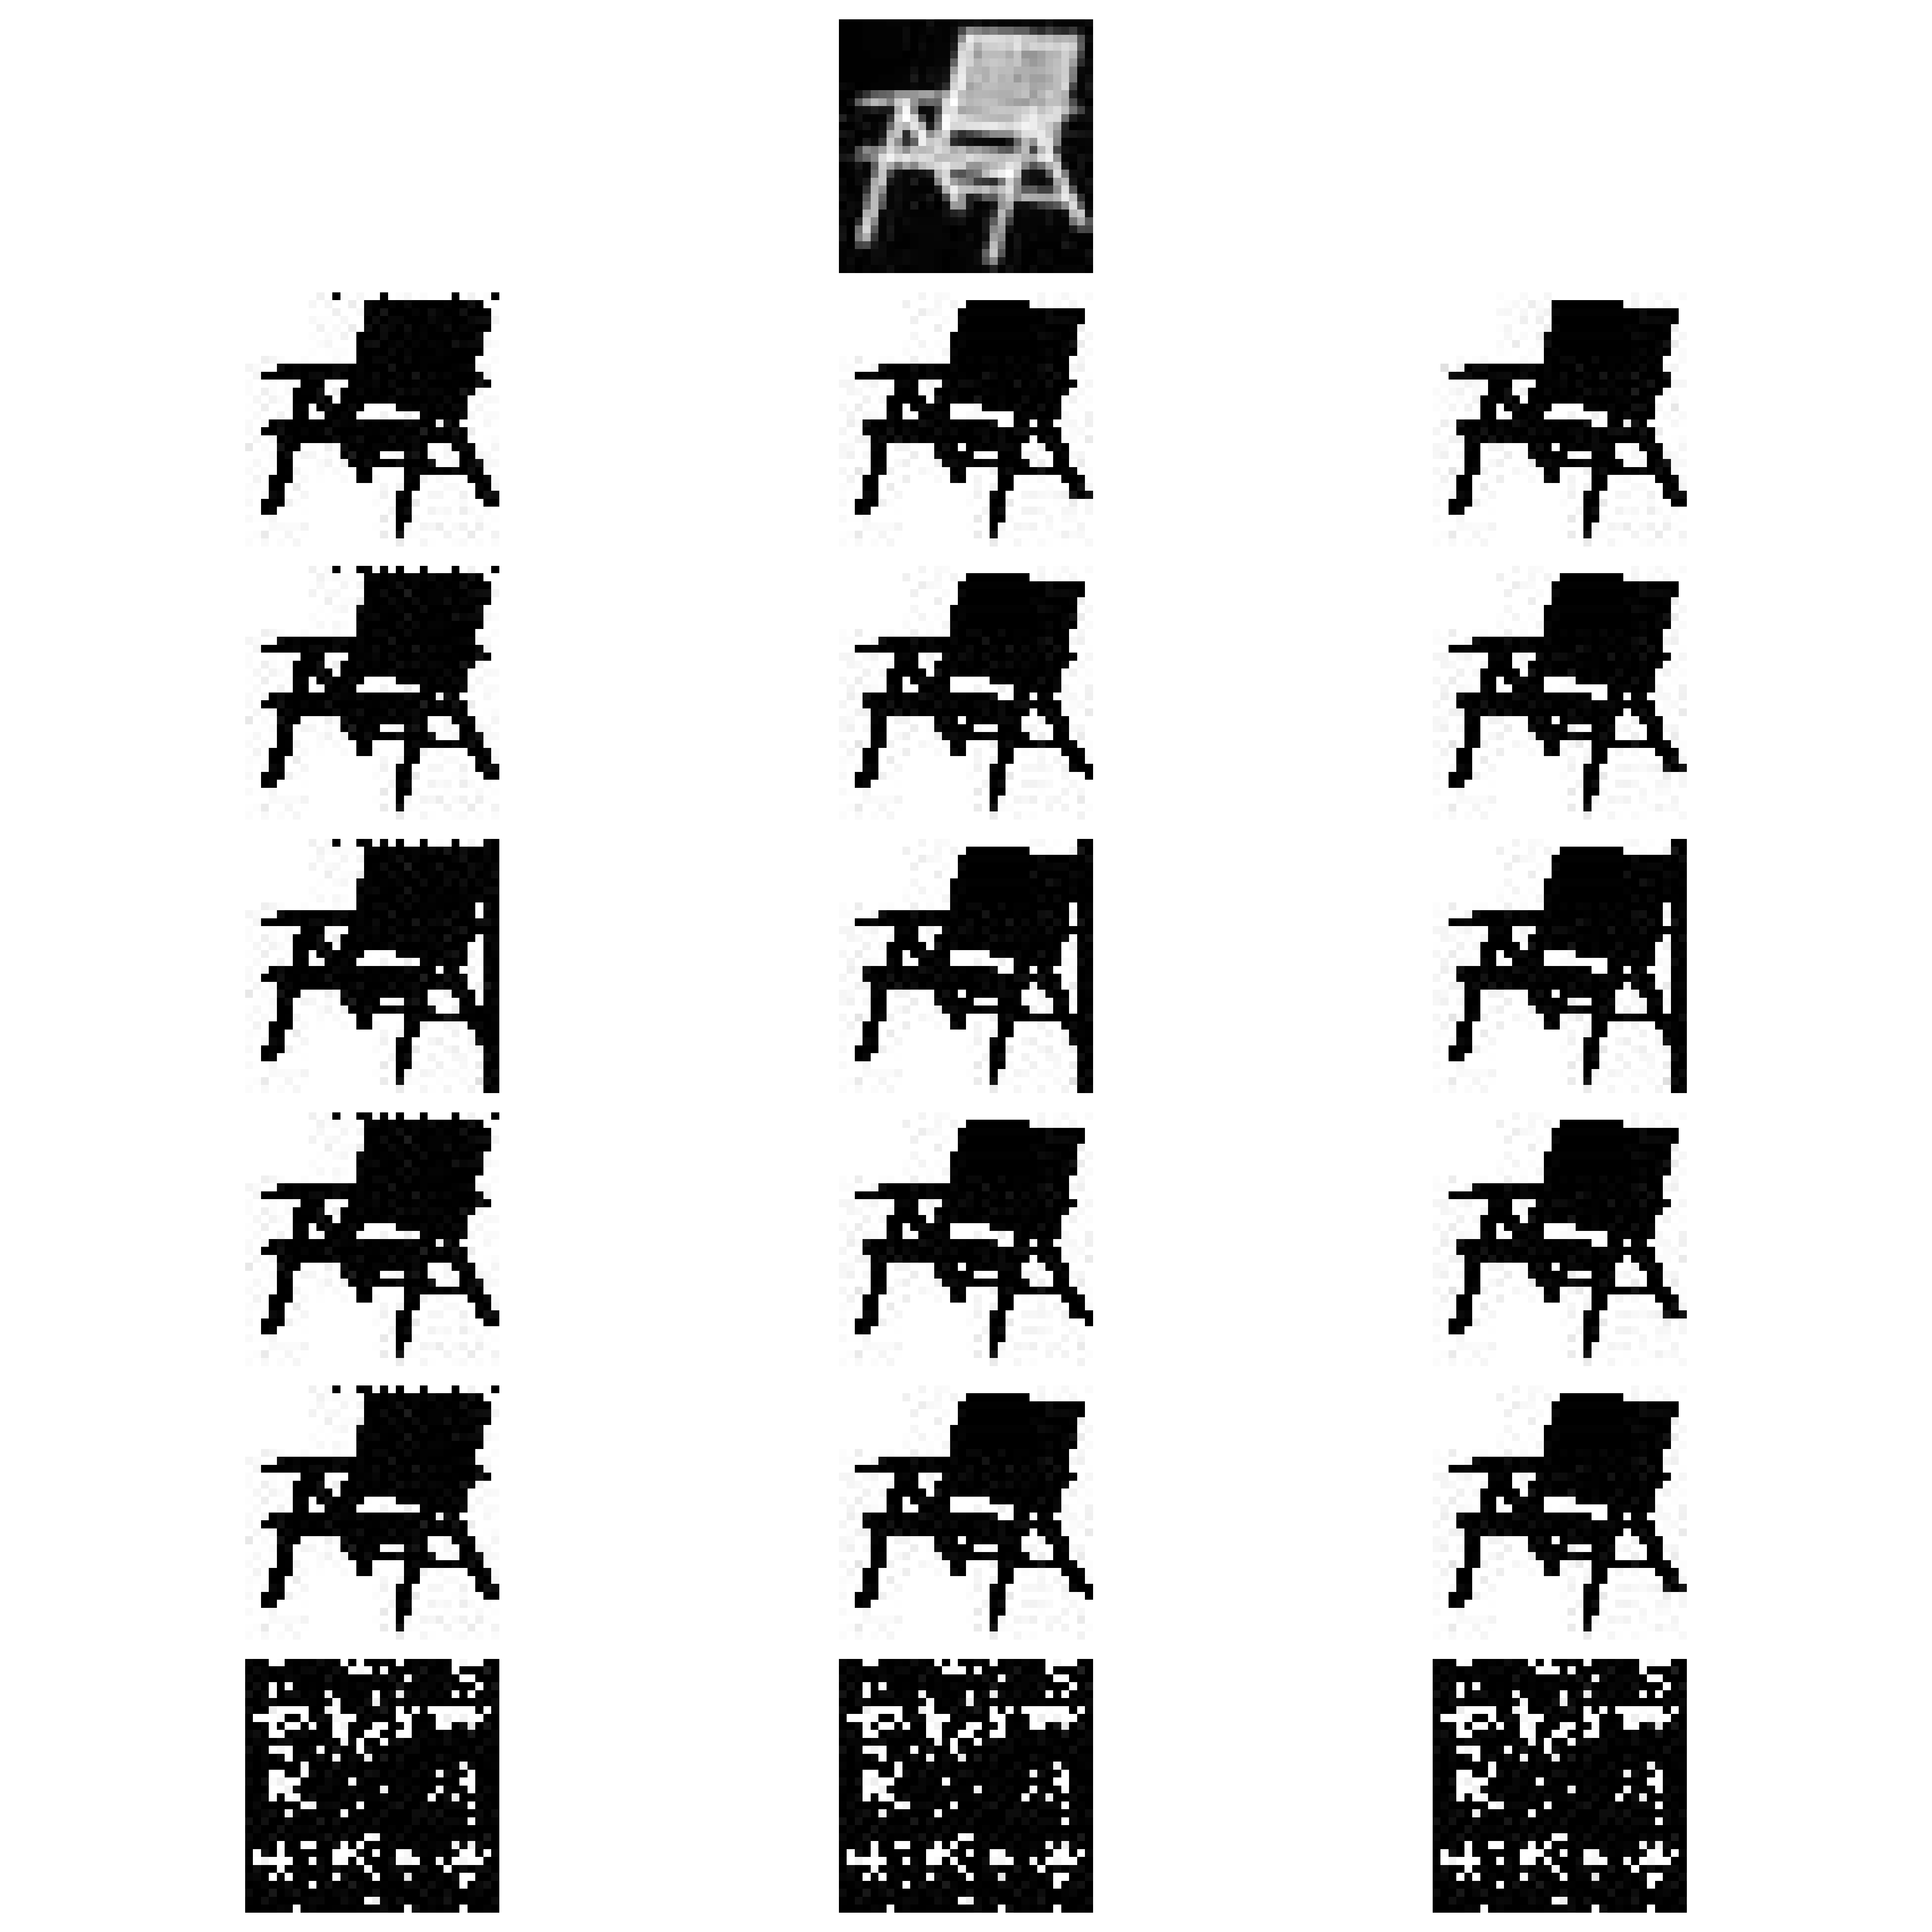
\includegraphics[width=1\linewidth]{Figure/Results/100_383_sample_images.png}
%  \caption{CIFAR-100 examples of iterative segmentation. $1^{st}$ column input, $2^{nd}$ Chan-Vese, $3^{rd}$ column CESN, $4^{th}$ CRNN, $5^{th}$ column CLSTM , $6^{th}$ column CGRU , $7^{th}$ column 3DCNN.}
%  \label{fig:sample_results_cifar100}
% \end{figure}


\subsubsection{Conclusion}
 
 The CGRU outperforms the 3DCNN, CLSTM and CRNN. The additional data samples improved the CGRU, 3DCNN, CLSTM and CESN segmentation resutls when compared to the previous two experiment in Section~\ref{sec:BSD} and ~\ref{sec:Weizmann}. In twist of events, the CESN performed better than the CRNN on the validation than testing set. The CESN segmentation results are better in comparison to all the previous experiments, although not optimal, this validates that the reservoir is task specific and requires domain expertise to find optimal parameters~\cite{jaeger2002tutorial,lukovsevivcius2009reservoir}. The CESN although is a efficient alternative to training RNNs, however, optimal performance is not guaranteed due to the number of hyperprameters that need to be optimized and therefore does perform better than state-of-the-art RNNs under the conditions of this experiment.

\subsection{Reservoir Dynamics}
\label{sec:reservoir_dynamics}

\subsubsection{Introduction}

In order to successfully model a task using ESN, it crucial to understand the dynamics of the reservoir. As recommended in Jaeger et al (2003) ~\citep{jaeger2002tutorial}, that one should plot the internal dynamics if they want to understand the learning processes in ESN. The performance of the reservoir is highly dependent on the setting of the parameters discussed in detail in Section~\ref{sec:Dynamics_and_reservoir_characteristic}, for tasks that are non-linear the reservoir has to be also non-linear, and if the task requires to long-term or short-term memory the reservoir should be set a such. 
\subsubsection{Results And Discussion}

In Figure~\ref{fig:input_activity}, ~\ref{fig:reservoir_activity} and ~\ref{fig:readout_activity} we inspect the internal dynamics of ${\mathbf{\Theta}}^{in}$, ${\mathbf{\Theta}}$ and ${\mathbf{\Theta}}^{out}$, the input, reservoir and readout weights for each experiment, respectively. Please note that the figures are centered around zero,  in order to interpret dynamics.



\begin{figure}[H]
\centering
  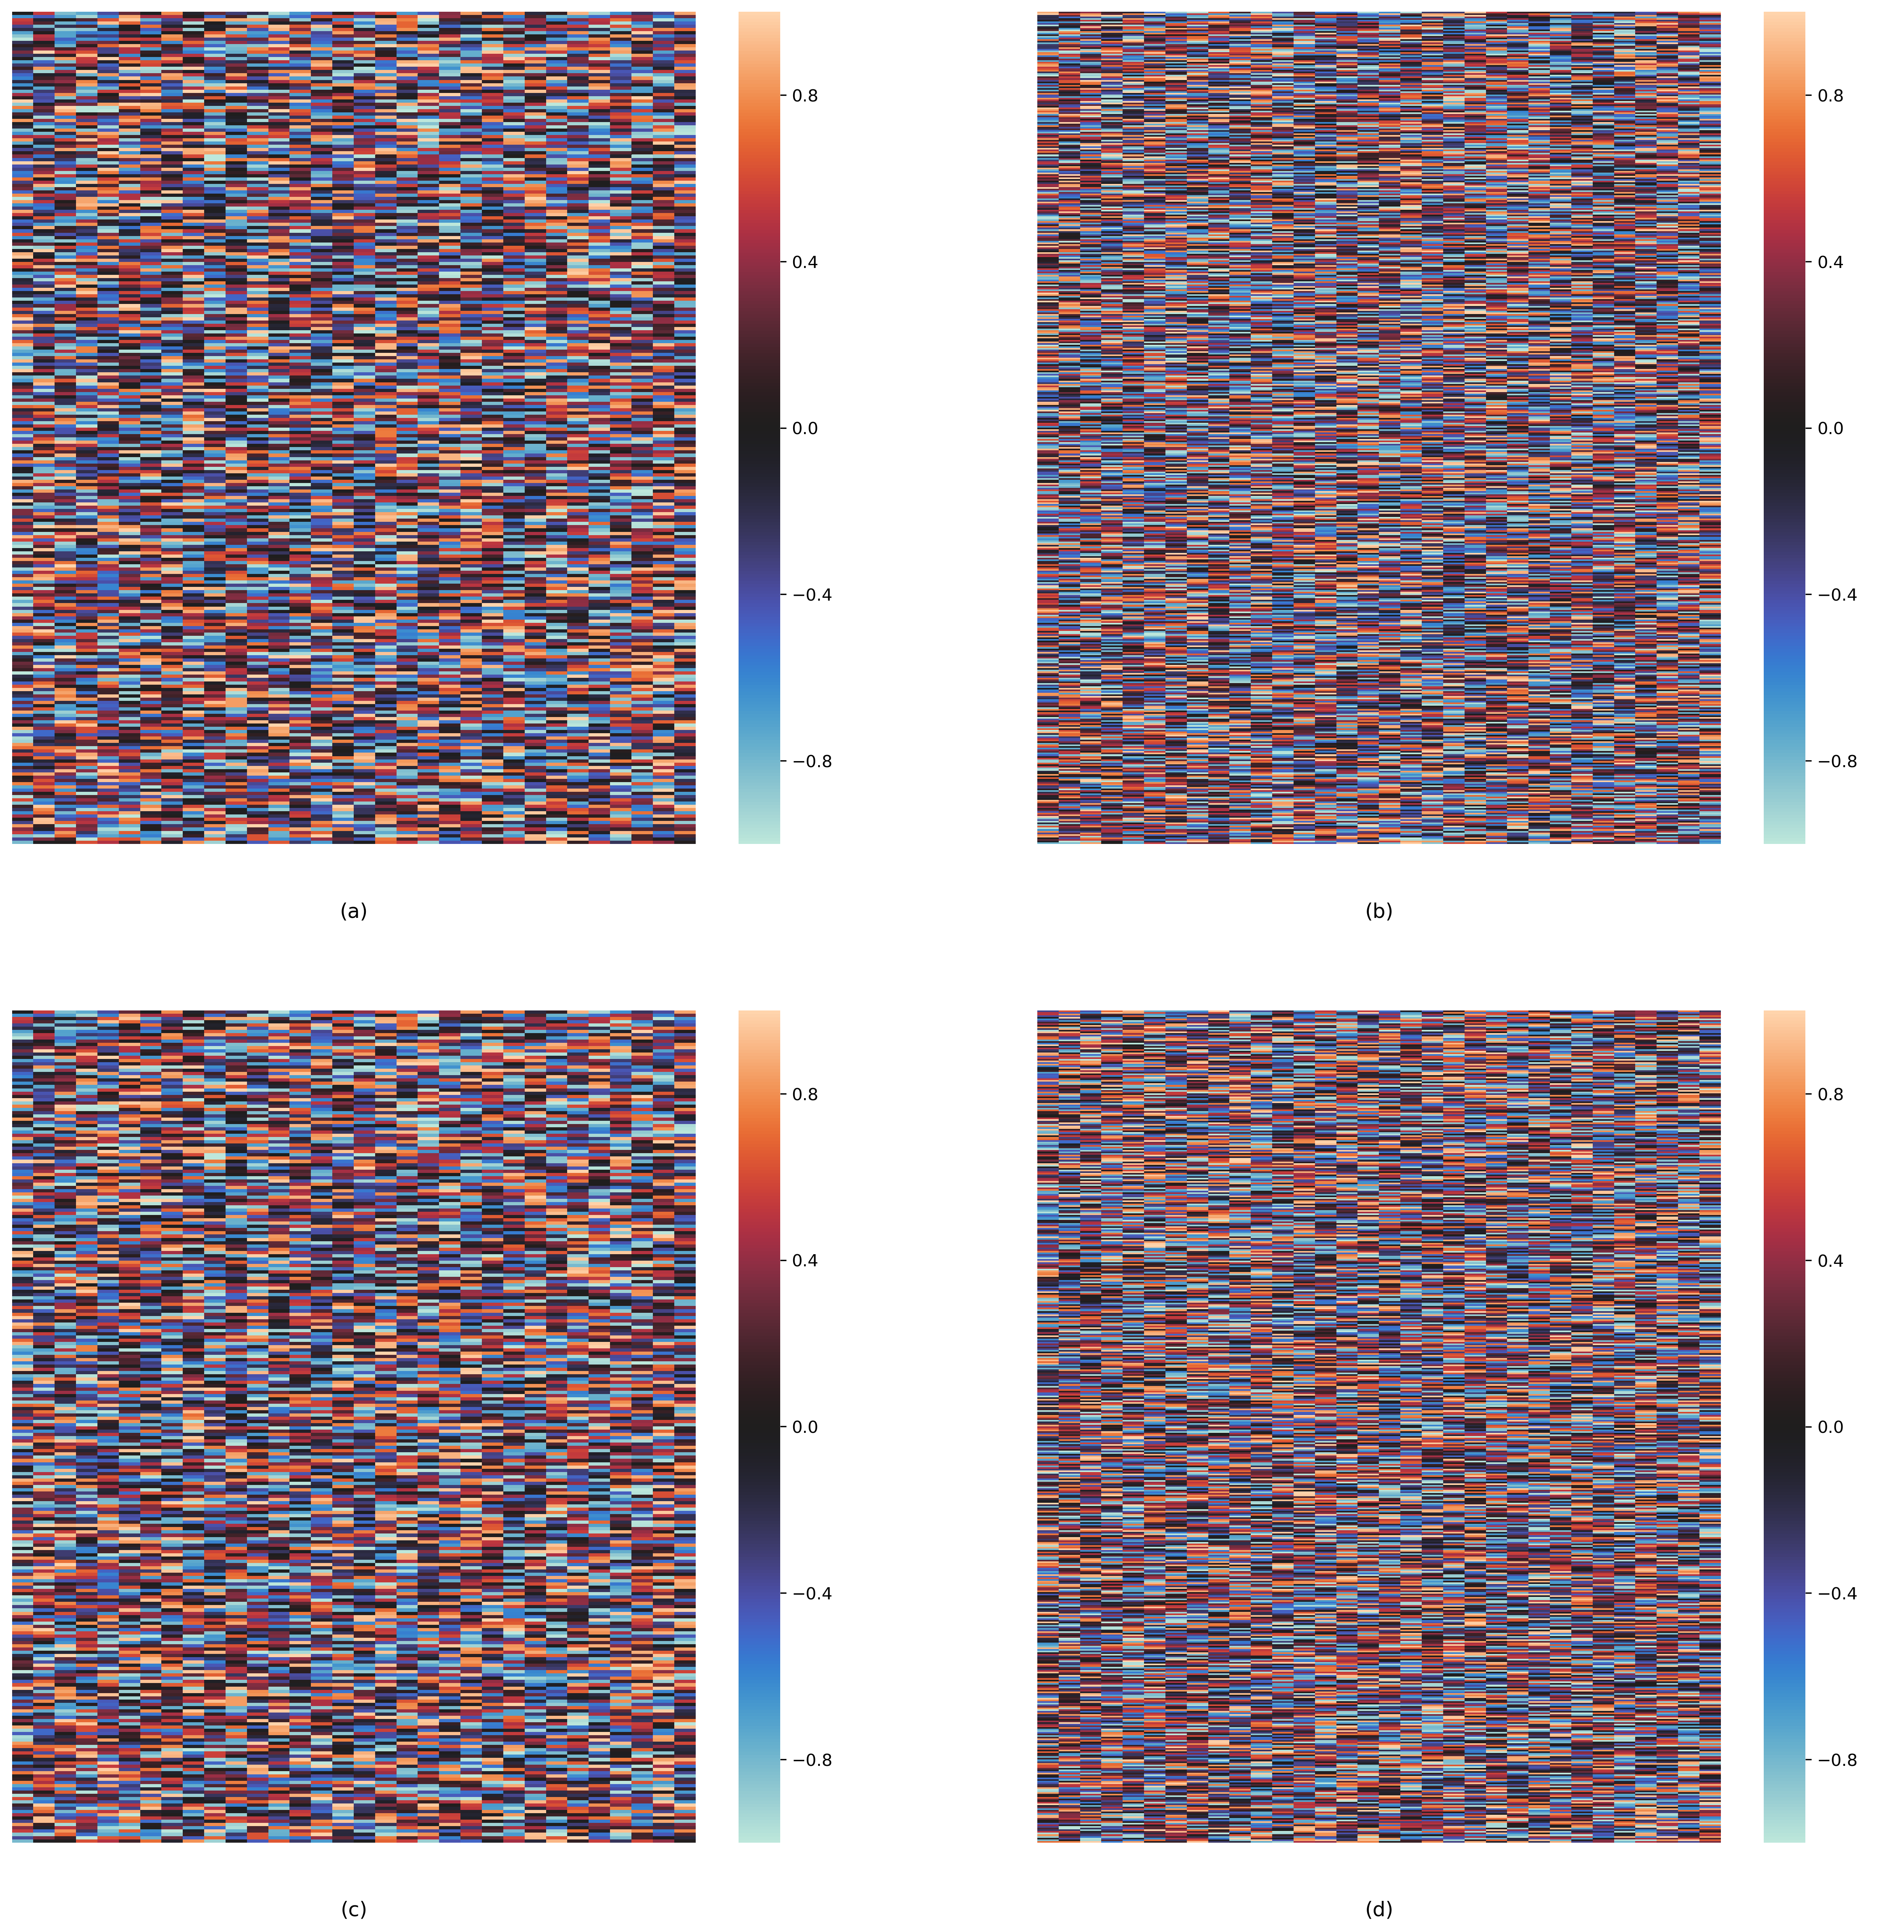
\includegraphics[width=1\textwidth]{Figure/Results/Reservoir_activity_Input_weights_activity_.png}
 \caption{Input weights distribution, a, b, c and d are dynamics of input-reservoir connections for the CIFAR-10, CIFAR-100, BSD and WS dataset.}
 \label{fig:input_activity}
\end{figure}

Even though the inputs weight matrix ${\mathbf{\Theta}}^{in}$ are not trained, their configuration is important. Figure~\ref{fig:input_activity}, shows that the magnitude of the elements in ${\mathbf{\Theta}}^{in}$ are large, which means the reservoir dynamics are strongly driven by the inputs signal $\mathbf{u}(n)$ and also the reservoir neurons operate near the saturation point of $tanh$, this results in nonlinear dynamics of the model. This properties are required to have an excitable reservoir driven by the inputs~\cite{jaeger2007optimization}.


\begin{figure}[H]
\centering
  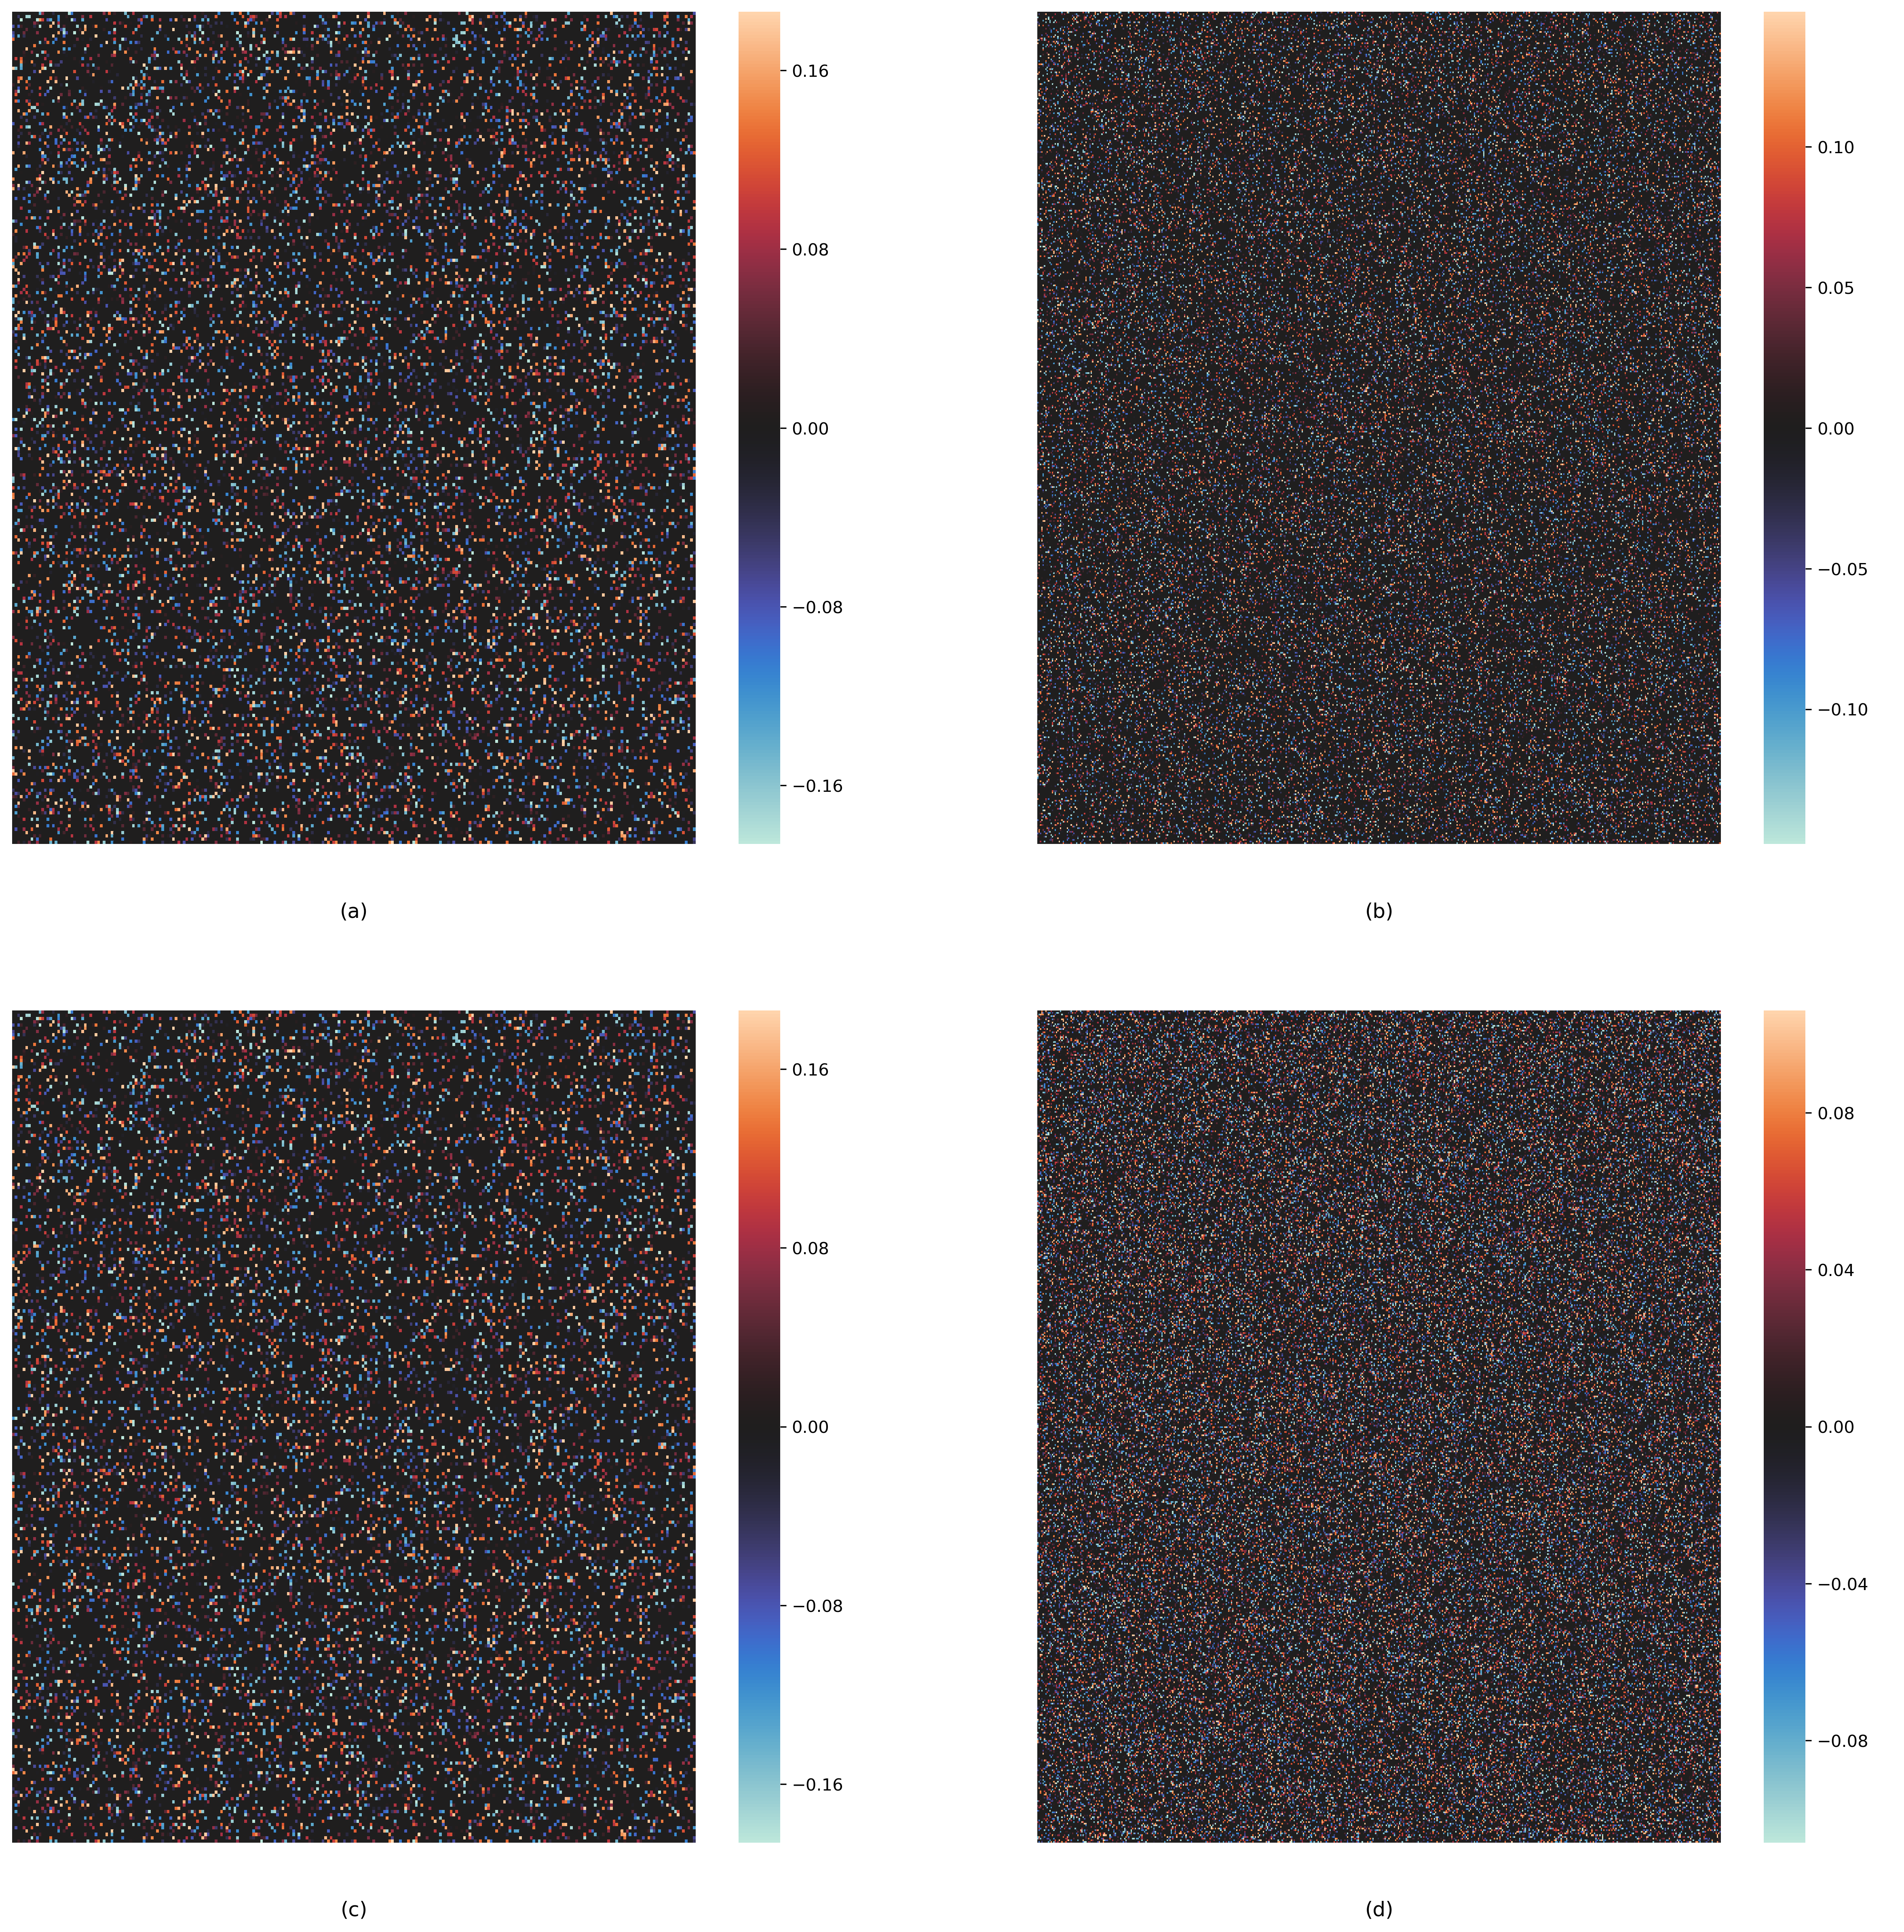
\includegraphics[width=1\textwidth]{Figure/Results/Reservoir_activity_Reservoir_weights_activity_.png}
 \caption{Reservoir weights distribution, a, b, c and d are dynamics of reservoir-reservoir connections for the CIFAR-10, CIFAR-100, BSD and WS dataset.}
 \label{fig:reservoir_activity}
\end{figure}

In Figure~\ref{fig:reservoir_activity}, we have a reservoir with 4096 neurons with a sparsity of 80\%, which mean 20\% of the neurons in  ${\mathbf{\Theta}}$ are non-null elements. The non-null elements are samples from a uniform distribution over [-1,1] and the ${\mathbf{\Theta}}$ was scaled with a spectral radius of 1, 0.9, 0.9 and 0.8 for the Weizamman, BSD, CIFAR-10 and CIFAR-100 experiments respectively, as described in Section~\ref{sec:Dynamics_and_reservoir_characteristic}.  The reservoir dynamics for Weizamman and BSD experiment exhibit similar characteristics even though scaled with different spectral radius, as well as CIFAR-10 and CIFAR-100. 

Weizamann and BSD have dynamics operating ${\mathbf{\Theta}} \in(0.1, 0.1)$ which means the reservoir is driven by almost similar inputs signals $\mathbf{u}(n)$, which validates that is less variation in the dataset due to the small sampled size (training, validation and testing sets). 

The the CIFAR-10 and CIFAR-100 dynamics operate near the saturation region of $tanh$  ${\mathbf{\Theta}} \in(0.8, 0.8)$. This is due to the fact that both set used a larger sampled size, thus more variation in the dataset. Then is it required that the reservoir has more rich dynamics, however the inputs signals $\mathbf{u}(n)$ have a larger impact with respect to reservoir size and results in optimal performance~\cite{jaeger2002tutorial}

\begin{figure}[H]
\centering
  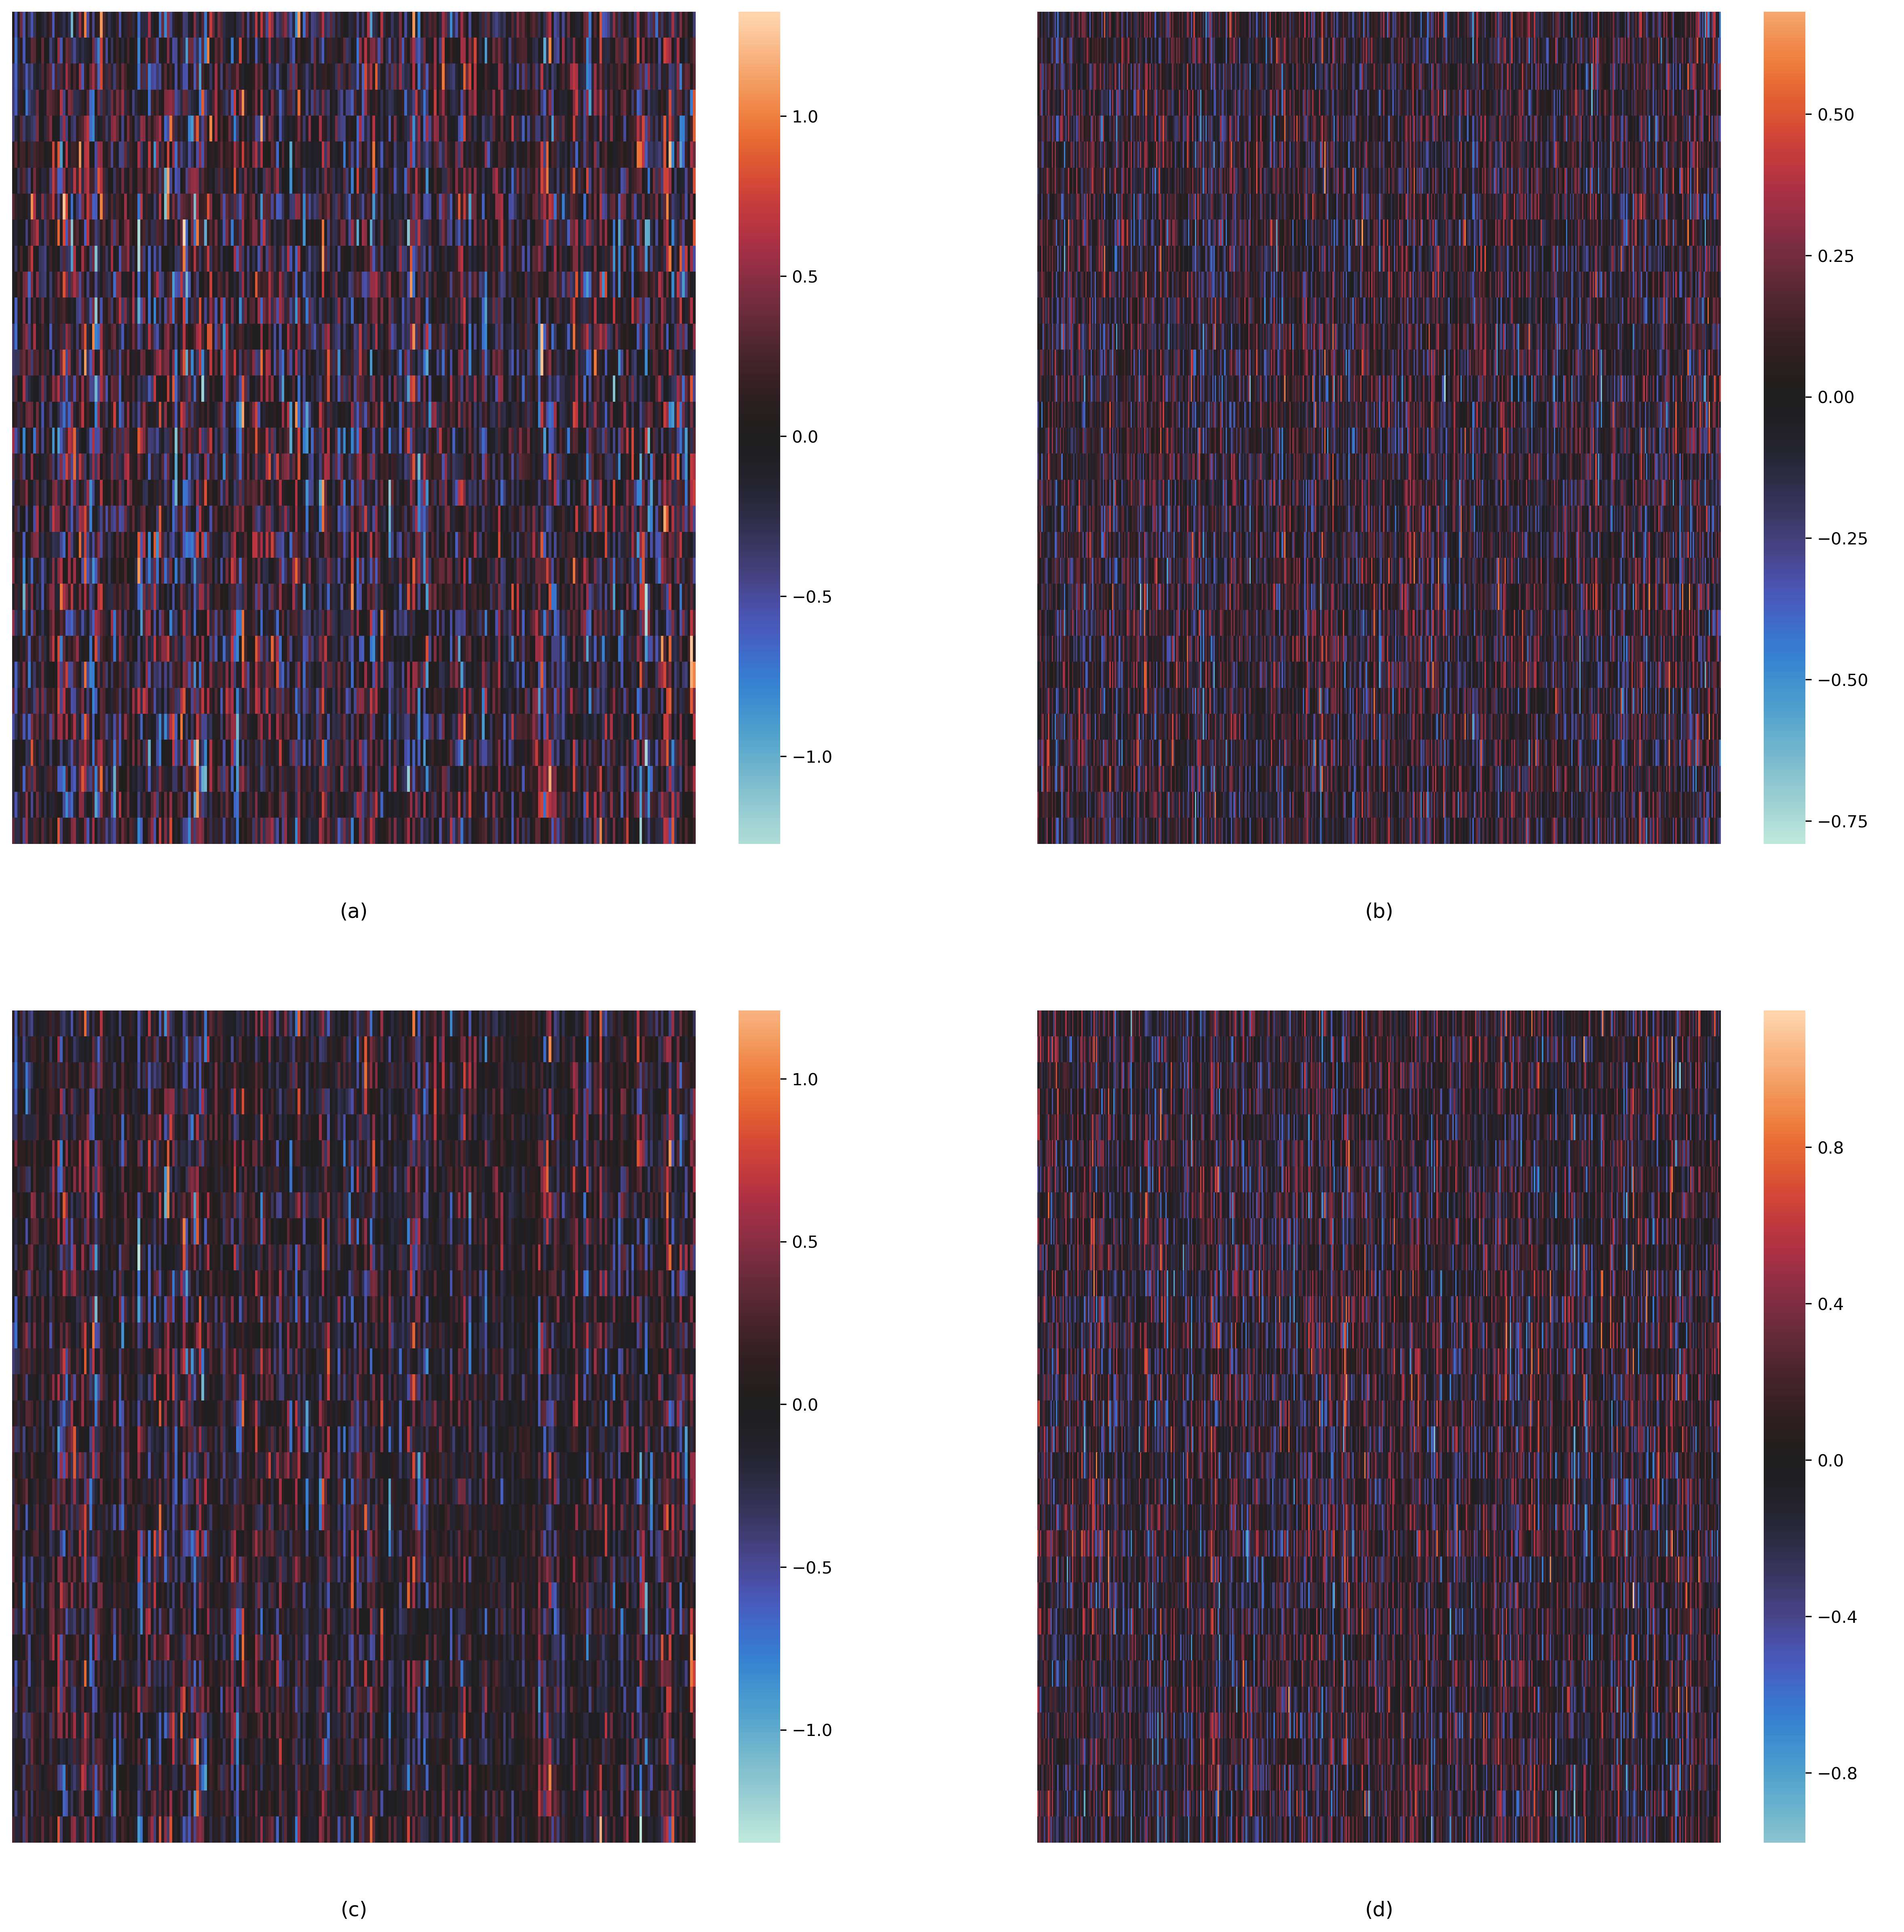
\includegraphics[width=1\textwidth]{Figure/Results/Reservoir_activity_Readout_weights_activity_.png}
 \caption{Readouts weights distribution, a, b, c and d are dynamics of reservoir-readout connections for the CIFAR-10, CIFAR-100, BSD and WS dataset.}
 \label{fig:readout_activity}
\end{figure}


In Figure~\ref{fig:readout_activity}, the elements in ${\mathbf{\Theta}}^{out}$ are small values, which implies the reservoir has sufficient capacity for the given task in each experiment, as described in Jaeger et al (2003) ~\citep{jaeger2002tutorial}. 

\subsubsection{Conclusion}


We can conclude that LS evolution problem is treated as a short-term memory problem by the CESN, because the general rule for short-term memory (i.e. fast) spectral radius should be small and for long-term memory (i.e. slow) the spectral radius should be large.  However, optimizing a reservoir with optimal performance becomes difficult due the number of parameters that drive the reservoir, and in most cases requires domain expertise.
\newpage
\subsection{CESN Global Parameter Optimization}
\label{sec:esn_global_parameter_optimization}

\subsubsection{Introduction}


In order to determine the relationship  between the memory of the reservoir and the  reservoir configuration.  We have a look at how the main global parameters parameters described in Section~\ref{sec:Global_parameters_of_the_reservoir} and how they impact the performance of the CESN in learning the evolution of the LS. For each set of the global parameters, we used the a reservoir size of 4096, spectral radius 0.9, sparsity 0.8 and leaking rate of 0.0098, when optimizing one of each parameter on the CIFAR-100 database. A total of 100 epochs are used with a decaying learning rate for each search.

\subsubsection{Results And Discussion}
% we explore leaking rate of above 1 beacuse it not a nessary condition [citation].....

In Figure~\ref{fig:esn_optimization} shows the relationship of the reservoir size, sparsity, leaking rate and spectral radius reservoir and performance in of the CESN in learning the LS.  Firstly, lets look at the reservoir size, increasing the reservoir size the recall, precision and $F_{1}Score$ increases, this is observations are expected, since the reservoir size is related to the capacity of the entire network to learn the LS, however small improvement in the performance are observed, this is likely due to the fact that optimization of larger reservoirs is difficult as pointed out by Jaeger at el, 2009~\cite{jaeger2002tutorial}. Secondly, lets look at the sparsity of the reservoir, although increasing the sparsity of the reservoir enable us to use larger reservoir sizes without incurring a high computational cost. Under the merit of this experiment increasing the sparsity of the reservoir results in a decrease in both the IoU and $F_{1}Score$, we suspect that, for more complex input images, a more powerful (and possibly more sophisticated) architecture would be required to match performance. 


\begin{figure}[H]
\centering
  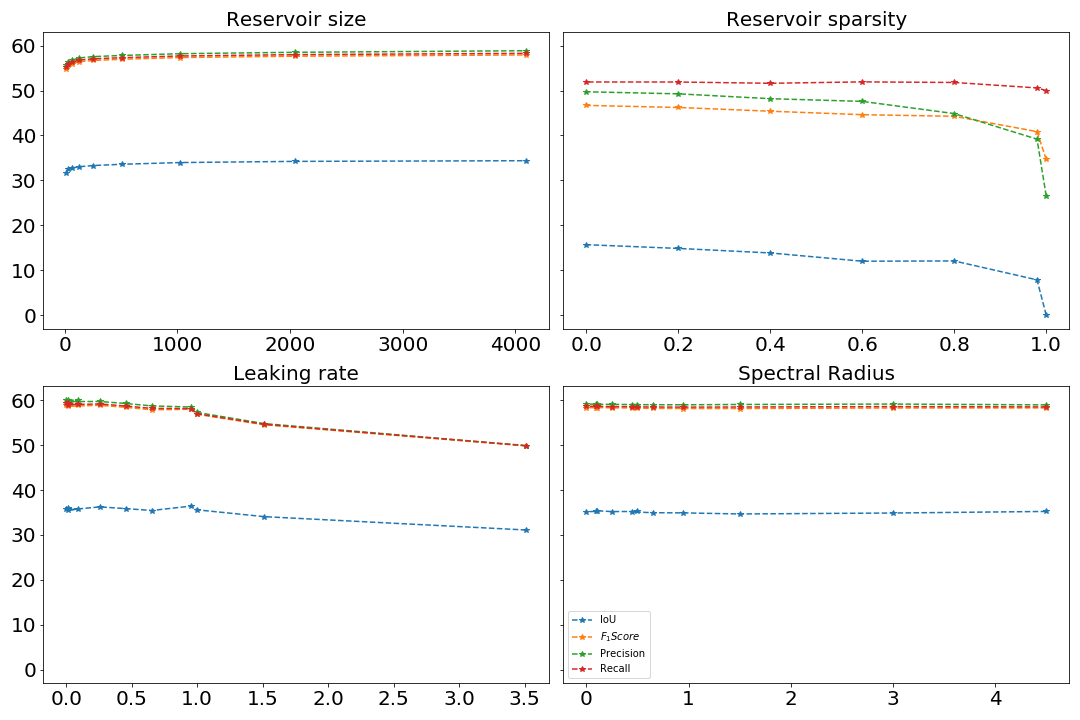
\includegraphics[width=1\textwidth]{Figure/Results/reservoir_optim.png}
 \caption{CESN optimization}
 \label{fig:esn_optimization}
\end{figure}
Thirdly, lets look at the leaking rate, increasing the leaking rate results in a increase in both the IoU and $F_{1}Score$, this suggest and validates, that the LS is a short-term memory problem, because high leaking rates are associated with problems that require less memory. This make sense, since the current segmentation only depends on the previous state of the segmentation from the LS. 
And lastly, we look at the spectral radius, increasing the spectral radius results in a slight decrease in the IoU and $F_{1}Score$, this further validates the the LS is a short-term memory problem.

In order to have non-chaotic reservoir we need to establish the echo state property is satisfied mentioned in Section~\ref{sec:echo_state_property_and_spectral_radius}. Increasing the reservoir size does improve the models performance, this is related to the capacity of the model, having a sparsity of 80\% does results in fast updated of the reservoir which are computationally cheap, however, this reduces the capacity of the reservoir, this mostly likely due to the fact that the LS is a exhibit global characteristics when determining the evolving the segmentation curve. The memory of the reservoir, or rather short-term and long-term memory, are controlled by the leaking rate and spectral radius, these parameters should be the center of attention when constructing an optimal reservoir, especially the spetral radius, since determine whether the reservoir has an echo state property.

It should be noted that noise may  have driven the optimization to a set of hyper-parameter that minimizes the error caused by the noise, which  may not be 
optimal set of parameters for prediction on the test set

\subsubsection{Conclusion}
The training episodes are relatively fast and computationally cheap compared to standard CRNN, CLSTM and CGRU since CESN does not perform back-propagation, even the with cheap computational cost, finding optimal parameters of the CESN such that the echo state property is satisfied is trivial.

\newpage


\section{Conclusion and Future Work}
\label{sec:Discussion_and_Conclusion}

In this dissertation 
This thesis proposed formulating traditional image segmentation PDE approached called levelset using deep learning-based approaches. A comparative study was conducted to determine a computationally cheap and state of the art a deep learning-based approach. The study was conducted on 2 small database the WSD and BSD and large databases CIFAR-100 and CIFAR-10.
% However, the complexity of LSTMs demands an excessive amount of computing time, making it difficult to achieve optimal performance. On the other hand, the simplicity of the ESNs can limit their generalization capabilities.

% Due to the high dimensionality of the reservoir, the numberof  parameters  of  the  prediction  model  in  (8)  would  growtoo  large,  making  the  proposed  representation  intractable.Drawbacks  in  using  large  representations  include  overfittingand  the  high  amount  of  computational  resources  to  evaluatethe  ridge  regression  solution  for  each  MTS.  In  the  contextof  RC,  applying  PCA  to  reduce  dimensionality  of  the  lastreservoir  state  has  shown  to  improve  performance  achievedon  the  inference  task  [35].  Compared  to  non-linear  methodsfor  dimensionality  reduction  such  as  kernel-PCA  or  autoen-coders  [36],  PCA  provides  competitive  generalization  capa-bilities when combined with RC models and can be computedquickly, thanks to its linear formulation 


% Although the constraints forecast hereare not conclusively better than similar results in the existing literature, in the contextof the assumptions made, the results presented here are more robust and realistic.

% Compared with the standard ESN, our ConvESN does’t addsignificant computational cost, because it still processes thesignal in linear time and the feed-forward CNN is a fixed coston top of that.Compared with other, more complex recurrent models suchas Hierarchical or Deep LSTMs, the ESN automatically pro-duces ESRs in a high-dimensional echo state space withouttraining, and has been effective in the field of (chaotic) timeseries forecasting[Jaeger and Haas, 2004]. LSTM network-s typically require extensive training via back-propagationthrough time (BPTT). For the HDM05, ConvESN-MSMCtook 157s to produce all of the 200-D action echoes from2339 sequences. Training the convnet took 23s per epoch.During testing, it runs at 780 sequences per second. Hier-archical LSTM[Duet al., 2015]reported their training timeat about real time. Our model trains about 7 times faster inequivalent circumstances, not counting the one-time genera-tion of the echo states. On the other hand, the CNN in ourframework retains the merits of weight sharing and structuralconciseness, which largely reduces the size of the parameterspace.

% In future analyses it may be interesting to consider constraints

\newpage
\bibliography{bibliography}

\end{document}
